

\documentclass[a4paper,10pt]{report} % Schriftgröße auf 10pt geändert

\usepackage{titlesec}

% FAlls ich lust hatte die seciton noch tiefer zu gehen
% \setcounter{secnumdepth}{4}
%
% \titleformat{\paragraph}
% {\normalfont\normalsize\bfseries}{\theparagraph}{1em}{}
% \titlespacing*{\paragraph}
% {0pt}{3.25ex plus 1ex minus .2ex}{1.5ex plus .2ex}

\usepackage{graphicx}
\usepackage[backend=biber]{biblatex}
\usepackage{amsmath} 
\usepackage{todonotes}
\addbibresource{citations.bib}

\usepackage{tikz}
\usetikzlibrary{automata, positioning, arrows}

% Pakete für die Verbesserungsvorschläge
\usepackage[margin=1in]{geometry} % Ränder reduziert
\usepackage{setspace} % Zeilenabstand steuern
\usepackage{enumitem} % Kompakte Listen
% \usepackage{multicol} % Mehrspaltiger Text

\usepackage{algorithmic}
\usepackage{hyperref}
\usepackage{amsmath}
\usepackage{amssymb} % oder \usepackage{amsfonts}
\usepackage{subcaption}

% \setstretch{1.15} % Zeilenabstand auf 1,15 eingestellt
% \setlist{nosep} % Kompakte Listen

\title{} % Leer lassen, da der Titel manuell gestaltet wird
\author{} % Leer lassen, da der Autor manuell gestaltet wird

\begin{document}

\begin{titlepage}
    \centering
    \vspace*{1cm}
    
    \textbf{\LARGE Optimierung eines PID-gesteuerten DC-DC-Konverters mit maschinellem Lernen}
    
    \vspace{1.5cm}
    
    \textbf{Patryk Krzyzanski}
    
    \vspace{1.5cm}
    
    Erstprüfer: Prof. Dr.-Ing. Bernhard Wicht\\
    Zweitprüfer: Dr.-Ing. Markus Olbrich
    
    \vspace{1.5cm}
    
    \textbf{Leibniz Universität Hannover}\\
    Abteilung: Institut für Mikroelektronische Systeme
    
    \vspace{1cm}
    
    \today
    
\end{titlepage}
 % Manuelle Titelseite
\begin{abstract}
In dieser Arbeit wird die Verwendung neuronaler Netze zur Optimierung und Steuerung eines PID-regulierten DC-Konverters untersucht. Das Ziel besteht darin, ein System zu entwickeln, das in der Lage ist, die altersbedingte Degradation von Schaltungskomponenten wie Kapazität und Induktivität zu überwachen und anzupassen, um die Leistung des Konverters aufrechtzuerhalten. Ein besonderer Fokus liegt auf dem Trainingsprozess und der Architektur des neuronalen Netzes. Der Trainingsprozess wird mithilfe von Methoden wie Deep Deterministic Policy Gradient (DDPG) und Bayesscher Optimierung umgesetzt. Das Training und die Schaltungssimulation werden unter Einsatz von Transientenanalyse mit SystemC durchgeführt, um eine präzise Bewertung und Auswertung der Simulationsergebnisse zu ermöglichen. Es werden Techniken zur Optimierung der Hyperparameter des neuronalen Netzes vorgestellt. Herausforderungen und Lösungsansätze im Kontext der neuronalen Netzarchitektur und des Trainings werden diskutiert. Abschließend werden die erzielten Ergebnisse und ihre Implikationen für zukünftige Forschungen präsentiert.
\end{abstract}
 % Abstract zu Beginn der Arbeit
\tableofcontents % Inhaltsverzeichnis

%\tableofcontents % Inhaltsverzeichnis

%\chapter{Einleitung}
%@START In der modernen Elektrotechnik sind DC-Konverter essentiell, um Energie effizient und präzise von einer Quelle zu einem Verbraucher zu leiten.@END [Grundlagen der Elektrotechnik]
%
%@START Mit der Zeit können jedoch Schaltungskomponenten wie Kapazitäten und Induktivitäten durch verschiedene Umwelteinflüsse degradieren, was ihre Funktionsweise beeinträchtigt.@END [Studien zur Degradation von Elektronikkomponenten]
%
%@START Hier stellt sich die Frage: Wie kann man die Leistungsfähigkeit dieser Konverter trotz solcher Alterungsprozesse aufrecht erhalten?@END [Herausforderungen bei der Wartung von Elektronikkomponenten]
%
%@START Die Antwort könnte in der Anwendung von künstlichen neuronalen Netzen liegen.@END [Einführung in künstliche neuronale Netze]
%
%
%@START In dieser Arbeit wird untersucht, wie neuronale Netze dazu genutzt werden können, um die Degradation von Schaltungskomponenten zu überwachen und die PD-Koeffizienten eines DC-Konverters entsprechend anzupassen. Dabei werden Themen wie die Architektur des Netzes, Trainingsmethoden und -umgebungen, sowie die Herausforderungen beim Training und deren Lösungsansätze behandelt.@END [Spezifische Studien zur Optimierung von DC-Konvertern mit neuronalen Netzen]

%\chapter{Einleitung} 
Die effiziente und präzise Lenkung von Energie von einer Quelle zu einem Verbraucher stellt eine zentrale Herausforderung in der modernen Elektrotechnik dar. Gleichspannungswandler (DC-DC Konverter) spielen hier eine entscheidende Rolle \cite[p.~70]{wensdesign2022}. Es existieren verschiedene Methoden zur DC-DC-Spannungsumwandlung, jede mit ihren spezifischen Vor- und Nachteilen, abhängig von unterschiedlichen Betriebsbedingungen und Spezifikationen \cite[p.~70]{wensdesign2022}.

Es wird zunehmend klar, dass bestimmte Schlüsselkomponenten, insbesondere Kapazitäten, eine Tendenz zur Degradation aufweisen. Diese Degradation ist häufig auf vielfältige Umwelteinflüsse zurückzuführen. Sie kann signifikante Auswirkungen auf die Funktionalität und Integrität der betroffenen Schaltungen haben. Daher ist es plausibel anzunehmen, dass die Lebensdauer und Effizienz von elektronischen Systemen erheblich beeinträchtigt werden könnten, wenn diese Degradationsmechanismen nicht sorgfältig betrachtet und adressiert werden.

Wissenschaftliche Untersuchungen stützen diese Beobachtungen. Jeong et al. haben in ihrem Artikel "Degradation-Sensitive Control Algorithm Based on Phase Optimization for Interleaved DC–DC Converters" spezifische Degradationsprozesse in DC-DC-Wandlern aufgezeigt. Dabei wurde insbesondere der äquivalente Serienwiderstand (ESR) von Kondensatoren als ein Hauptindikator für Degradation identifiziert \cite[p.~1]{jeong2023degradation}.

In einem ähnlichen Kontext haben Kulkarni et al. die systemischen Auswirkungen von Degradationen auf kritische Avioniksysteme hervorgehoben. Ihre Studien zeigen, dass solche Degradationen ernsthafte Konsequenzen für Navigationssysteme wie das Global Positioning System (GPS) und Inertial-Navigationssysteme haben können \cite[p.~3]{kulkarni_model-based_2023}.

Diese Erkenntnisse betonen die Notwendigkeit, die Mechanismen der Degradation elektronischer Komponenten auf Makro- und Mikroebene genau zu verstehen. Nur so können innovative Lösungen entwickelt werden, die solche Phänomene minimieren oder sogar verhindern können.

Ein vielversprechender Ansatz könnte in der Anwendung von künstlichen neuronalen Netzen (KNN) liegen. Wie Steven L. Brunton und J. Nathan Kutz in ihrem Werk "Data-Driven Science and Engineering: Machine Learning, Dynamical Systems, and Control" darlegen, bieten KNN ausgezeichnete Möglichkeiten zur Steuerung komplexer, nichtlinearer Systeme, einschließlich elektronischer Schaltungen \cite[p.~270]{brunton2019data}. Almawlawe et al. konnten in ihrer Studie zeigen, dass neuronale Netzwerk-Controller im Vergleich zu traditionellen Proportional-Integral-Derivative (PID)- und digitalen Gleitmodus-Reglern eine überlegene Leistung bei der Ausgangsspannungsverfolgung eines Buck DC/DC-Konverters bieten \cite[p.~8]{Almawlawe2023}. Miguel Morales betont in "Grokking Deep Reinforcement Learning", dass KNN einer der leistungsfähigsten Funktionsapproximatoren sind und oft andere Methoden übertreffen \cite[p.~22]{morales2020grokking}.

In dieser Arbeit wird untersucht, wie KNN dazu genutzt werden können, um die Degradation von Schaltungskomponenten zu überwachen und die PID-Koeffizienten eines DC-Konverters entsprechend anzupassen. Themen wie die Architektur des Netzes, Trainingsmethoden und -umgebungen, sowie Herausforderungen beim Training und deren Lösungsansätze werden behandelt.

\chapter{Grundlagen}




\textbf{Einleitung zum Kapitel}

Dieses Kapitel dient als umfassende Grundlage für die Erforschung der Rolle neuronaler Netze in der Optimierung und Steuerung von PID-regulierten DC-Konvertern. Im Fokus stehen sowohl die Grundlagen der DC-DC-Konvertertechnologie als auch spezielle Herausforderungen, die in diesem Kontext auftreten können, wie beispielsweise die altersbedingte Degradation von Schaltungskomponenten. Darüber hinaus bietet das Kapitel einen Überblick über moderne Optimierungsmethoden wie DDPG (Deep Deterministic Policy Gradients) und Bayessche Optimierung, die in der aktuellen Forschung Bedeutung erlangt haben.

Der Inhalt dieses Kapitels zielt darauf ab, den Leser umfassend auf die Herausforderungen, technischen Lösungen und innovativen Ansätze in diesem sich schnell entwickelnden Forschungsfeld vorzubereiten.

%1. Gleichspannungswandler (DC-DC-Konverter)


\section{Elektrotechnik}
\subsection{Buck-Konverters}

\paragraph{Hauptkomponenten und Funktionen eines DC-DC-Konverters}

Die Wandlung von Gleichspannung (DC) in eine andere Gleichspannung ist ein kritischer Aspekt in der Elektronik und Energieversorgung. Ein weit verbreitetes Schaltungsdesign, das diese Funktion ausführt, ist der Buck-Konverter. In der Literatur wird dieser als eine Standardmethode für DC-DC-Wandlung beschrieben \cite[p.~66]{wensdesign2022}.



\paragraph{MOSFET-Transistor}
Der MOSFET-Transistor agiert als elektronischer Schalter, der den Stromfluss in der Schaltung reguliert. Im Vergleich zu alternativen Schaltelementen bietet der MOSFET eine signifikante Effizienzsteigerung durch minimale Leistungsverluste. Dies wird durch Phänomene wie Trägermobilität und die damit verbundene Widerstandsfähigkeit gegenüber thermischen Ausfällen ermöglicht \cite[p.~29]{choi2013pulsewidth}.

\paragraph{Induktivität (Spule)}
Die Induktivität dient der temporären Energiespeicherung in Form eines magnetischen Feldes, das beim Stromfluss durch die Spule generiert wird. Dies ist insbesondere relevant in Anwendungen wie Solenoid-Antriebsschaltungen, wo die Induktivität als Energiespeicher und -überträger fungiert \cite[p.~54]{choi2013pulsewidth}.

\paragraph{Diode}
Die Diode ist so ausgerichtet, dass sie den Strom nur in einer Richtung passieren lässt. Dies ist insbesondere wichtig, wenn der MOSFET-Transistor deaktiviert ist. Als passive Schalter werden oftmals schnelle Erholungsdioden oder Schottky-Dioden aufgrund ihrer exzellenten Schalteigenschaften verwendet \cite[p.~29]{choi2013pulsewidth}.

\paragraph{Kondensator}
Der Kondensator dient der Glättung der Ausgangsspannung und speichert Energie für die Last. Er spielt eine wichtige Rolle in der Dynamik der Schaltung und ermöglicht eine stabilere Energieversorgung \cite[p.~54]{Kularatna2012}.
\paragraph{Regelung und Anwendungen}

In der Praxis werden Buck-Konverter oft von einer nicht-idealen Spannungsquelle gespeist und müssen daher unter variablen Eingangsspannungen und Lastströmen arbeiten \cite[p.~124,120,113]{choi2013pulsewidth}.. Daher ist eine geschlossene Regelungsschleife erforderlich, um eine konstante Ausgangsspannung sicherzustellen.

Buck-Konverter finden eine breite Anwendung in verschiedenen elektronischen Geräten und Systemen. Ihr hoher Wirkungsgrad, der in der Regel zwischen 75\% und 98\% liegt, macht sie besonders attraktiv.


\begin{figure}[htbp]
    \centering
    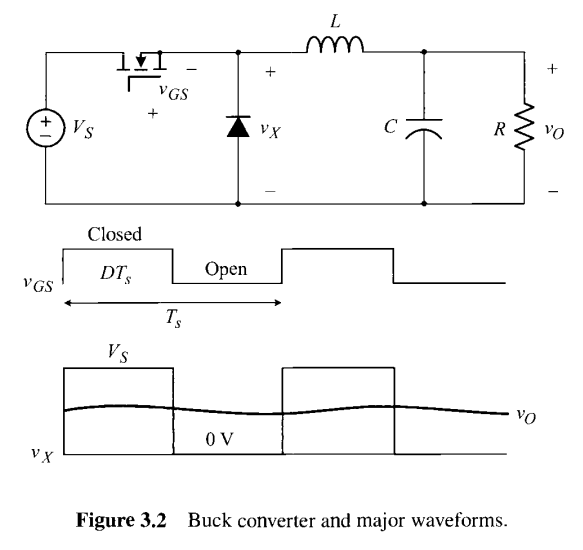
\includegraphics[width=0.4\linewidth]{2Grundlagen/111DCDC.png}
    \caption{Schematische Darstellung eines DC-DC Konverters. Quelle: \cite[Seite 88]{choi2013pulsewidth}}
    \label{fig:dcdc_converter}
\end{figure}




\subsection{Degradation von Kondensatoren und MOSFETs in DC-DC-Konvertern}

Die Zuverlässigkeit und Effizienz von DC-DC-Konvertern sind zunehmend von der Degradation ihrer Schlüsselkomponenten, insbesondere von Kondensatoren und MOSFETs, beeinträchtigt.

\paragraph{Kondensatoren}

Kondensatoren sind anfällig für verschiedene Arten von Ausfallmodi, darunter Änderungen des Verlustfaktors (tan $\delta$), der Impedanz und des Dissipationsfaktors. Diese Parameter sind entscheidend für die Beurteilung der Zuverlässigkeit eines Systems. Ebenso ist die erhöhte Äquivalente Serienresistenz (ESR) von Elektrolytkondensatoren, die elektrischen und thermischen Belastungen ausgesetzt sind, ein weiterer entscheidender Faktor für die Degradation.\cite[pp. 1]{jeong2023degradation}

\paragraph{MOSFETs}

Bei MOSFETs kann die Degradation aufgrund von thermischen Spannungen zu einem Gate-Source-Kurzschluss oder einem Drain-Source-Kurzschluss führen\. Die Degradation der Transistoren erhöht deren Leistungsverluste und beschleunigt damit den Degradationsprozess weiter.\cite[pp. 190]{wensdesign2022}



\paragraph{Kontrolle und Überwachung}

Aktuelle Forschungsbemühungen konzentrieren sich auf die Entwicklung von Kontrollalgorithmen, um die Degradation zu verzögern und die Zuverlässigkeit der Konverter zu erhöhen. Dazu gehören auch Verfahren zur Schätzung des Zustands der Degradation in Echtzeit.
\cite[p.~24, p.~310-311]{choi2013pulsewidth}

\paragraph{Integration mit neuronalen Netzen für Kondensatoren und MOSFETs}

Neuronale Netze können verwendet werden, um aktiv entgegensteuernde Maßnahmen zur Verlangsamung der Degradation von Schlüsselkomponenten wie Kondensatoren und MOSFETs in DC-DC-Konvertern einzuleiten. Durch die kontinuierliche Analyse von Betriebsparametern wie Temperatur und Spannung sind diese Netze in der Lage, den Zustand der Degradation in Echtzeit zu erfassen. Sobald kritische Zustände erkannt werden, können die neuronalen Netze automatisch die PID-Koeffizienten des Konverters anpassen, um die Degradation zu minimieren und die Zuverlässigkeit des Systems zu erhöhen.
\cite[p.~22]{morales2020grokking}

\subsection{PID-Regler}
Der PID-Regler (Proportional-Integral-Derivativ) ist eine weit verbreitete Regelungsstrategie in industriellen Steuerungssystemen und verschiedenen Arten von Anwendungen. Er ist unerlässlich für die Regelung von Prozessen wie Geschwindigkeit, Temperatur und Spannung~\cite[p.~2]{Hussein2011PIDGA}.

\paragraph{Proportionalanteil (P)}
Diese Komponente erzeugt einen Ausgangswert, der proportional zum aktuellen Fehlerwert ist. Die proportionale Reaktion kann durch Multiplikation des Fehlers mit einer Konstanten namens \( K_p \) eingestellt werden, die als Proportionalverstärkung bezeichnet wird.
\begin{equation}
P_{\text{out}} = K_p \times e(t)
\end{equation}

\paragraph{Integralanteil (I)}
Diese Komponente befasst sich mit der Akkumulation vergangener Fehler. Wenn der Fehler über einen längeren Zeitraum vorhanden war, wird er akkumuliert (Integral des Fehlers), und der Regler wird den Steuerausgang in Beziehung zu einer Konstanten \( K_i \) ändern, die als Integralverstärkung bekannt ist.
\begin{equation}
I_{\text{out}} = K_i \times \int e(t) \, dt
\end{equation}

\paragraph{Differentiantanteil (D)}
Diese Komponente liefert einen Steuerausgang, um die Änderungsrate des Fehlers zu kompensieren. Der Beitrag des Differenzierungsanteils zur gesamten Steueraktion wird als Differenzierungsverstärkung \( K_d \) bezeichnet.
\begin{equation}
D_{\text{out}} = K_d \times \frac{d}{dt} e(t)
\end{equation}
\cite[p.~1744]{russell2021ai}

\paragraph{Die PID-Regelungsgleichung}
Die PID-Regelungsgleichung kombiniert diese drei Komponenten, um den Steuerausgang zu erzeugen:
\begin{equation}
\text{Steuerausgang} = P_{\text{out}} + I_{\text{out}} + D_{\text{out}}
\end{equation}
\begin{equation}
\text{Steuerausgang} = (K_p \times e(t)) + (K_i \times \int e(t) \, dt) + (K_d \times \frac{d}{dt} e(t))
\end{equation}

\paragraph{Einstellung der Verstärkungsfaktoren}
Die Konstanten \( K_p, K_i, \) und \( K_d \) werden eingestellt, um die optimale Systemleistung zu erreichen; ein schlecht eingestellter PID-Regler kann instabil, langsam oder schwingend sein.

\paragraph{Anwendungen bei Gleichstrom-Gleichstrom-Wandlern}
Im Kontext von Gleichstrom-Gleichstrom-Wandlern können PID-Regler helfen, die Ausgangsspannung zu stabilisieren, indem sie die Ausgangsspannung kontinuierlich mit der gewünschten Spannung vergleichen und handeln, um den Fehler durch Anpassung des Tastverhältnisses des Schaltelements zu minimieren~\cite[p.~4]{Almawlawe2023}.

\paragraph{Fazit}
Der PID-Regler ist eine vielseitige und weit verbreitete Regelungsstrategie. Seine Anpassungsfähigkeit und Effizienz machen ihn ideal für eine breite Palette von Anwendungen, von industriellen Prozessen bis zu modernen Technologiesystemen. Für eine erweiterte Diskussion über verschiedene Varianten von PID-Reglern, wie zum Beispiel den Fuzzy PID-Controller, könnten Sie das Paper "Shi2020AdaptiveController" verwenden~\cite[p.~9]{Shi2020AdaptiveController}.



\subsection{Pulsweitenmodulation und ihre Darstellung}
\label{sec:PWM_Grundlagen}
Pulsweitenmodulation (PWM) ist eine Schlüsseltechnik in DC-DC-Wandlern, die zur Steuerung der Schaltkomponenten eingesetzt wird, um die Ausgangsspannung oder den Ausgangsstrom zu regulieren. Sie ermöglicht eine präzise Kontrolle, indem sie die 'Einschaltzeit' des Schalters im Vergleich zur gesamten Zykluszeit (Einschaltzeit + Ausschaltzeit) variiert.\cite{peddapelli2017pulse}

\paragraph{Tastverhältnis \(D\)}
Die Einschaltzeit ist die Zeit, der Schalter eingeschaltet ist. Das Tastverhältnis \( D \) wird mathematisch als das Verhältnis der Einschaltzeit zur gesamten Zykluszeit beschrieben:
\begin{equation}
D = \frac{\text{Einschaltzeit}}{\text{Einschaltzeit} + \text{Ausschaltzeit}}
\end{equation}

\paragraph{Proportionalanteil (P)}
Das Tastverhältnis spielt eine wichtige Rolle, da es den Mittelwert der Ausgangsspannung oder des Ausgangsstroms bestimmt. Bei der PWM wird ein Steuersignal mit einem hochfrequenten Trägersignal verglichen, um die 'Ein'- und 'Aus'-Zustände des Schalters festzulegen. Das Steuersignal stammt oft von höheren Regelkreisen wie PID-Reglern, die den Fehler zwischen Soll- und Istwert minimieren sollen.

Die Hauptmotivation für die Verwendung von PWM in Steuerungssystemen ist die Anpassung des Mittelwerts der Ausgabe an ein Referenzsignal. Zusätzlich wird versucht, harmonische Verzerrungen und Schaltverluste zu minimieren \cite{peddapelli2017pulse}.

In der Abbildung \ref{fig:PWM_converter} ist eine typische PWM-Schaltung dargestellt. Der PWM-Block und die Spannungsrückführungsschaltung im DC-DC-Wandler arbeiten zusammen, um sicherzustellen, dass die Ausgangsspannung der Referenzspannung folgt. Hierbei wird ein Steuersignal \(v_{\text{con}}\) und ein Rampensignal \(V_{\text{ramp}}\) verwendet, um die Impulsbreite des aktiven Schalters zu modulieren. Das rechte Diagramm (b) zeigt die Steuersignale und ihre Relation zueinander, wodurch das Schaltverhalten des Wandlers beeinflusst wird \cite{choi2013pulsewidth}.



\begin{figure}[htbp]
    \centering
    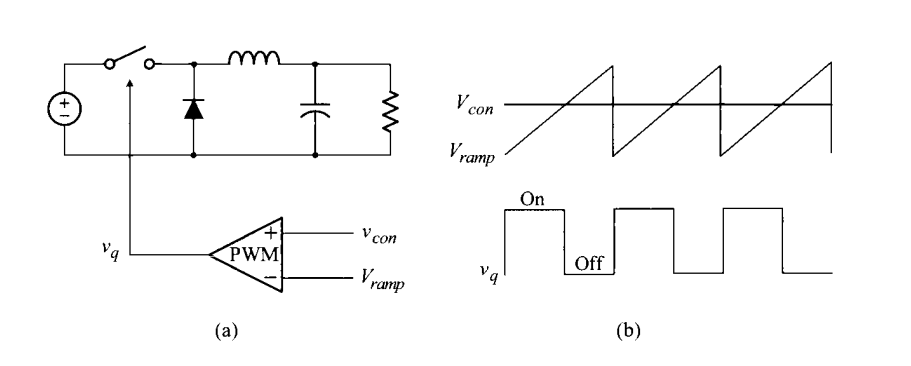
\includegraphics[width=0.8\linewidth]{2Grundlagen/141PWM.png}
    \caption{Schematische Darstellung eines PWM-Modulator. Quelle: \cite{choi2013pulsewidth}}
    \label{fig:PWM_converter}
\end{figure}


\section{Informationstechnologie}

\subsection{Einführung in Neuronale Netzwerke}
Neuronale Netzwerke bilden das rechnerische Grundgerüst für eine Vielzahl von Aufgaben in den Berei-chen maschinelles Lernen und künstliche Intelligenz. Sie sind von dem komplexen Netzwerk an Neuronen im menschlichen Gehirn inspiriert und versuchen, biologische Lernprozesse nachzuahmen \cite{aggarwal_neural_networks_2018}. In diesem Zusammenhang bieten sie ein robustes und flexibles Rahmenwerk zur Lösung komplexer Herausforderungen \cite{Goodfellow-et-al-2016}.

\subsubsection{Vorteile von Neuronalen Netzwerken}
Neuronale Netzwerke bieten mehrere entscheidende Vorteile, die ihren Einsatz in unterschiedlichen Anwendungsbereichen attraktiv machen:
\begin{itemize}
    \item \textbf{Parallelität:} Sie sind für die parallele Verarbeitung konzipiert und ermöglichen daher schnelle Berechnungen sowie Echtzeitverarbeitung.
    \item \textbf{Nichtlineare Funktionsapproximation:} Die Netzwerke sind besonders gut geeignet, nichtlineare Funktionen zu approximieren \cite{Goodfellow-et-al-2016}, was sie vielseitig einsetzbar macht.
    \item \textbf{Modellgeneralisierung:} Neuronale Netzwerke können aus einer begrenzten Datenmenge gene-ralisieren und somit präzise Vorhersagen für unbekannte Eingaben treffen.
\end{itemize}
Diese Vorteile bilden die Grundlage für ihre breite Anwendbarkeit, die im nächsten Abschnitt erläutert wird.

\subsubsection{Unterschied zwischen Biologischen und Künstlichen Neuronalen Netzwerken}
Künstliche neuronale Netzwerke bestehen aus rechnerischen Einheiten, den sogenannten Neuronen. Diese sind durch anpassbare Gewichtungen verbunden, die der Stärke synaptischer Verbindungen in biologischen Systemen ähneln. Lernen erfolgt durch die Anpassung dieser Gewichtungen, ähnlich wie sich die Stärken synaptischer Verbindungen in biologischen Systemen als Reaktion auf Reize ändern \cite{aggarwal_neural_networks_2018}.

\subsubsection{Deep Learning als Spezialisierung}
Deep Learning stellt einen spezialisierten Unterbereich des maschinellen Lernens dar, der neuronale Netzwerke mit drei oder mehr Schichten verwendet. Diese tiefen Netzwerke führen eine hierarchische Merkmalsextraktion durch, die es ihnen ermöglicht, immer komplexere Muster und Merkmale zu erkennen, während die Daten durch die Schichten fließen.

\subsubsection{Zusammenfassung und Ausblick}
Zusammenfassend bieten neuronale Netzwerke ein leistungsfähiges Rahmenwerk für eine Vielzahl von Aufgaben, von einfacher Mustererkennung bis hin zu komplexen Entscheidungsfindungsprozessen. Der Einsatz von mehrschichtigen Architekturen und nichtlinearen Aktivierungsfunktionen erweitert die Fähig-keiten traditioneller maschineller Lernalgorithmen \cite{aggarwal_neural_networks_2018}.

Mit dieser Grundlage werden die folgenden Abschnitte einen vertieften Einblick in die mathematischen Aspekte von neuronalen Netzwerken bieten. Insbesondere werden wir uns darauf konzentrieren, wie neuronale Netzwerke bei der Optimierung und Steuerung von PID-regulierten DC-Konvertern Anwendung finden. Dabei liegt der Fokus auf der Berücksichtigung von Alterungsprozessen und Abnutzung von Schaltungselementen wie Kapazitäten und Induktivitäten und wie diese Einflüsse mathematisch modelliert und optimiert werden können.

\subsection{Vorwärtspropagation in Neuronalen Netzwerken}
\subsubsection{Schicht-für-Schicht-Propagation}
Beginnend mit der Eingabeschicht \( A^{[0]} \), die im Wesentlichen die Eingabedaten \( X \) sind, berechnet jede nachfolgende Schicht \( Z^{[l]} \) und \( A^{[l]} \) entsprechend den oben genannten Gleichungen. Dies bildet das Kernstück der Vorwärtspropagation.

\subsubsection{Dimensionalität und Netzwerkarchitektur}
Die Anzahl der Neuronen in jeder Schicht und die Art der verwendeten Aktivierungsfunktion können die Leistung des Netzwerks erheblich beeinflussen. Es ist wichtig, die Dimensionalität jeder Schicht während der Entwurfsphase zu berücksichtigen, um ein effektives Lernen sicherzustellen.

Die Vorwärtspropagation ist ein wesentlicher Prozess in neuronalen Netzwerken, der die Übertragung von Eingabedaten durch die Netzwerkarchitektur ermöglicht, um die Ausgabe zu erzeugen \cite[p.~1421]{russell2021ai}. Sie ist eine Abfolge von mathematischen Operationen, die Gewichtungen, Biases und Aktivierungsfunktionen involvieren \cite[p.~73]{Chollet2021}.

\subsubsection{Gewichtsmatrix \( W^{[l]} \) und Bias-Vektor \( b^{[l]} \)}
Die Gewichtsmatrix für die Schicht \( l \) wird als \( W^{[l]} \) bezeichnet, und \( b^{[l]} \) ist der Bias-Vektor für dieselbe Schicht \cite[p.~46]{heaton_2012}. Diese Parameter werden während des Backpropagation-Prozesses trainiert, um den Fehler zwischen der vorhergesagten und der tatsächlichen Ausgabe zu minimieren \cite[p.~41]{aggarwal_neural_networks_2018}.

\begin{equation}
Z^{[l]} = W^{[l]} A^{[l-1]} + b^{[l]}
\end{equation}

\subsubsection{Aktivierungsfunktionen}
Eine Aktivierungsfunktion, normalerweise durch \( \sigma \) bezeichnet, transformiert die gewichtete Summe \( Z^{[l]} \) in die aktivierte Ausgabe \( A^{[l]} \) \cite[p.~1421]{russell2021ai}.

\begin{equation}
A^{[l]} = \sigma(Z^{[l]})
\end{equation}

\begin{equation}
A^{[l]} = \sigma \left( 
\begin{pmatrix}
w_{1,1}^{[l-1,l]} & w_{1,2}^{[l-1,l]} & \cdots & w_{1,m}^{[l-1,l]} \\
w_{2,1}^{[l-1,l]} & w_{2,2}^{[l-1,l]} & \cdots & w_{2,m}^{[l-1,l]} \\
\vdots & \vdots & \ddots & \vdots \\
w_{n,1}^{[l-1,l]} & w_{n,2}^{[l-1,l]} & \cdots & w_{n,m}^{[l-1,l]}
\end{pmatrix}
\begin{pmatrix}
A_1^{[l-1]} \\
A_2^{[l-1]} \\
\vdots \\
A_m^{[l-1]}
\end{pmatrix}
+
\begin{pmatrix}
b_1^{[l]} \\
b_2^{[l]} \\
\vdots \\
b_n^{[l]}
\end{pmatrix}
\right)
\end{equation}

\subsubsection{Schicht-für-Schicht-Propagation}
Beginnend mit der Eingabeschicht \( A^{[0]} \), die im Wesentlichen die Eingabedaten \( X \) sind, berechnet jede nachfolgende Schicht \( Z^{[l]} \) und \( A^{[l]} \) entsprechend den oben genannten Gleichungen \cite[p.~1421]{russell2021ai}.

\subsubsection{Dimensionalität und Netzwerkarchitektur}
Die Anzahl der Neuronen in jeder Schicht und die Art der verwendeten Aktivierungsfunktion können die Leistung des Netzwerks erheblich beeinflussen \cite[p.~1408]{russell2021ai}. Es ist wichtig, die Dimensionalität jeder Schicht während der Entwurfsphase zu berücksichtigen, um ein effektives Lernen sicherzustellen \cite[p.~73]{Chollet2021}.


\subsection{Gradientenberechnung}

Sie haben eine Kostenfunktion \( C_0 \) definiert als:
\begin{equation}
C_0 = \sum_{j=0}^{n_{L-1}} (a_j^{[L]} - y_j)^2
\end{equation}

Um die Kostenfunktion zu minimieren, müssen Sie den Gradienten in Bezug auf alle Gewichtungen und Bias berechnen. Mit Hilfe der Kettenregel können Sie die partielle Ableitung der Kostenfunktion in Bezug auf jedes Gewicht wie folgt ausdrücken:

\begin{equation}
\frac{\partial C_0}{\partial w_{jk}^{[L]}} = \frac{\partial w_{jk}^{[L]}}{\partial z_j^{[L]}} \frac{\partial z_j^{[L]}}{\partial a_j^{[L]}} \frac{\partial a_j^{[L]}}{\partial C_0}
\end{equation}

Wenn Sie den Nabla-Operator verwenden, um den Gradienten der Kostenfunktion in Bezug auf alle Gewichtungen in der Matrixform darzustellen, erhalten Sie:

\begin{equation}
\nabla_{W^{[L]}} C_0 = \begin{pmatrix}
\frac{\partial C_0}{\partial w_{11}^{[L]}} & \frac{\partial C_0}{\partial w_{12}^{[L]}} & \cdots & \frac{\partial C_0}{\partial w_{1m}^{[L]}} \\
\frac{\partial C_0}{\partial w_{21}^{[L]}} & \frac{\partial C_0}{\partial w_{22}^{[L]}} & \cdots & \frac{\partial C_0}{\partial w_{2m}^{[L]}} \\
\vdots & \vdots & \ddots & \vdots \\
\frac{\partial C_0}{\partial w_{n1}^{[L]}} & \frac{\partial C_0}{\partial w_{n2}^{[L]}} & \cdots & \frac{\partial C_0}{\partial w_{nm}^{[L]}}
\end{pmatrix}
\end{equation}

Dabei ist \( \nabla_{W^{[L]}} C_0 \) die Matrix der partiellen Ableitungen der Kostenfunktion \( C_0 \) in Bezug auf jede Gewichtung in \( W^{[L]} \).



\subsection{Rückpropagation in Neuronalen Netzwerken}

Für die Rückpropagation definieren wir den Fehler in der Ausgabeschicht durch:
\[
\frac{\partial C_0}{\partial a_j^{[L]}} = 2 \left( a_j^{[L]} - y_j \right)
\]
wobei \( a_j^{[L]} \) die Aktivierung der \( j \)-ten Einheit in der Ausgabeschicht und \( y_j \) der tatsächliche Wert für diese Einheit ist.

\paragraph{Fehler Rückpropagieren}

Der nächste Schritt besteht darin, den Fehler durch das Netzwerk zurückzupropagieren. Um den Beitrag jeder Gewichtung und jedes Bias zur Gesamtkostenfunktion zu ermitteln, berechnen wir die Ableitung der Aktivierungsfunktion \( a_j^{[L]} \) in Bezug auf die lineare Kombination \( z_j^{[L]} \):
\[
\frac{\partial z_j^{[L]}}{\partial a_j^{[L]}} = \sigma' \left( z_j^{[L]} \right)
\]
wobei \( \sigma' \left( z_j^{[L]} \right) \) die Ableitung der Aktivierungsfunktion ist.

Um die Ableitung der linearen Kombination \( z_j^{[L]} \) in Bezug auf die Gewichtung \( w_{jk}^{[L]} \) zu berechnen, verwenden wir:
\[
\frac{\partial z_j^{[L]}}{\partial w_{jk}^{[L]}} = a_k^{[L-1]}
\]

\paragraph{Kettenregel Anwenden}

Jetzt kombinieren wir alle diese Teile mit der Kettenregel:
\[
\frac{\partial C_0}{\partial w_{jk}^{[L]}} = 2 \left( a_j^{[L]} - y_j \right) \cdot \sigma' \left( z_j^{[L]} \right) \cdot a_k^{[L-1]}
\]

\paragraph{Gradienten der Kostenfunktion}

Schließlich, um den Gradienten der Kostenfunktion \( C_0 \) in Bezug auf alle Gewichtungen darzustellen, verwenden wir:
\[
\nabla W^{[L]} C_0 = \left( 2 \left( a^{[L]} - y \right) \odot \sigma' \left( Z^{[L]} \right) \right) A^{[L-1]T}
\]

Mit diesen Gradienten können Sie die Gewichtungen und Biasse im neuronalen Netzwerk aktualisieren, indem Sie einen Optimierungsansatz wie den Gradientenabstieg verwenden.

\subsection{Backpropagation im Training neuronaler Netze}

\subsubsection{Mathematische Grundlagen}

Die Gradientenmatrix für die Gewichtungen in Bezug auf die Kostenfunktion \( C_0 \) unter Verwendung des Nabla-Operators kann in der Matrixform dargestellt werden:

Dabei setzt sich jede Komponente der Matrix wie folgt zusammen:

\[
\frac{\partial C_0}{\partial w_{ij}^{[L]}} = 2(a_i^{[L]} - y_i) \cdot \sigma' (z_i^{[L]}) \cdot a_j^{[L-1]}
\]

So erhalten wir die gesamte Matrix der partiellen Ableitungen:

\[
\nabla_{W^{[L]}} C_0 = 
\begin{pmatrix}
2(a_1^{[L]} - y_1) \cdot \sigma' (z_1^{[L]}) \cdot a_1^{[L-1]} & \cdots & 2(a_1^{[L]} - y_1) \cdot \sigma' (z_1^{[L]}) \cdot a_m^{[L-1]} \\
2(a_2^{[L]} - y_2) \cdot \sigma' (z_2^{[L]}) \cdot a_1^{[L-1]} & \cdots & 2(a_2^{[L]} - y_2) \cdot \sigma' (z_2^{[L]}) \cdot a_m^{[L-1]} \\
\vdots & \ddots & \vdots \\
2(a_n^{[L]} - y_n) \cdot \sigma' (z_n^{[L]}) \cdot a_1^{[L-1]} & \cdots & 2(a_n^{[L]} - y_n) \cdot \sigma' (z_n^{[L]}) \cdot a_m^{[L-1]}
\end{pmatrix}
\]

Die Größe dieser Matrix ist \( n \times m \), wobei \( n \) die Anzahl der Neuronen in Schicht \( L \) und \( m \) die Anzahl der Neuronen in Schicht \( L-1 \) ist.

Jeder Eintrag in dieser Matrix gibt die Änderungsrate der Kostenfunktion \( C_0 \) in Bezug auf das entsprechende Gewicht an. Mit dieser Matrix können Sie die Gewichtungen in Schicht \( L \) aktualisieren, um die Kostenfunktion zu minimieren.






%Informationstechnologie
  %Einleitung und Bedeutung der IT

%Grundlagen Neuronaler Netze
  %Einleitung und Historie
  %Nichtlineare Approximation
  %Architekturen neuronaler Netze (Feedforward, CNN, RNN)
  %Einführungsbeispiel: Funktionsapproximation
  %Fehlerberechnung und Kostenfunktion

%Optimierungsverfahren
  %Gradient Descent
  %Backpropagation
  %Advanced Optimizers (Adam, RMSprop)

%Hyperparameter und Regularisierung
  %Learning Rate
  %Batch Size
  %Overfitting und Regularisierung
  %Datenvorbereitung und -transformation
  %Normalization (Batch, Layer)
  
%Aktivierungsfunktionen
  %Sigmoid, ReLU, Tanh etc.

%Evaluationsmetriken
  %Klassifikation: Genauigkeit, F1-Score etc.
  %Reinforcement Learning: Reward-Metriken

%Reinforcement Learning
  %Grundlagen und Prinzipien
  %Markov-Entscheidungsprozesse (MDPs)
  %Belohnungssystem
  %Exploration vs Exploitation
  %Policy vs. Value-based Methods

%Regularisierung in RL
  %Entropie-Regularisierung etc.

%Fortgeschrittene Themen in Deep Learning
  %Deep Q-Learning
  %Actor-Critic-Methoden
  %DDPG (Deep Deterministic Policy Gradients)


%^
%^#### 3. Technische Umsetzung / Implementierung und Software-Architektur
%^- Programmiersprachen und Bibliotheken
%^  - C++
%^  - TensorFlow
%^  - Python
%^  - SystemC
%^- Schnittstellen-Design
%^  - API-Entwicklung
%^  - Modulare Architektur
%^- SystemC in der Schaltungssimulation
%^  - Grundlagen
%^  - Transientenanalyse
%^  - Vorteile und Herausforderungen
%^- Implementierungsdetails
%^  - Code-Architektur
%^  - Optimierung für Performanz
%^
%^---
%^
%^Die Bezeichnung "Technische Umsetzung" oder "Implementierung und Software-Architektur" für den dritten Teil würde in diesem Kontext sehr gut passen, da es sowohl den Programmcode als auch die spezifischen Software-Tools abdeckt, die für die Umsetzung der in den Grundlagen vorgestellten Konzepte erforderlich sind. So schaffen Sie eine klare Abgrenzung zu den vorherigen Teilen, die sich mehr mit den theoretischen Grundlagen befassen.













%Die Informationstechnologie (IT) hat eine tiefgreifende und weitreichende Wirkung auf fast jeden Aspekt der modernen Gesellschaft, einschließlich Wissenschaft, Industrie, Bildung und Alltagsleben. Die historische Entwicklung der IT ist ein faszinierendes Thema, das sich von den Anfängen der mechanischen Rechenmaschinen bis zu den heutigen Supercomputern und Cloud-Infrastrukturen erstreckt.
%
%### Frühe Anfänge
%Die Wurzeln der IT gehen auf mechanische Rechenmaschinen wie die Pascaline von Blaise Pascal und die Leibnizsche Rechenmaschine zurück. Diese Vorläufer der modernen Computer waren jedoch in ihren Fähigkeiten sehr eingeschränkt.
%
%### Das Zeitalter der Elektronischen Computer
%Mit dem Aufkommen der ersten elektronischen Computer in den 1940ern, wie dem ENIAC und dem UNIVAC, begann die moderne Ära der Informationstechnologie. Diese Maschinen verwendeten Vakuumröhren und waren oft raumgroß, aber sie legten den Grundstein für die Entwicklung kleinerer, leistungsfähigerer und effizienterer Systeme.
%
%### Miniaturisierung und Massenmarkt
%Der Übergang von Vakuumröhren zu Transistoren und später zu integrierten Schaltkreisen führte zur Miniaturisierung von Computern. Der Personal Computer (PC) revolutionierte in den 1980er Jahren die Zugänglichkeit von Computern für die breite Öffentlichkeit. 
%
%### Internet und Globalisierung
%Das Aufkommen des Internets in den 1990ern veränderte die Art und Weise, wie wir kommunizieren, Geschäfte tätigen und Informationen teilen. Es führte zu einer noch nie dagewesenen Globalisierung und Vernetzung.
%
%### Einfluss auf die Wissenschaft
%In der Wissenschaft hat die IT die Forschungsmethoden und -möglichkeiten erheblich erweitert. Supercomputer ermöglichen komplexe Simulationen in Bereichen wie Klimaforschung, Genomik und Materialwissenschaft. Datenanalyse-Tools haben das Handling von großen Datensätzen erleichtert, und künstliche Intelligenz hat Bereiche wie maschinelles Lernen und automatische Entscheidungsfindung vorangetrieben.
%
%### Einfluss auf die Industrie
%In der Industrie hat die IT Produktionsprozesse optimiert, die Lieferkette effizienter gemacht und den globalen Handel erleichtert. Automatisierung, Prozesskontrolle und Qualitätssicherung sind nur einige der Bereiche, die durch die IT revolutioniert wurden.
%
%Die fortschreitende Entwicklung in der Informationstechnologie zeigt keine Anzeichen einer Verlangsamung, mit fortlaufenden Innovationen in Bereichen wie Künstlicher Intelligenz, Internet der Dinge (IoT) und Quantencomputing. Diese Technologien versprechen, die Art und Weise, wie wir leben und arbeiten, weiter zu transformieren.

\chapter{Realisierung}




\section{Motivation und Zielsetzung}

Das zentrale Anliegen dieser Arbeit ist die Entwicklung eines effizienten Agenten, basierend auf den Prinzipien des Reinforcement Learning, der in der Lage ist, auf Degenerationsprozesse in elektronischen Schaltungen zu reagieren. Dieser Agent soll durch ein neuronales Netzwerk realisiert werden und in der Lage sein, optimale PID-Reglereinstellungen für sich verändernde Degenerationszustände innerhalb einer Schaltung zu bestimmen. Ein DC-DC-Konverter dient als Ausgangsmodell, um den Agenten zu trainieren und die grundlegenden Prinzipien zu veranschaulichen, mit dem Ziel, eine generalisierbare Lösung zu entwickeln, die auf unterschiedliche Schaltungskontexte anwendbar ist.

\section{Herausforderungen und Ziele}

Die Entwicklung eines leistungsfähigen Reinforcement-Learning-Systems stellt mehrere Herausforderungen dar, die in diesem Experiment adressiert werden müssen:

\begin{enumerate}
    \item \textbf{Agentenwahl und -konfiguration:} Die Auswahl und Konfiguration des Agenten, insbesondere die Architektur des neuronalen Netzes, sind entscheidend, um effektives Lernen zu gewährleisten. Der Agent muss in der Lage sein, die komplexen Zusammenhänge zwischen den Zuständen der Schaltung und den entsprechenden Aktionen zu erfassen.
    
    \item \textbf{Aufbau einer effizienten Simulation:} Eine Simulation, die schnell genug ist, um zeitnahe Trainingsdurchläufe zu ermöglichen, ist für die Konvergenz des Modells von entscheidender Bedeutung. Die Simulationsumgebung muss akkurate Rückmeldungen in einer Zeitspanne liefern, die praktikables und iteratives Training zulässt.
    
    \item \textbf{Bestimmung der Reward-Funktion:} Die Definition einer angemessenen Reward-Funktion ist essentiell, um das Agentenverhalten in Richtung der gewünschten Zielvorgaben zu lenken. Die Reward-Funktion muss so gestaltet sein, dass sie das System zuverlässig zum gewünschten Leistungsziel führt.
    
    \item \textbf{Validierung des trainierten Netzwerks:} Neuronale Netzwerke können oft auch unter suboptimalen Einstellungen zufriedenstellende Ergebnisse liefern. Die eigentliche Herausforderung besteht darin, das Modell so zu trainieren, dass es die Gegebenheiten und Dynamiken der Simulationsumgebung nicht nur nachahmt, sondern auch versteht und die Leistungsfähigkeit der Schaltung präzise verbessert.
\end{enumerate}

Die Überwindung dieser Herausforderungen erfordert einen methodischen Ansatz, der die Interaktion zwischen den Komponenten des Systems detailliert analysiert und optimiert. 

\section{Wahl der Architektur und verwendete Technologien}
\label{sec:integration_rl_simulation}

\begin{figure}[htbp]
\centering
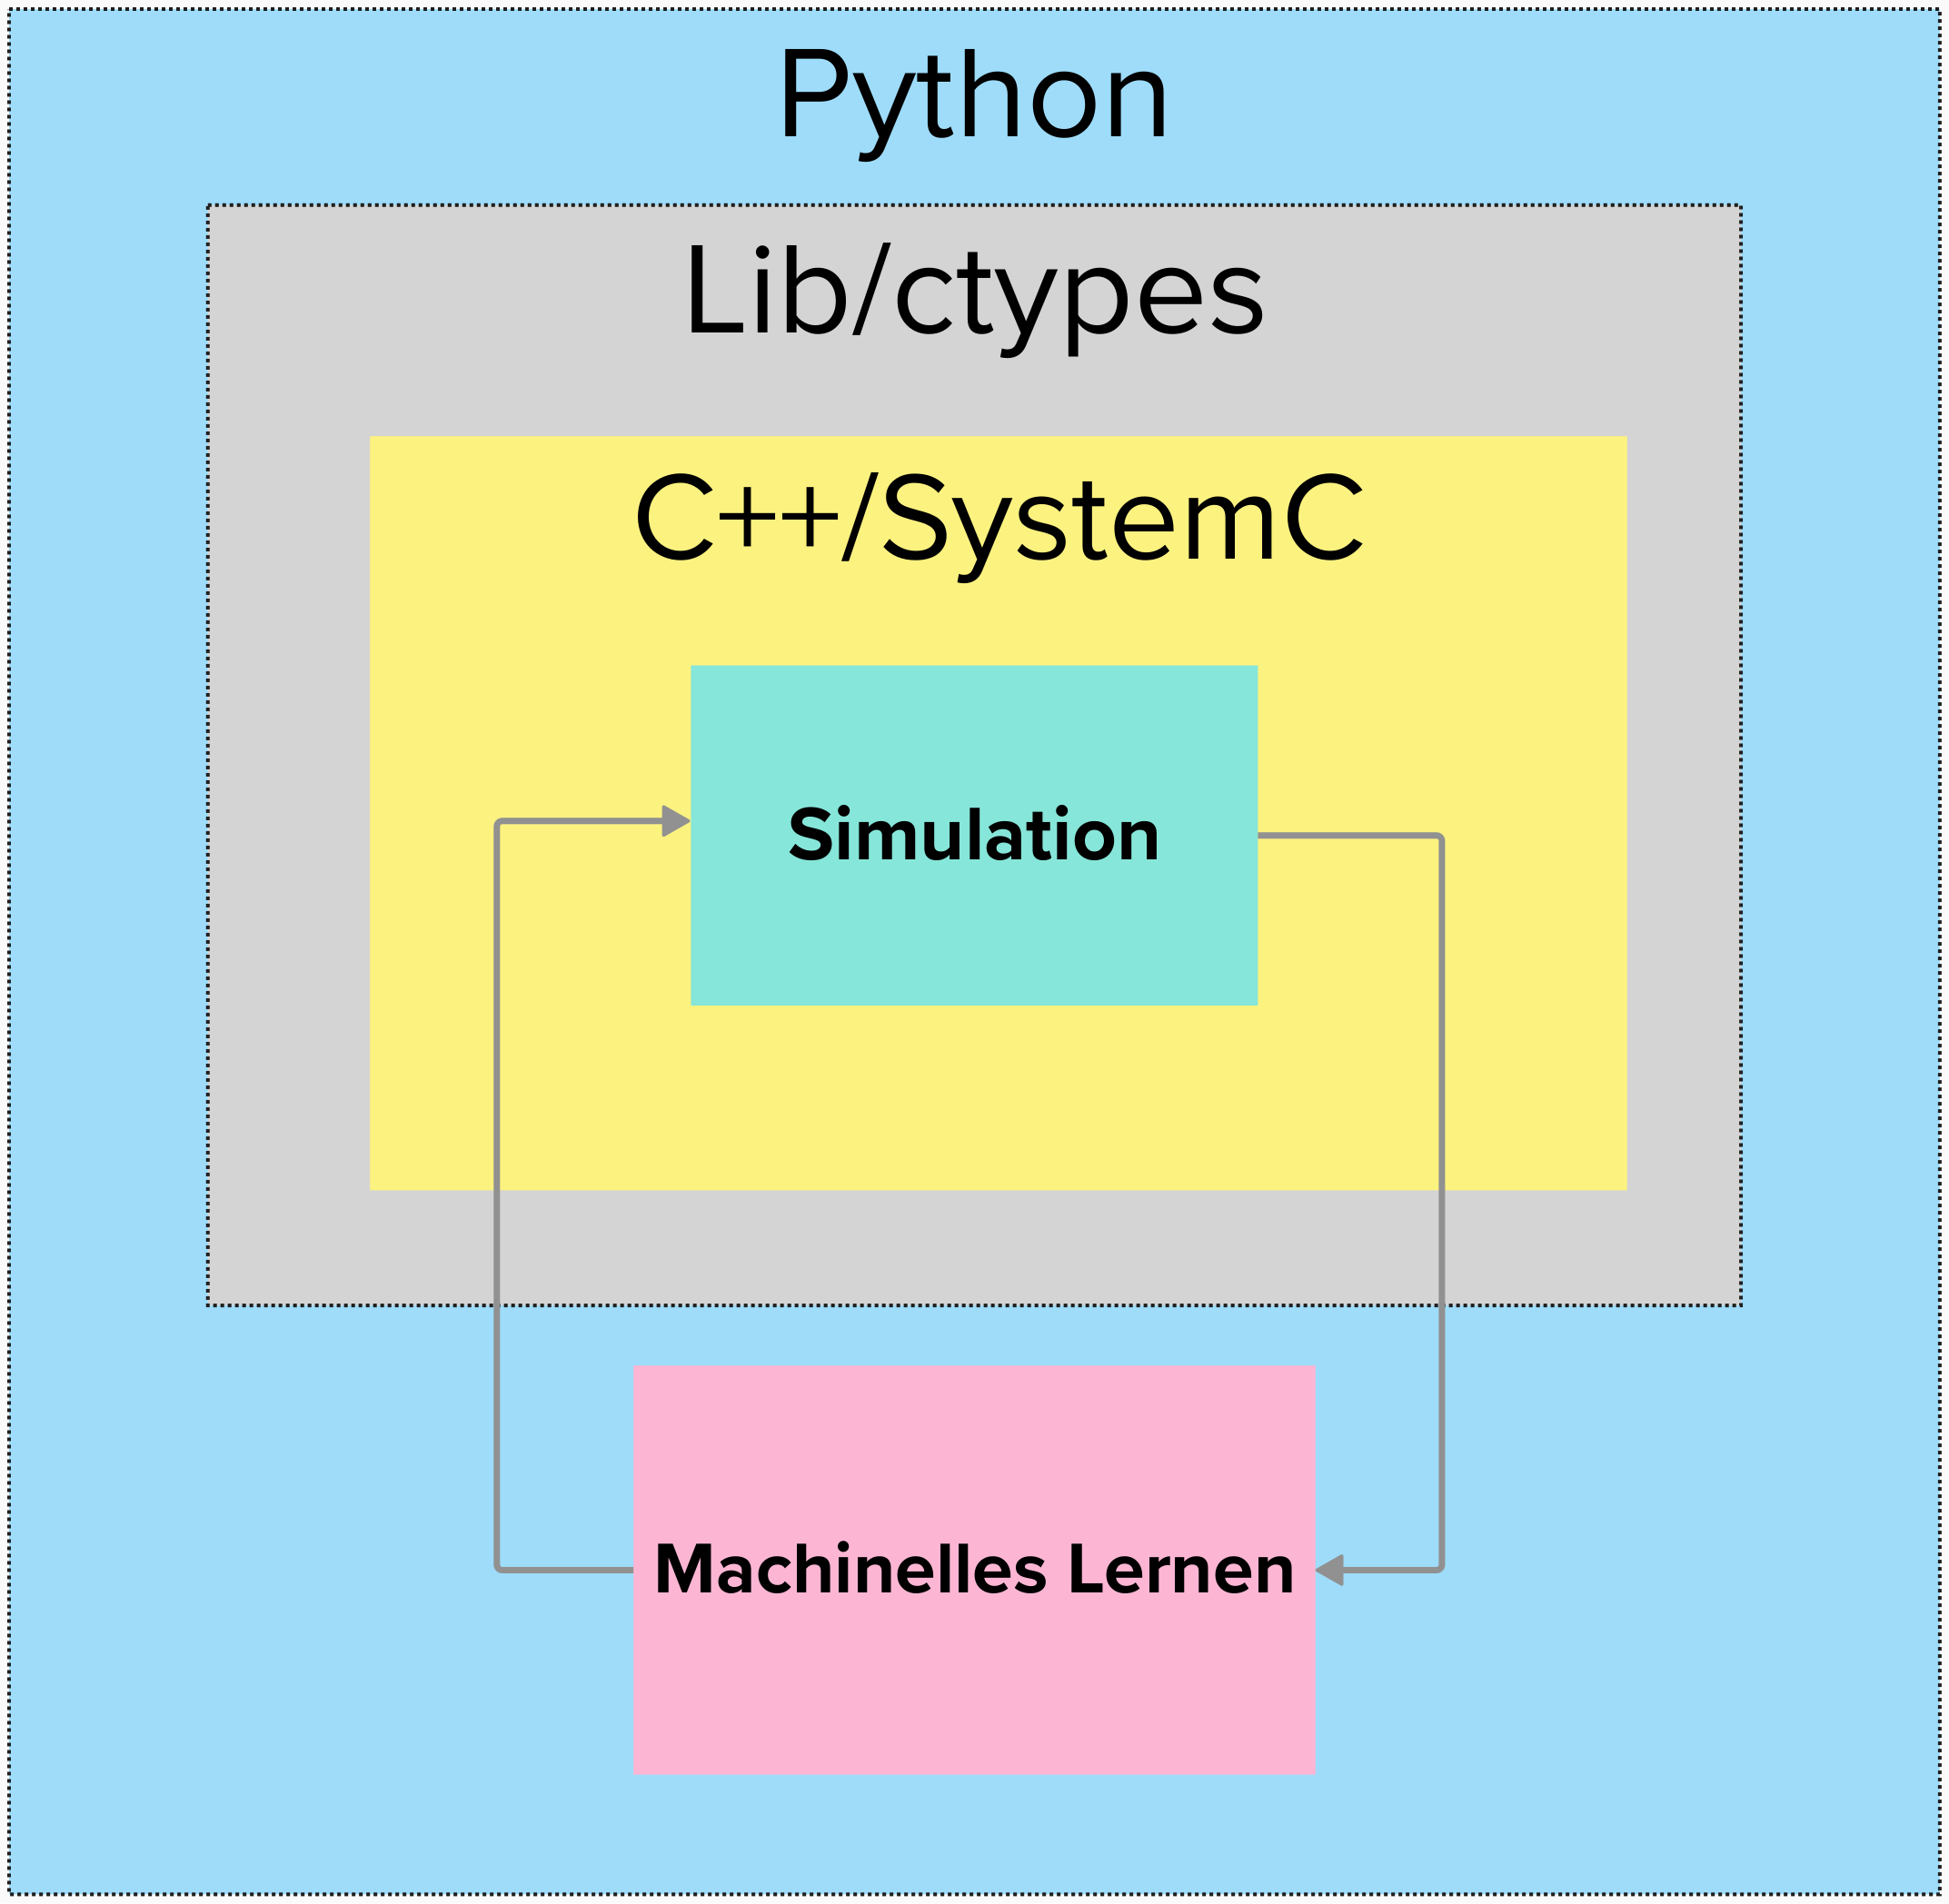
\includegraphics[width=0.4\linewidth]{3Experiment/1SystemC_Wahl_Architectur.png}
\caption{Die Architektur des integrierten Systems, das die Schaltungssimulation und das maschinelle Lernen verbindet.}
\label{fig:integrated_system_architecture}
\end{figure}

Für das Experiment wurden spezifische Technologien und Architekturen ausgewählt, die optimal auf die Anforderungen der Problemstellung abgestimmt sind. Die Entscheidung fiel auf eine Kombination aus Python für die Implementierung des Reinforcement Learning-Teils und SystemC mit C++ für die Simulation der elektronischen Schaltung.

\subsection{Reinforcement Learning mit Python}
Der Reinforcement Learning-Teil des Experiments wurde in Python entwickelt, unter Verwendung von modernen Frameworks wie TensorFlow 2 und Keras. Diese Bibliotheken erleichtern den Entwurf und das Training von neuronalen Netzwerken durch ihre hohe Abstraktion und Benutzerfreundlichkeit. Zusätzlich wurde CUDA verwendet, um das Training der Modelle auf Grafikkarten zu beschleunigen und somit die Konvergenzzeit signifikant zu reduzieren.

\subsection{SystemC und C++ für die Schaltungssimulation}
Der Teil des Experiments, der sich auf die elektronische Schaltung bezieht, wurde in SystemC implementiert, einem C++ basierten Modellierungsframework, das sich durch seine Fähigkeit zur schnellen und präzisen Simulation von Hardwarekomponenten auszeichnet. SystemC bietet eine hohe Modularität und Eignung für die Entwicklung komplexer Schaltungssysteme und ermöglicht eine detaillierte Analyse der Schaltungsverhalten unter verschiedenen Bedingungen.

\paragraph{Integration von Python und SystemC}
Die Integration der in Python entwickelten Reinforcement Learning-Komponente mit der in SystemC implementierten Schaltungssimulation stellt eine besondere technische Herausforderung dar. Diese wurde durch den Einsatz spezialisierter Schnittstellen und Protokolle gemeistert, welche die beiden unterschiedlichen Umgebungen miteinander kompatibel machen und einen reibungslosen Datenaustausch gewährleisten.

\paragraph{Lib/ctypes als Brücke}
Lib/ctypes ist eine Bibliothek in Python, die es ermöglicht, C-Funktionen innerhalb der Python-Umgebung aufzurufen. Dies erlaubt eine effiziente Integration der C++-basierten Schaltungssimulation in das Python-basierte Lernmodell, ohne dass die Leistung darunter leidet.

\paragraph{Modulare und erweiterbare Softwareentwicklung}
Die gesamte Entwicklung folgte den Prinzipien der Kapselung, objektorientierten Programmierung und Interface-gesteuerten Design, was die spätere Anpassung und Erweiterung auf andere Schaltungsmodelle ermöglicht. Dieser modulare Ansatz trägt dazu bei, dass die entwickelten Lösungen auch in anderen Kontexten und für verschiedene Schaltungstypen anwendbar sind.



Für das Kernstück des Experiments, die Wahl der geeigneten Reinforcement Learning-Architektur, fiel die Entscheidung auf den Deep Deterministic Policy Gradient (DDPG). Dieser Ansatz bietet mehrere Vorteile, die ihn für das vorliegende Experiment besonders qualifizieren. Bei der Wahl der Architektur für dieses Experiment wurden drei Hauptgründe berücksichtigt:

\begin{itemize}
    \item Behandlung kontinuierlicher Aktionsräume: Die gewählte Architektur kann effektiv mit kontinuierlichen Aktionsräumen umgehen, was für analoge Anwendungen und reale Einsatzgebiete entscheidend ist.
    \item Schnelle Konvergenz: Der Deep Deterministic Policy Gradient (DDPG) zeichnet sich durch seine schnelle Konvergenz aus. Da die Simulationen im Experiment zeitaufwendig sind, ist eine zügige Konvergenz wichtig für die Effizienz des Trainingsprozesses.
    \item Modularität der Architektur: Die aus Äktor (Actor) und Kritiker (Critic) bestehende Architektur ermöglicht eine Variation von Gewichten und Schichten in getrennten Netzwerkteilen, was besonders bei der Übertragung des Modells auf physische Implementierungen wie einen Mikrochip von Vorteil ist.
\end{itemize}

Die Architektur wurde also aufgrund ihrer Eignung für kontinuierliche Aktionsräume, ihrer schnellen Konvergenz und ihrer Modularität ausgewählt, um den Anforderungen des Experiments gerecht zu werden.

\section{Überblick über den Aufbau und Datenfluss}

\begin{figure}[htbp]
\centering
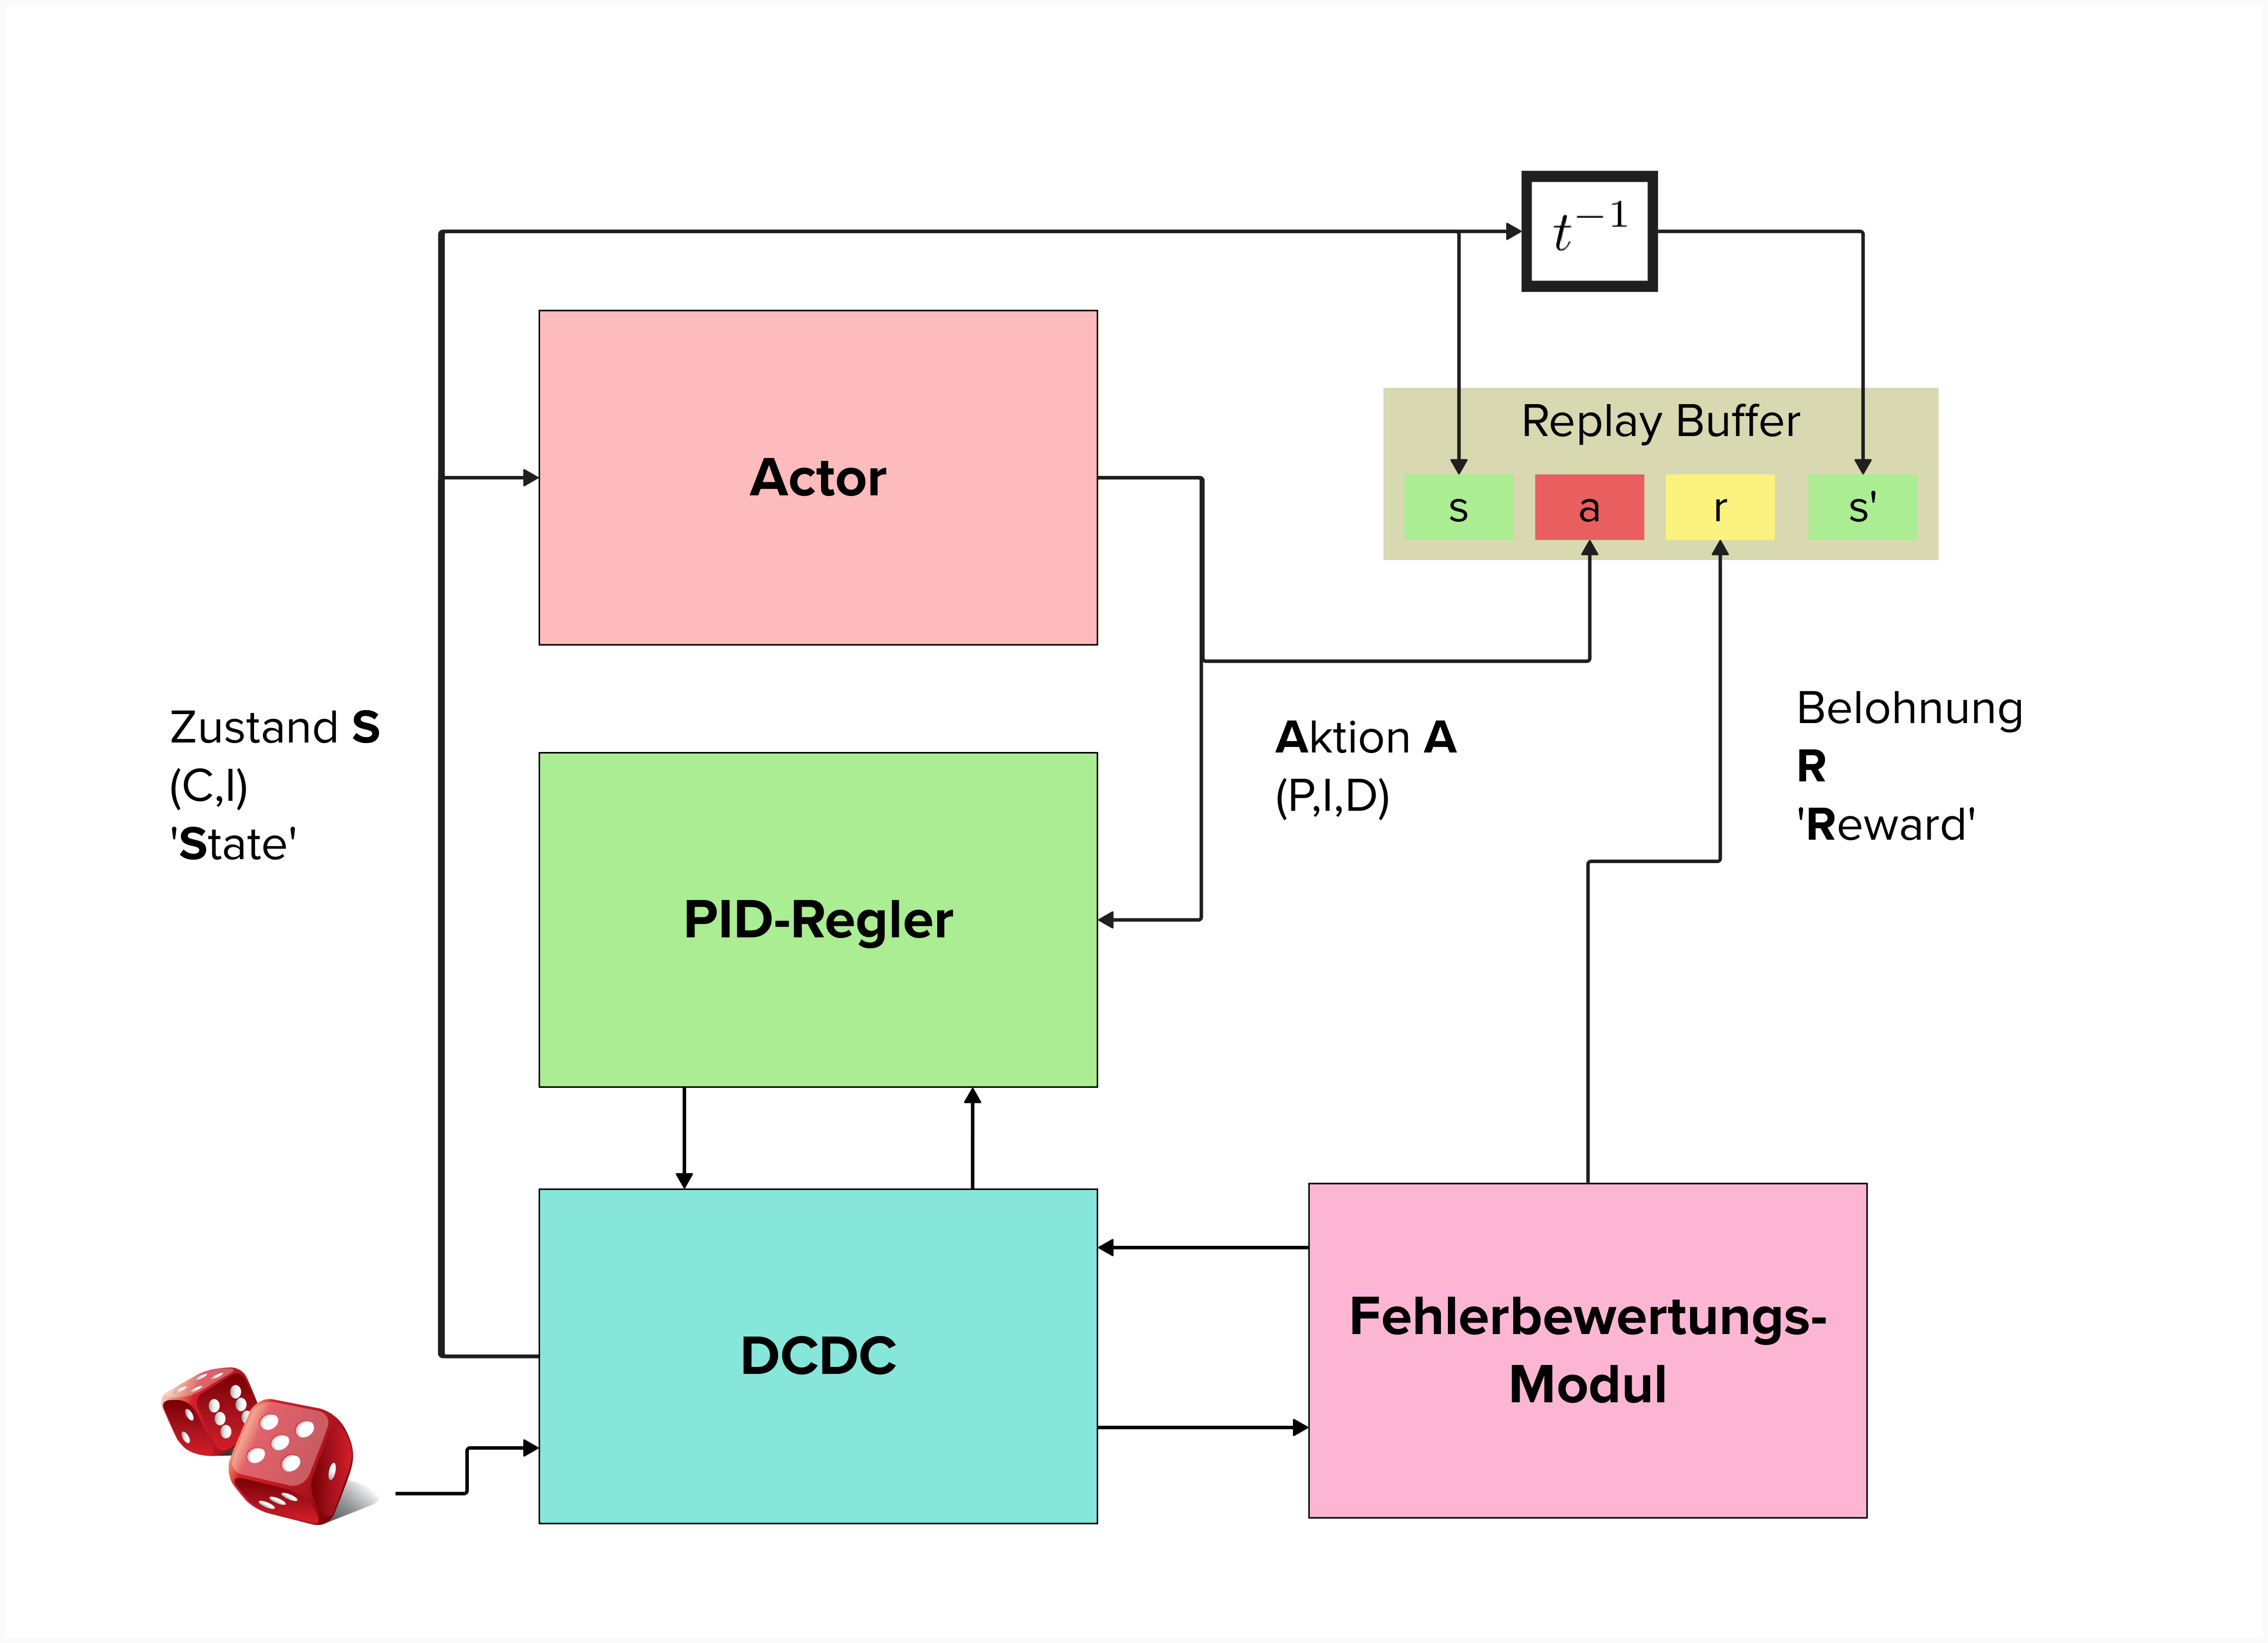
\includegraphics[width=0.72\textwidth]{3Experiment/2Experiment/0Experiment_Grob.png}
\caption{Detaillierte Darstellung des Systems zur Datensammlung für das Training des neuronalen Netzes.}
\label{fig:data_collection_system}
\end{figure}


\paragraph{Einleitung}
Dieser Abschnitt gewährt einen Überblick über die Struktur und den Datenfluss innerhalb Modueln\ref{fig:data_collection_system} Die detaillierten theoretischen Grundlagen der Systemkomponenten wurden im Grundlagenteil dieser Arbeit ausführlich behandelt. An dieser Stelle werden die Funktionen und Interaktionen der einzelnen Module im Kontext der Datenerfassung für das Training des neuronalen Netzes dargestellt.


\paragraph{Datenfluss im Reinforcement Learning System}
Im Zentrum des Datenflusses unseres Systems steht die Befüllung des Replay Buffers \ref{fig:replay_buffer}\ref{sec:Replay Buffers} mit wertvollen Informationen für das Training des Agenten. Diese Informationen bestehen aus den Zuständen der Schaltung, den getroffenen Aktionen des Agenten und den daraus resultierenden Belohnungen. 


\subsection{Makrozyklus: Systemüberblick und Datenauswertung}
Im Makrozyklus unseres Systems, wie in der beigefügten Abbildung \ref{fig:makrozyklus} dargestellt, konzentrieren wir uns auf die Simulation der Systemzustände und die anschließende Datenauswertung für das Training des neuronalen Netzwerks. Dieser Zyklus beinhaltet die Sammlung von Daten über verschiedene Zustände der Schaltung, einschließlich der Simulation der Systembedingungen sowie der Auswertung und Trainierung des neuronalen Netzwerks. Jeder Schritt in diesem Zyklus trägt dazu bei, ein umfassendes Verständnis der Systemdynamik zu entwickeln, was für die effiziente Anpassung des Netzwerks entscheidend ist. Der Makrozyklus wurde hauptsächlich in Python implementiert, um die Flexibilität und Erweiterbarkeit der Datenverarbeitungs- und Analyseprozesse zu maximieren.

\subsection{Mikrozyklus: Detailanalyse und Regelungsstrategien}

Im Mikrozyklus liegt der Fokus auf der Simulation der Verhaltensweisen des DC-DC-Konverters unter verschiedenen Bedingungen, insbesondere im Zusammenspiel mit einem PID-geregelten System. Diese Detailanalyse ermöglicht es, fein abgestimmte Regelungsstrategien zu entwickeln, die eine präzise Steuerung der Systemkomponenten unter variierenden Betriebsbedingungen erlauben. Der Mikrozyklus wurde in SystemC implementiert, was sich als besonders effizient für die Transientenanalyse einzelner Komponenten und die Simulation unter unterschiedlichen Bedingungen erwiesen hat. Die Durchführung eines Mikrozyklus auf einer Standard-CPU dauert etwa 0,3 Sekunden, was die schnelle Reaktionsfähigkeit und Anpassungsfähigkeit unseres Systems unterstreicht.

\begin{figure}[htbp]
\centering
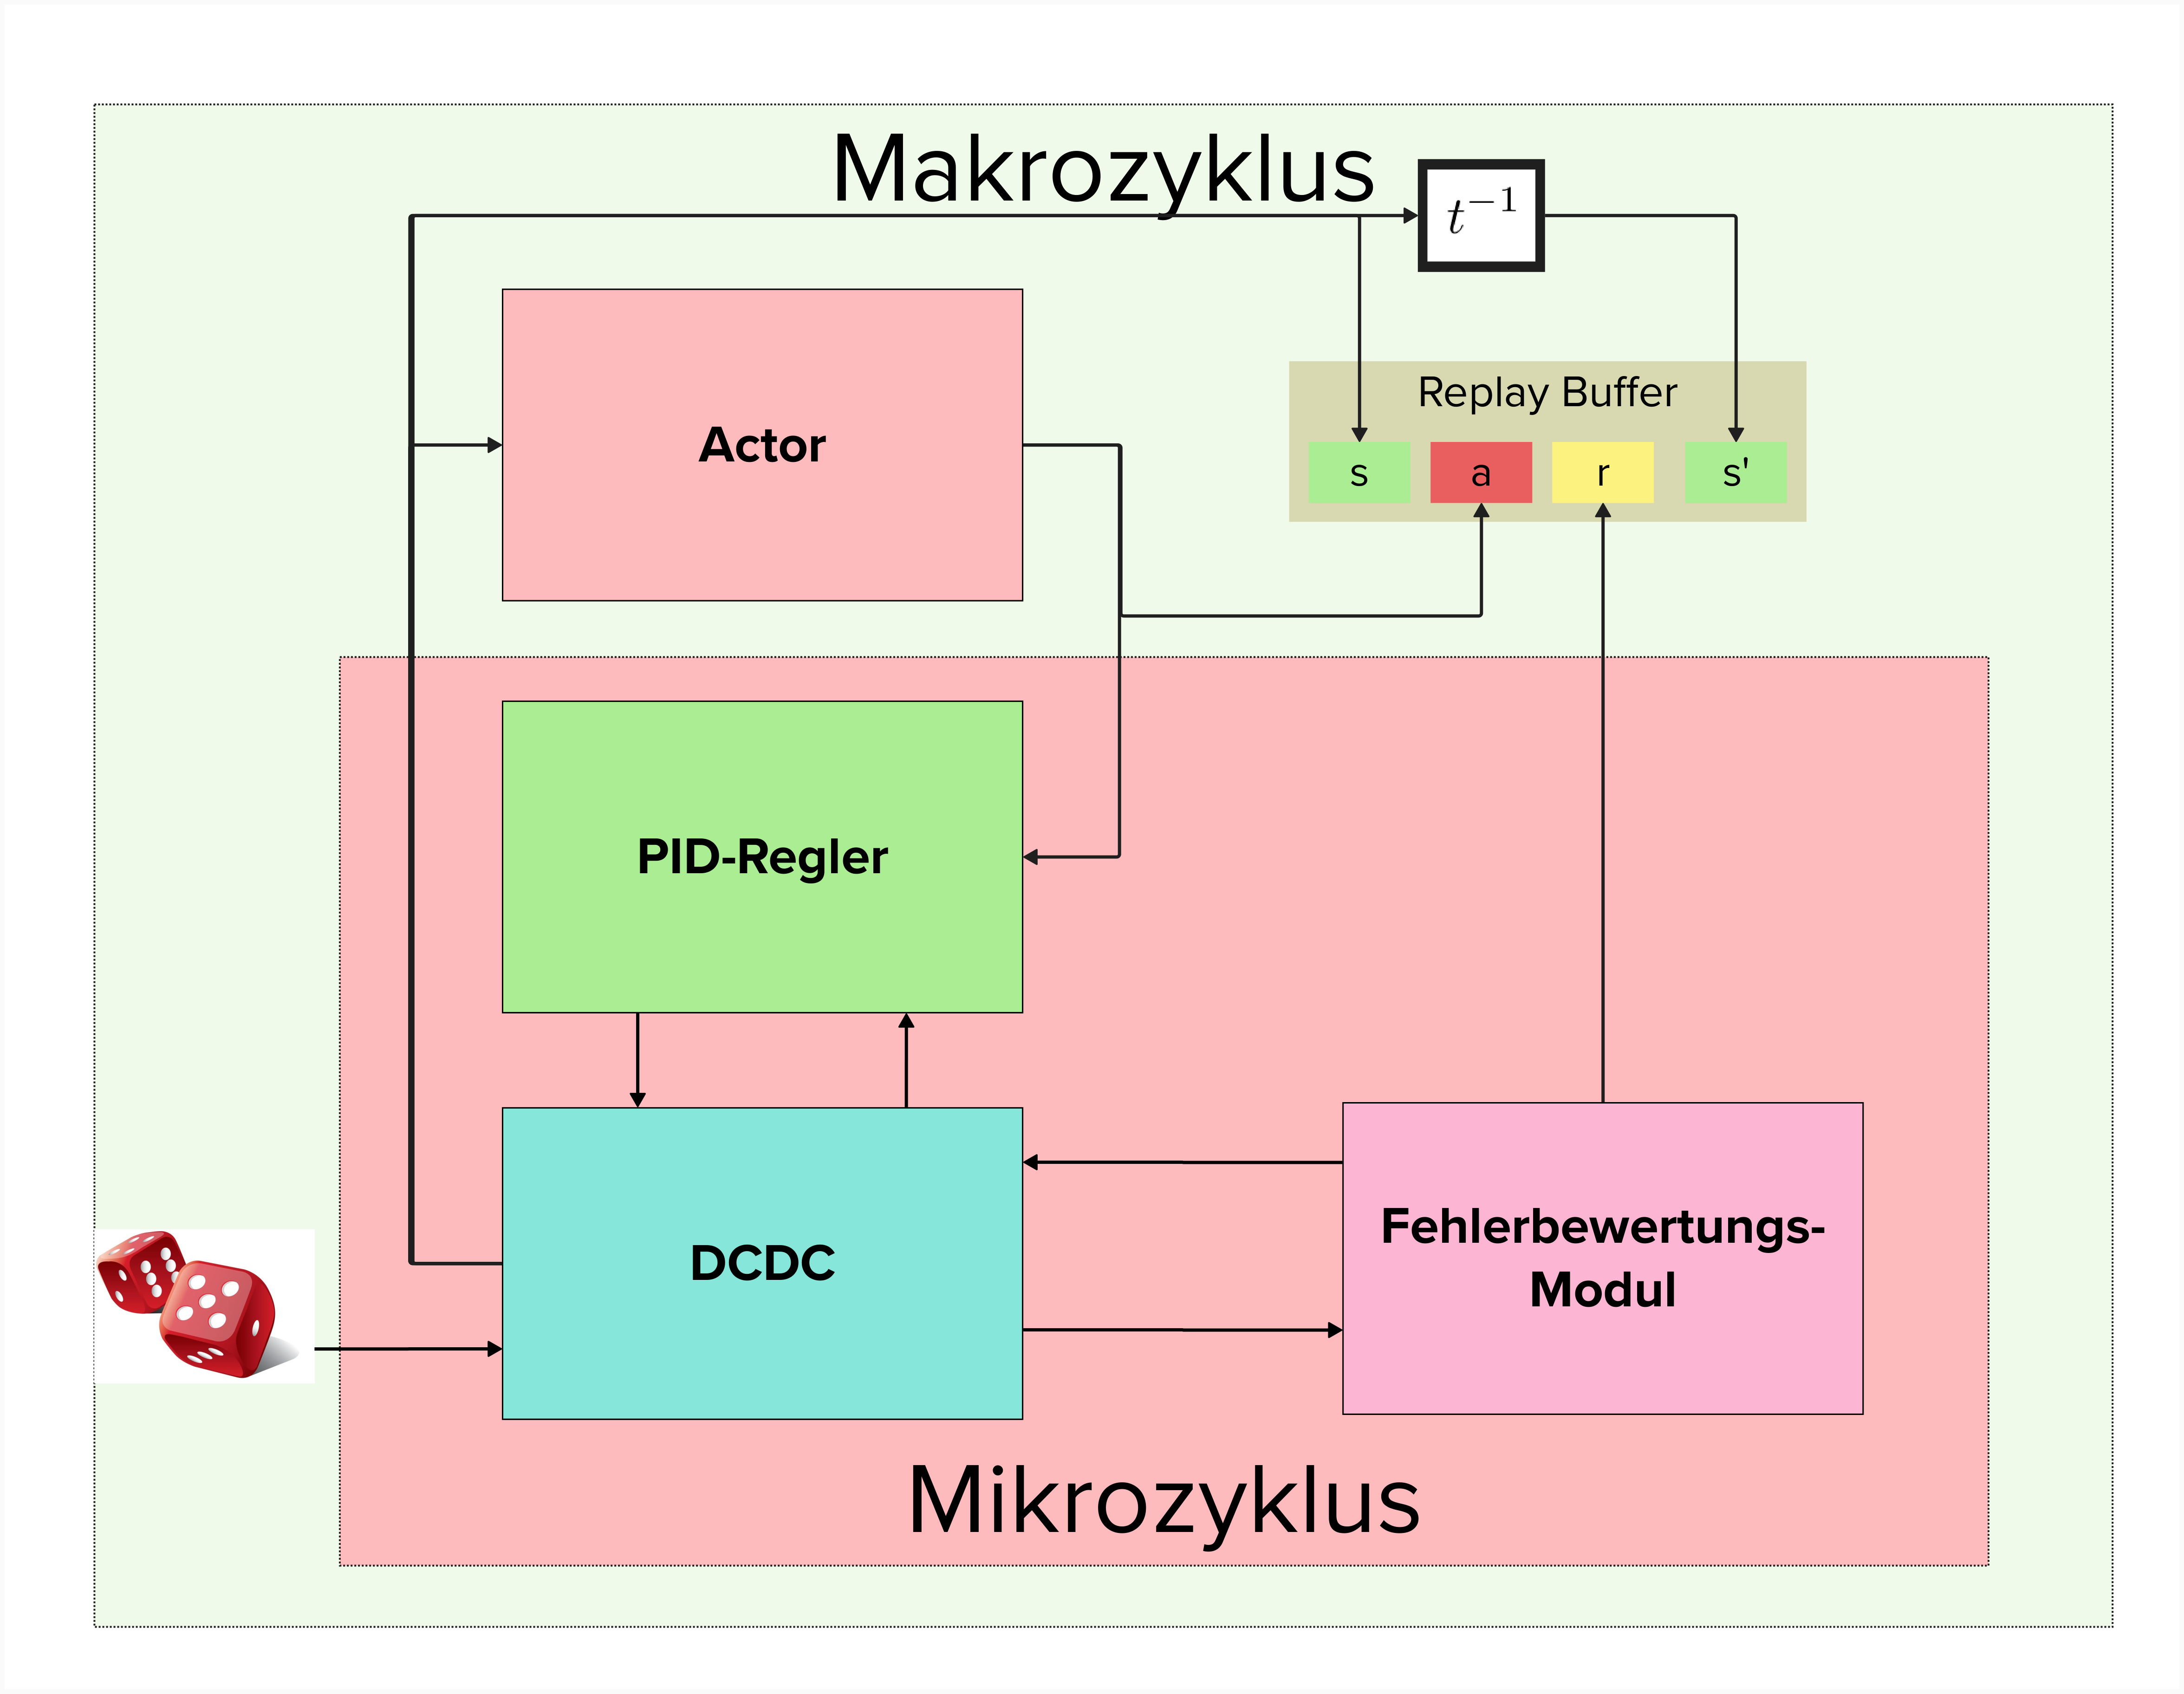
\includegraphics[width=0.8\textwidth]{3Experiment/2Experiment/0Zeitliche_Dimensio.png}
\caption{Visualisierung des Mikro- und Makrozyklus mit Darstellung der zeitlichen Unterteilung in zwei Dimensionen.}
\label{fig:makrozyklus}
\end{figure}




\begin{figure}[htbp]
\centering
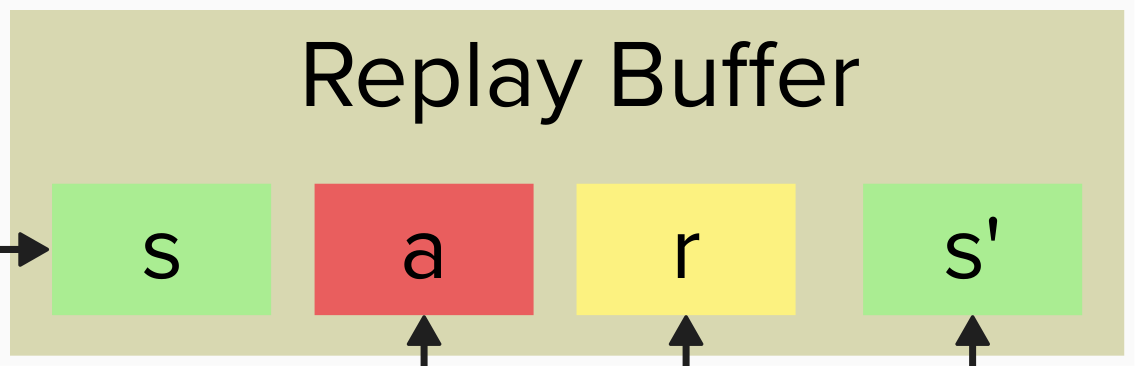
\includegraphics[width=0.4\textwidth]{3Experiment/2Experiment/0Replay_Buffer_short.png}
\caption{Schematische Darstellung des Replay Buffers, der als Datenspeicher für das Reinforcement Learning System dient. Er zeichnet die Sequenz der erlebten Zustände \( s \), Aktionen \( a \), Belohnungen \( r \) und nachfolgenden Zustände \( s' \) auf, welche für die stetige Anpassung und Verbesserung des Agenten verwendet werden.}
\label{fig:replay_buffer}
\end{figure}

\subsection{ Makrozyklus Schritt 1: Zustandssimulation und Datengenerierung}

Die Generierung der Schaltungszustände, die als Input für den Lernprozess dienen, erfolgt mittels einer Zufallsfunktion. In der realen Welt erfolgen Zustandsübergänge in einer physischen Schaltung in langen Zeitintervallen, was eine direkte Simulation unpraktisch macht. Deshalb greifen wir auf eine alternative Methode zurück:

\begin{itemize}
    \item Initial wird über eine Gleichverteilung ein Degenerationszustand der Schaltung simuliert. Die zufällige Auswahl dieser Zustände geschieht innerhalb festgelegter Grenzen, um eine Vielfalt an möglichen Zuständen zu gewährleisten.
	\item Der simulierte Zustand wird durch einen Satz von Kapazitäts- und Induktivitätswerten dargestellt. Diese Werte werden durch den "Würfel" im System visualisiert \ref{fig:state_generation}, wobei die Pfeile vom Würfel zu den Zustandsvariablen C und L diesen Prozess der zufälligen Zustandsgenerierung abbilden.
\end{itemize}

In diesem Projekt werden exemplarische Einstellungen für die Zustandsgenerierung verwendet, die eine Annäherung an realitätsnahe Bedingungen darstellen. Bei einer Überführung in praktische Anwendungen würden diese Einstellungen so angepasst, dass sie mit den in der Realität verifizierten Werten übereinstimmen. Die aktuellen Grenzwerte für die Zustandsgenerierung sind wie folgt definiert:

\begin{itemize}
    \item Untergrenze: \( \text{Induktivität} = 5.0 \times 10^{-4} \), \( \text{Kapazität} = 1.0 \times 10^{-6} \)
    \item Obergrenze: \( \text{Induktivität} = 5.0 \times 10^{-2} \), \( \text{Kapazität} = 1.0 \times 10^{-4} \)
\end{itemize}

\begin{figure}[htbp]
\centering
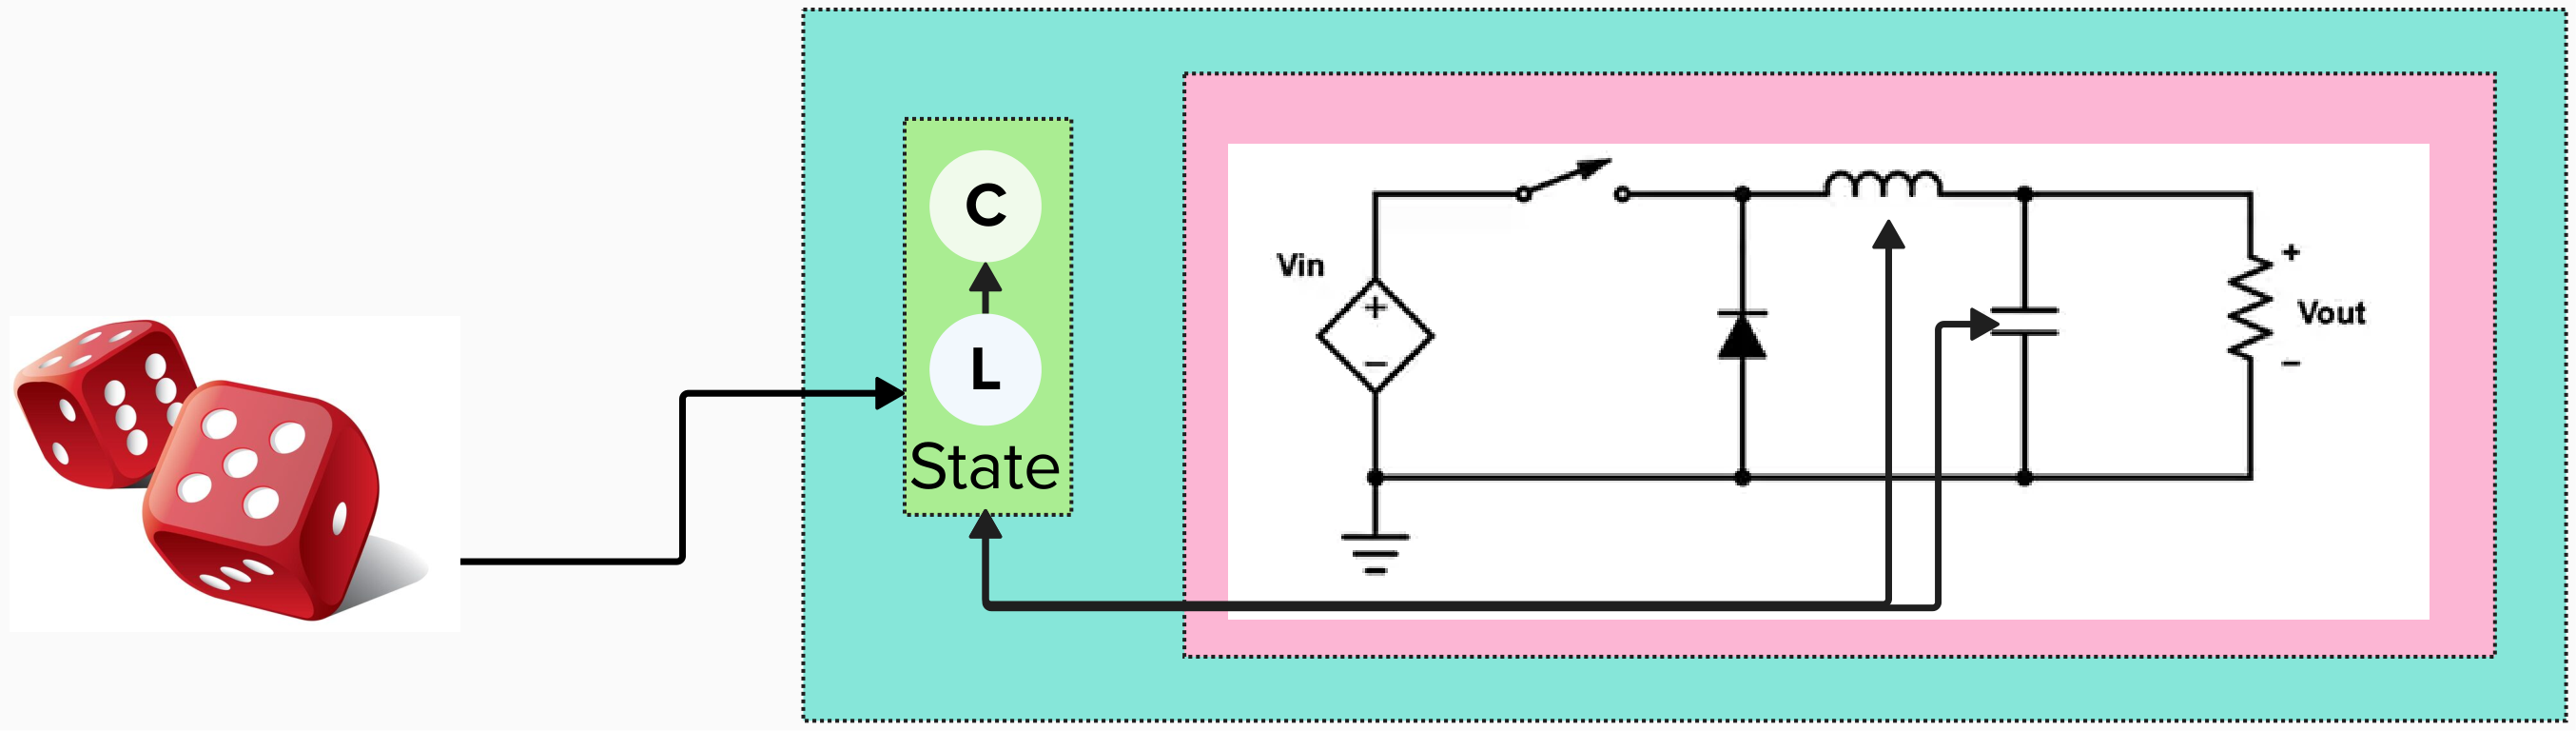
\includegraphics[width=0.7\textwidth]{3Experiment/2Experiment/1Random_Set_State.png}
\caption{Visualisierung der Zustandsgenerierung mit dem Würfel und die Setzung der Werte in der DCDC-Schaltung.}
\label{fig:state_generation}
\end{figure}

\subsection{Makrozyklus Schritt 2: Entscheidungsfindung durch den Actor}

Nachdem der initiale Schaltungszustand durch eine Zufallsverteilung generiert wurde, kommt der Actor ins Spiel, der auf Basis der aktuellen Kapazitäts- (C) und Induktivitätswerte (L) Entscheidungen trifft. Der Actor, ein wesentlicher Bestandteil des Reinforcement Learning Systems, ist eine komplexe Funktion, die sich aus mehreren Gewichtungen (weights) und Verzerrungen (biases) zusammensetzt. Diese werden im Laufe des Vorwärtsdurchlaufs (Forward Propagation \ref{sec: Forward Propagation}) durch das Netzwerk multipliziert und summiert.

\begin{itemize}
		\item Innerhalb des Actors wird die Eingabe durch jede Schicht des neuronalen Netzwerks transformiert, wobei nach jedem Schichtdurchgang eine nicht-lineare Aktivierungsfunktion \ref{eq:activation_function} angewandt wird, um die Linearität der Operationen zu durchbrechen.
		\item Im spezifischen Kontext unseres Systems ist die Aktivierungsfunktion der letzten Schicht eine  Hyperbelfunktion (tanh), die die Ausgabe des Netzwerks beeinflusst und zu einem komplexen, nicht-linearen Ergebnis führt.
\end{itemize}

Die Ausgabe des Actors sind die PID-Werte, die für die Steuerung des nächsten Schrittes im System verwendet werden. Diese Werte sind das Resultat des durch die tanh-Funktion modifizierten Outputs und stellen somit eine fein abgestimmte Reaktion auf den Zustand der Schaltung dar. Diese Werte werden anschließend skaliert, um realistische PID-Reglerparameter zu erhalten:

\begin{itemize}
	\item Der Proportionalwert (Kp) wird zwischen 0 und 10 skaliert.
	\item Der Integralwert (Ki) wird zwischen 0 und 1 skaliert.
	\item Der Differentialwert (Kd) wird zwischen 0 und 0.1 skaliert.
\end{itemize}

Diese Skalierung ist entscheidend, um die Ausgangswerte des neuronalen Netzes in praktikable Steuerparameter zu überführen. Die Transformation gewährleistet, dass die PID-Werte in einem Bereich liegen, der für die Regelung des Systems adäquat ist und reflektiert die praktischen Anforderungen an die Systemsteuerung. 


\begin{figure}[htbp]
\centering
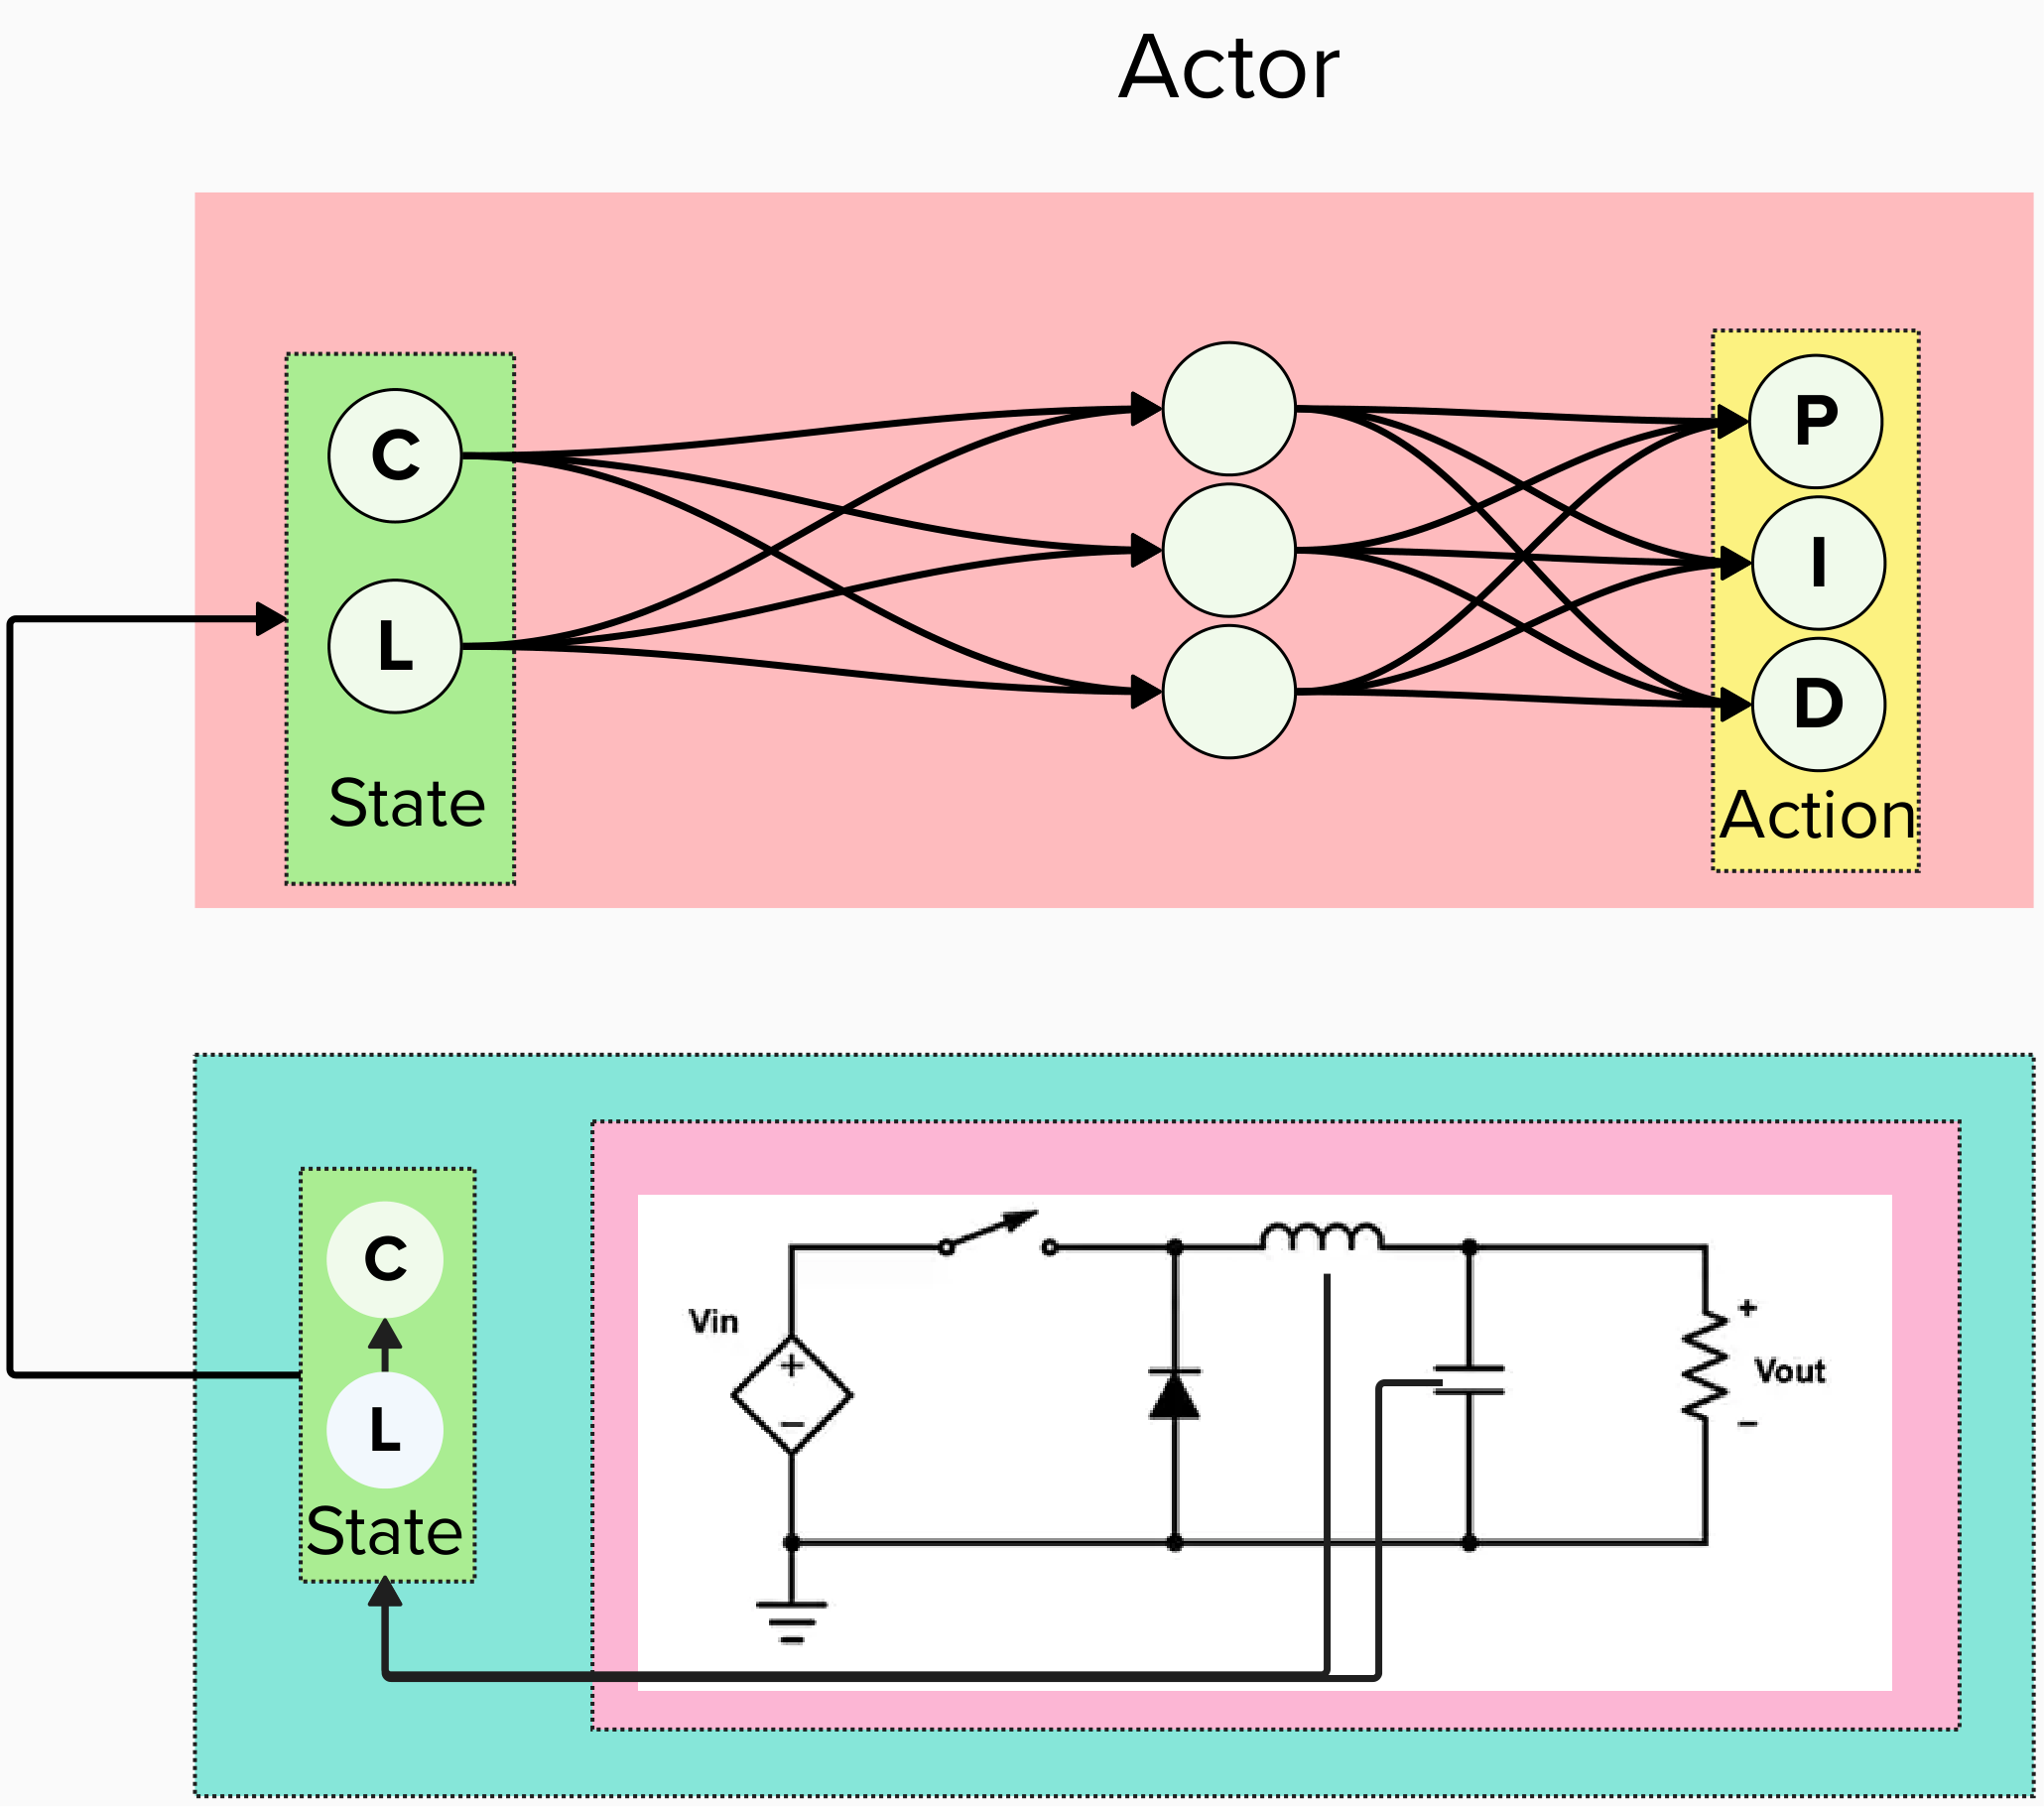
\includegraphics[width=0.5\textwidth]{3Experiment/2Experiment/2Actor.png}
\caption{Die Forward Propagation im Actor-Modul, die den Zustand S (C, L) aufnimmt und über ein mehrschichtiges neuronales Netzwerk PID-Aktionswerte ausgibt.}
\label{fig:actor_decision_making}
\end{figure}




\subsection{Gesamtdarstellung des Regelkreises mit PID-gesteuertem DCDC-Konverter}
\label{sec:Gesamtdarstellung_Regelkreis}

Dieser Abschnitt bietet einen umfassenden Überblick über den Regelkreis, der einen PID-Regler, einen Pulsweitenmodulator (PWM) und einen DCDC-Konverter umfasst. Im Mittelpunkt steht die Interaktion dieser Komponenten, die gemeinsam eine konstante Ausgangsspannung gewährleisten. Die Mikroebene der Simulation wird besonders hervorgehoben, um die Auswirkungen der Wechselwirkungen zwischen den einzelnen Elementen auf die Gesamtleistung des Systems zu verdeutlichen.
Abbildung \ref{fig:Regelkreis_Überblick} veranschaulicht den gesamten Regelkreis inklusive des PID-gesteuerten DCDC-Konverters.

\paragraph{Interaktion der Regelkreiskomponenten}
Der Regelungsprozess beginnt mit den vom Actor gelieferten PID-Koeffizienten \( K_p, K_i, \) und \( K_d \), die den PID-Regler ansteuern (siehe Abschnitt \ref{sec:PID-Regler}). Der Regler vergleicht kontinuierlich die aktuelle Spannung mit dem Referenzwert und generiert ein Signal zur Korrektur, das an den PWM weitergeleitet wird.

\paragraph{Funktionsweise des Pulsweitenmodulators (PWM)}
Der PWM-Modulator (Abschnitt \ref{sec:PWM_Grundlagen}) transformiert das Signal des PID-Reglers in eine pulsbreitenmodulierte Form, die den DCDC-Konverter ansteuert. Dieser Konverter sorgt für die Umwandlung der Eingangsspannung in eine stabile Ausgangsspannung. Die Signalverarbeitung im PWM bestimmt die Schaltfrequenz des Transistors im Konverter, um die Last angemessen zu versorgen.

\paragraph{Rolle des DCDC-Konverters}
Der DCDC-Konverter spielt eine zentrale Rolle im Regelkreis, indem er die Energie der Versorgungsspannung in eine nutzbare Ausgangsspannung umwandelt(siehe Abschnitt \ref{sec:DCDC_Konverter}) . Die Arbeitsweise des Konverters ist eng mit den PWM-Signalen verknüpft, welche das Öffnen und Schließen des Transistors steuern. Die PWM regelt die Impulsbreite basierend auf den Steuerbefehlen des PID-Reglers. Diese Impulse beeinflussen das Tastverhältnis und damit die Energiemenge, die durch den Transistor geleitet wird. Die Energie wird in der Induktivität gespeichert und als Strom an die Last abgegeben, wobei die Kapazität als Puffer dient. Änderungen in der Last führen zu Spannungsschwankungen, die der PID-Regler erfasst und ausgleicht, um eine stabile Ausgangsspannung zu gewährleisten.

\paragraph{Integration von Simulation und Realität}
Die Simulation des Regelkreises erfolgte in SystemC, wobei der PID-Regler direkt aus mathematischen Modellen abgeleitet und der PWM sowie der DCDC-Konverter für eine genauere Analyse implementiert wurden. Dies ermöglicht einen Ausgleich zwischen Genauigkeit und Simulationsgeschwindigkeit.


\begin{figure}[htbp]
    \centering
    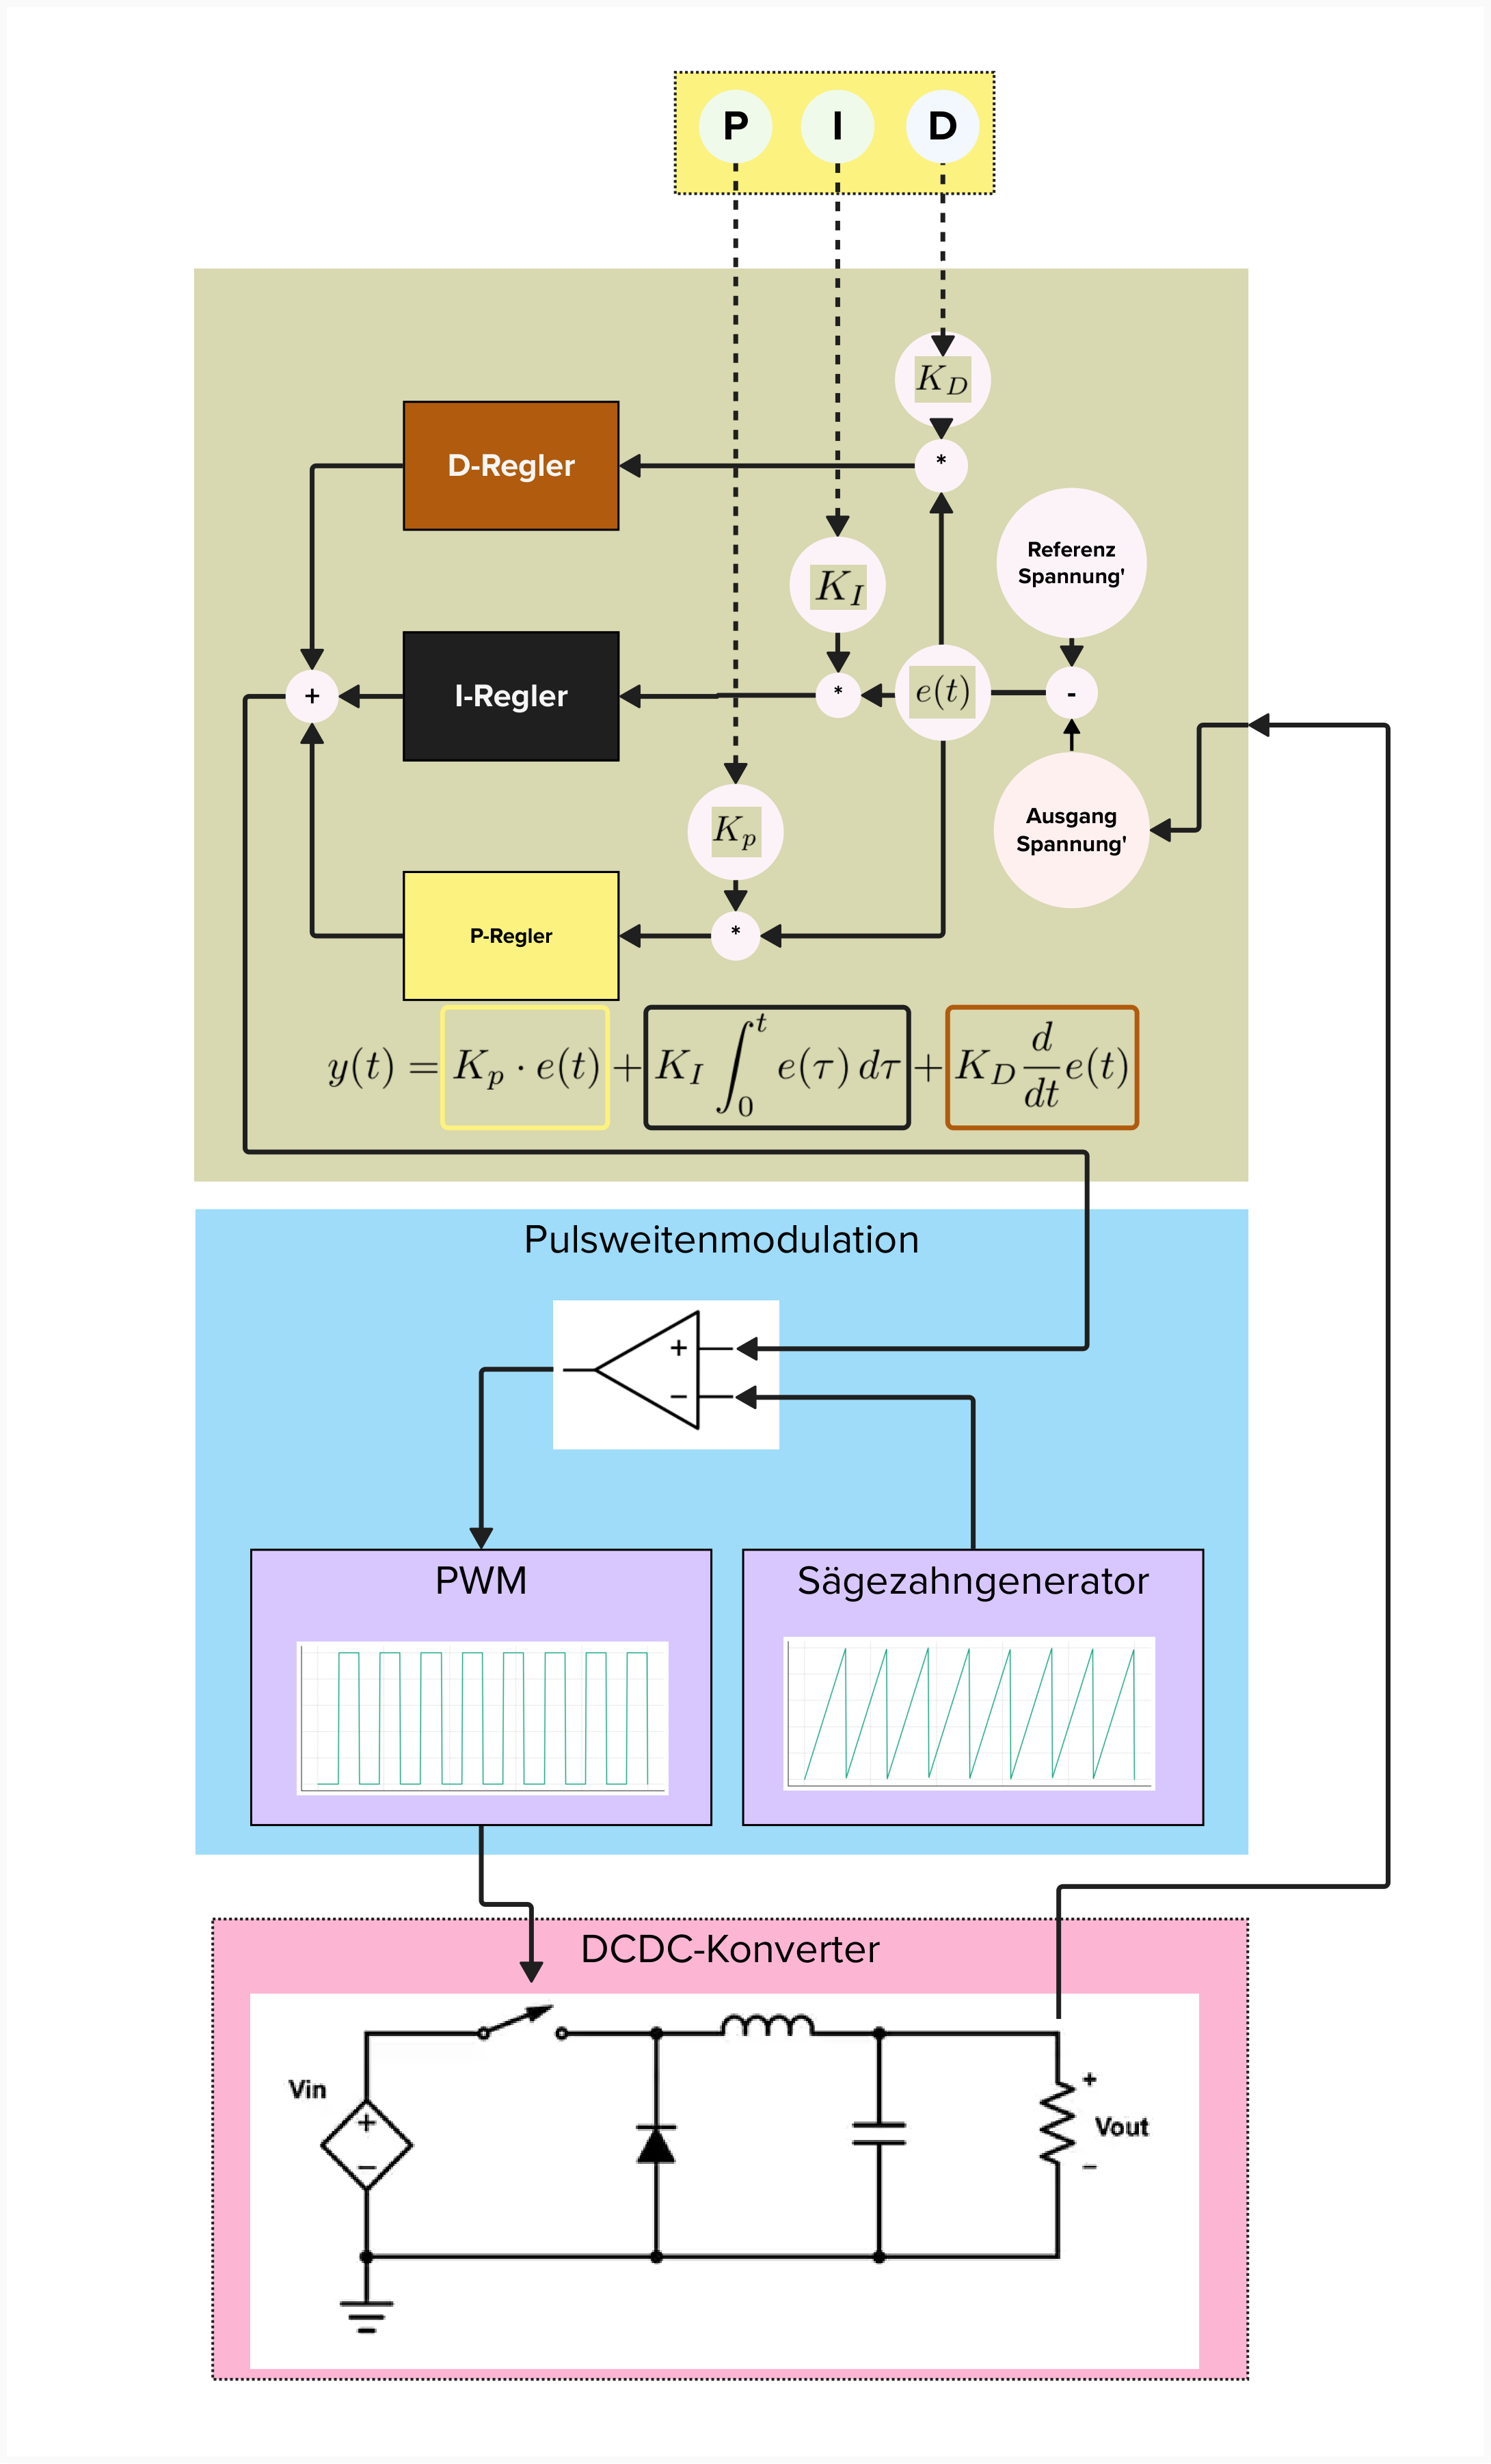
\includegraphics[width=0.99\linewidth]{3Experiment/2Experiment/3PID_Gesteuerter_DCDC_Converter.png}
    \caption{Überblick über den Regelkreis mit dem PID-Regler, PWM und DCDC-Konverter.}
    \label{fig:Regelkreis_Überblick}
\end{figure}

\subsection{Selbsttestmodul im Lernprozess des Agenten}
\label{sec:Selbsttestmodul}

Das Selbsttestmodul ist ein essentielles Element unserer Systemarchitektur, welches die Schnittstelle zwischen Theorie und Praxis repräsentiert. Es bewertet und optimiert die Effektivität der vom Agenten erlernten Schaltstrategien.

\paragraph{Funktion und Notwendigkeit des Selbsttests}
Der Selbsttest bewertet die Schaltungsreaktionen auf definierte Testszenarien, um die Lernergebnisse des Agenten zu überprüfen, wie in Abbildung \ref{fig:RewardOverTime} dargestellt.
\begin{figure}[htbp]
    \centering
    
\includegraphics[width=0.5\linewidth]{3Experiment/2Experiment/4reward.png}
    \caption{Darstellung des Selbsttestmoduls im Regelkreis mit PID-Regler, PWM und DCDC-Konverter.}
    \label{fig:ControlLoop}
\end{figure}

\paragraph{Methodik der Performanzbewertung}
Die Bewertungsmethodik integriert die Abweichungen zwischen Soll- und Ist-Spannung, wobei größere Fehler durch Quadrierung stärker gewichtet werden. Extreme Spannungsspitzen werden, wie in Abbildung \ref{fig:CumulativeReward} gezeigt, exponentiell bestraft.
\begin{figure}[htbp]
    \centering
    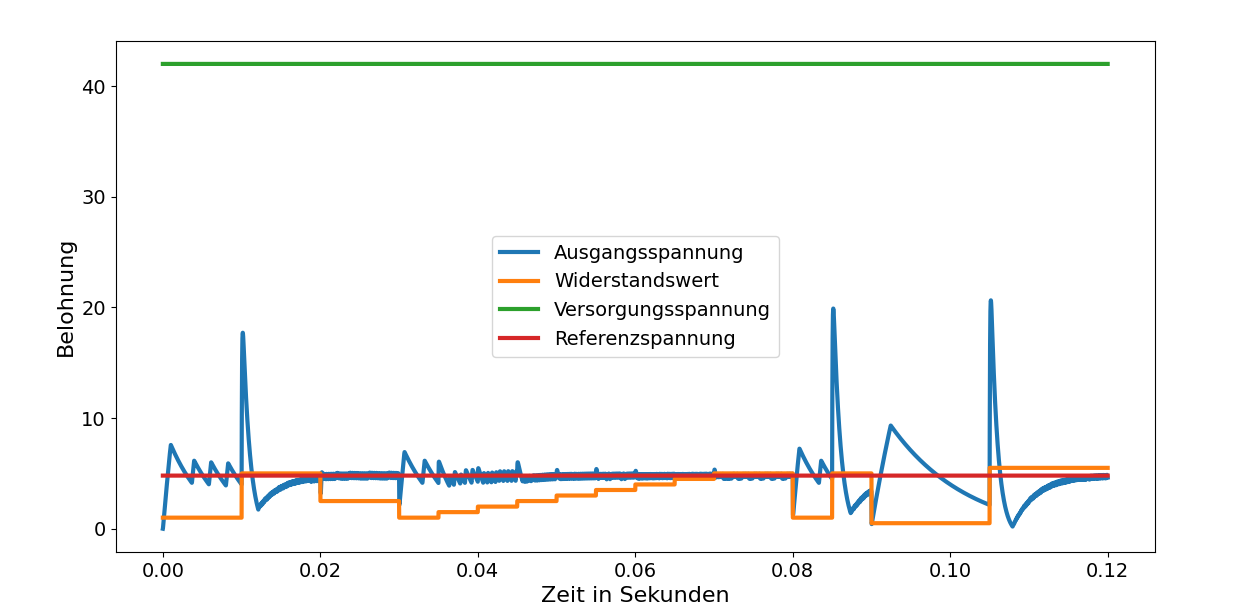
\includegraphics[width=0.99\linewidth]{3Experiment/2Experiment/4Reard_over_time.png.png}
    \caption{Visualisierung des Rewards über die Zeit während der Simulation.}
    \label{fig:RewardOverTime}
\end{figure}
\begin{figure}[htbp]
    \centering
    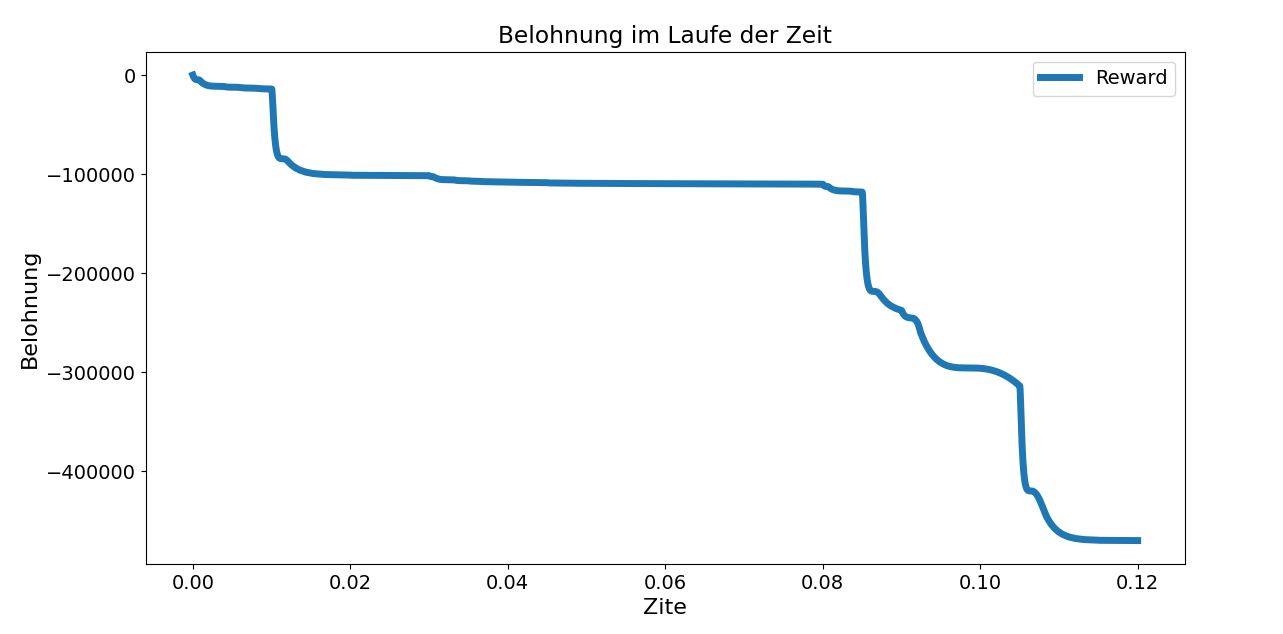
\includegraphics[width=0.99\linewidth]{3Experiment/2Experiment/4Cumulativer_Reward_Uber_Zeit.png.png}
    \caption{Kumulativer Reward über die Zeit, aufgezeichnet während der Systemtests.}
    \label{fig:CumulativeReward}
\end{figure}

\paragraph{Auswirkungen auf das Trainingsziel}
Diese Bewertungsmethodik führt zu einem quantifizierbaren Wert, der die Qualität der Regelung anzeigt und den Agenten anleitet, den Fehlerwert zu minimieren. Dies wird durch den negativen Reward widergespiegelt, der in den Lernprozess des Agenten einfließt.

\paragraph{Zeitliche Dimension der Analyse}
Selbsttests werden in wiederkehrenden Zyklen durchgeführt und bewertet, wobei der kumulierte Fehlerwert im Replay Buffer gespeichert wird, um die Strategie zu optimieren, wie in Abbildung \ref{fig:makrozyklus} illustriert.


\section{Zusammenführung des Actor-Critic-Verfahrens}
\label{sec:Synthesis_Actor_Critic}

Im vorherigen Kapitel haben wir eine Trainingsumgebung für verstärkendes Lernen etabliert, die das Sammeln von Zuständen, Aktionen und Belohnungen (Rewards) umfasst. Diese Daten werden in einem Replay Buffer gespeichert, aus dem sie entsprechend der Batch-Größe  für das Training entnommen werden.(siehe Abschnitt \ref{sec: Batch})

\paragraph{Die Dynamik des Replay Buffers}
Aus dem Replay Buffer (siehe Abschnitt  \ref{sec:Replay Buffers}) werden Datensätze extrahiert, die simultan zur Berechnung des Gradienten und zur Aktualisierung der Actor-Critic Architektur herangezogen werden.
Der Replay Buffer ist das Herzstück unserer Trainingsdynamik. Er speichert die Erfahrungen, die der Algorithmus im Laufe der Simulation macht, und ermöglicht es uns, die komplexen Zusammenhänge zwischen Aktionen und resultierenden Belohnungen zu extrahieren.

\paragraph{Die Aufgabe des Critics}
Der Critic bewertet die vom Actor ausgeführte Policy und den gegebenen Zustand,evaluiert die Effektivität der vom Actor vorgeschlagenen Aktionen im Kontext der Schaltung ( siehe Abschnitt \ref{eq:critick update}). Die generierten Schätzwerte des Critics werden mit den tatsächlichen Belohnungen verglichen, womit der Critic das Verhalten der Schaltung in Abhängigkeit von der jeweiligen Konfiguration prognostiziert. Der Critic  Durch das Abgleichen seiner Vorhersagen mit den tatsächlichen Belohnungen lernt der Critic, das Verhalten der Schaltung präzise vorherzusagen und unterstützt damit die zielgerichtete Anpassung der PID-Koeffizienten.

\paragraph{Optimierungsmechanismus des Actors}
Die Feinjustierung des Actors ist ein zentraler Bestandteil des Lernprozesses innerhalb der Actor-Critic Architektur. Anstatt komplexe Bewertungen vorzunehmen, wird ein Gradient berechnet, der die Gewichte des Actors so anpasst, dass die Schätzung des Critics in die richtige Richtung gelenkt wird, um den Reward zu maximieren (siehe Abschnitt \ref{eq:actor update}). Dieser Ansatz ermöglicht es dem Actor, aus den Prognosen des Critics zu lernen und seine Policy systematisch so zu verfeinern, dass die Belohnungsausschüttung erhöht wird. Es handelt sich hierbei um den Kern des Lernvorgangs, bei dem der Actor durch die Adjustierung seiner Gewichte basierend auf der Kritik und den Belohnungen iterativ verbessert wird.

\begin{figure}[htbp]
    \centering
		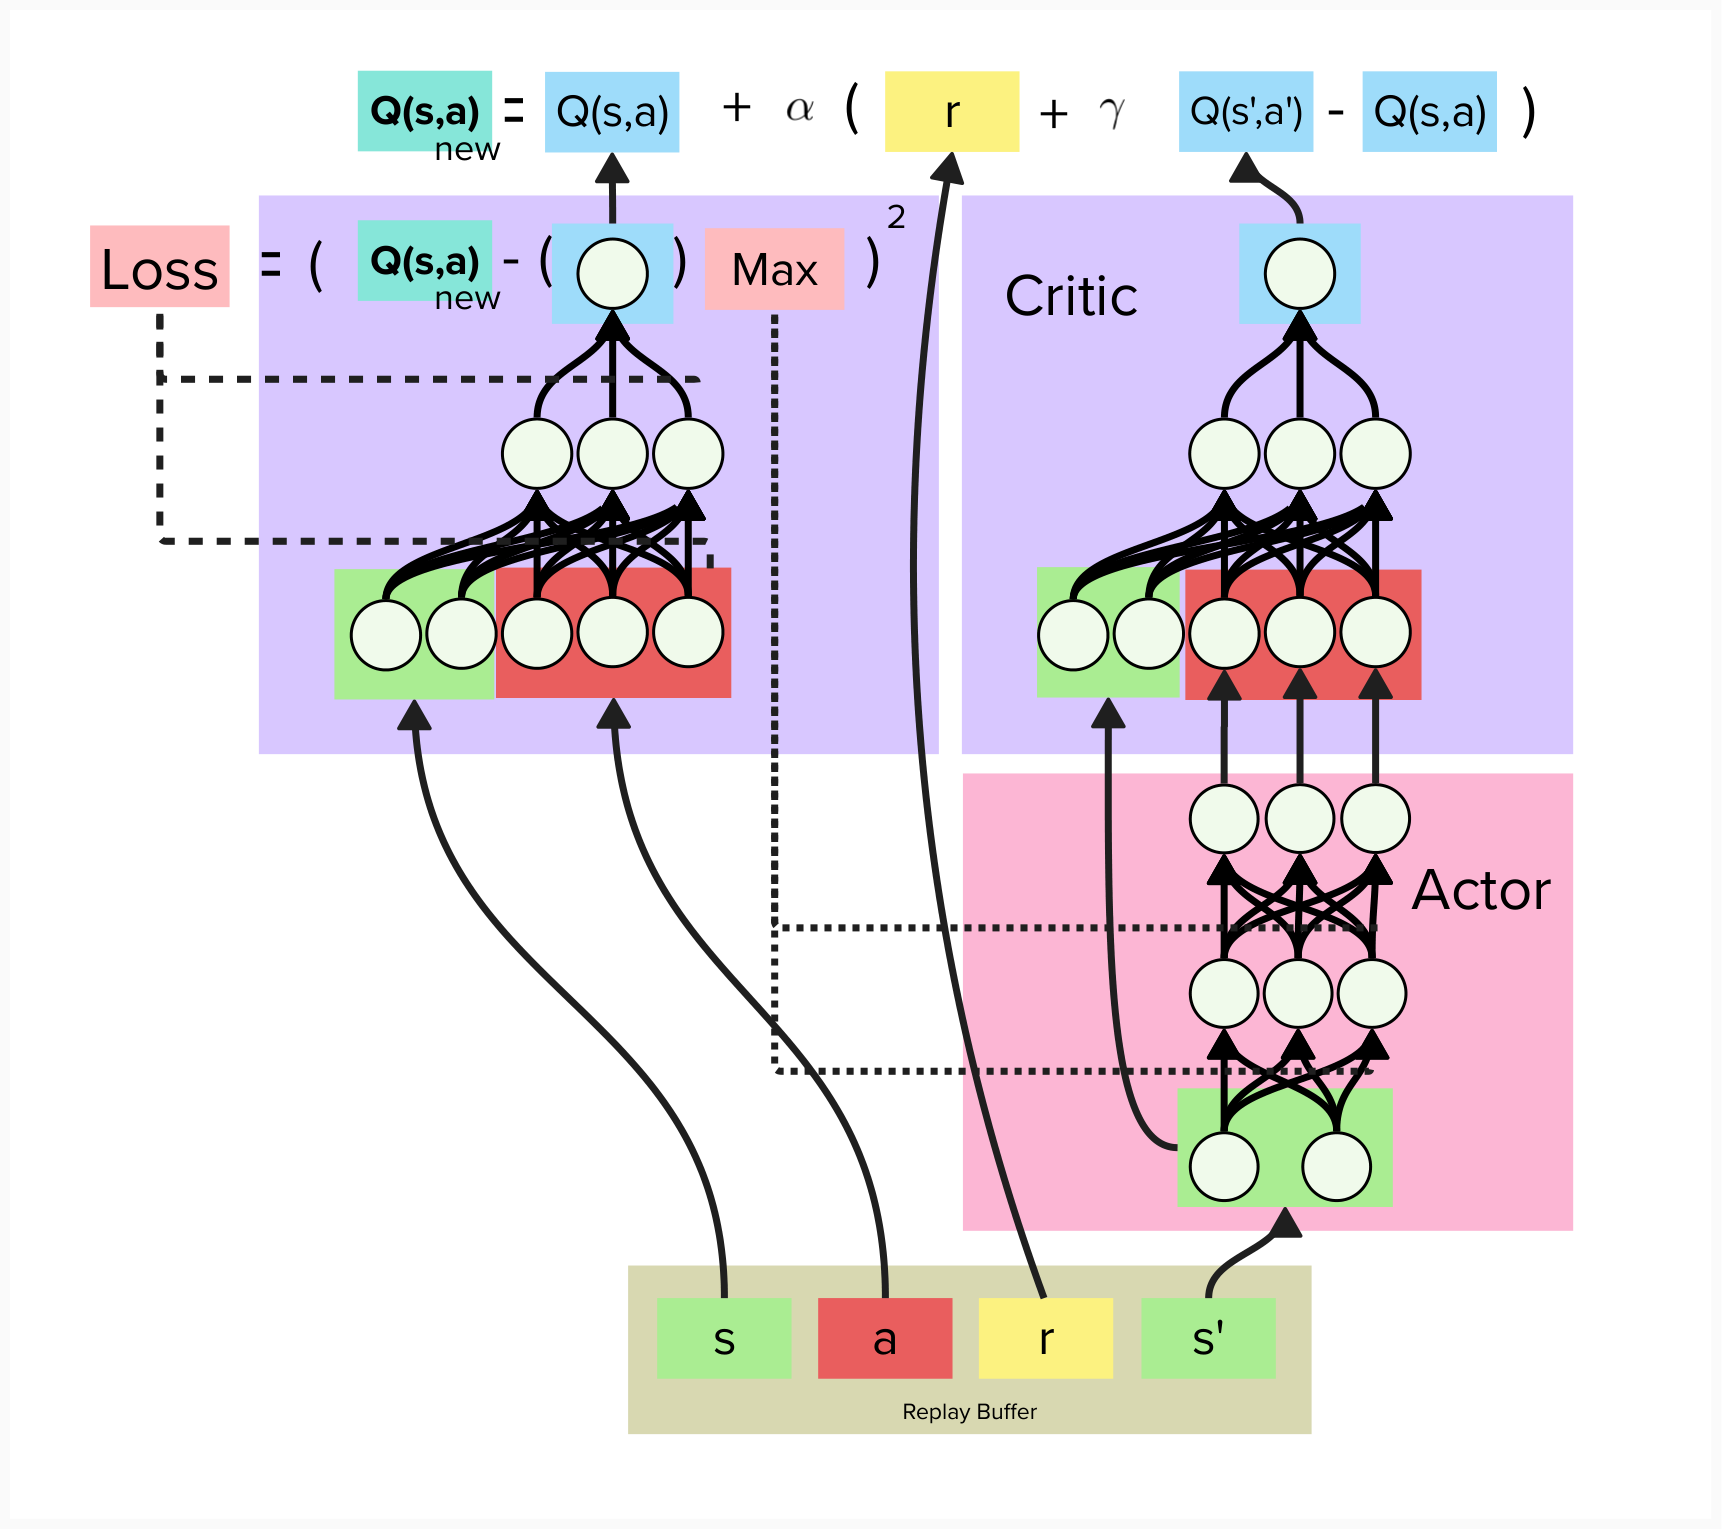
\includegraphics[width=\linewidth, trim=10px 10px 10px 10px, clip]{3Experiment/2Experiment/5Actor_Critick.png}
    \caption{Zusammengefasste Visualisierung des Update-Prozesses in der Actor-Critic Architektur.}
    \label{fig:ActorCriticSynthesis}
\end{figure}


\paragraph{Kontinuierliche Verbesserung durch Training}
Die stetige Aktualisierung des Gradienten nach jedem Simulationsschritt sorgt für eine kontinuierliche Anpassung und Verfeinerung der Actor-Critic Architektur (siehe Abschnitt \ref{sec:Synthesis_Actor_Critic}), was die Belohnungen im Laufe der Zeit maximiert. Angenommen, das Ziel ist eine direkte Optimierung der Belohnungen in unserer Simulation – die Herausforderung besteht darin, dass die komplexe Pipeline von Aktionen bis hin zum endgültigen Reward nicht mit einfachen mathematischen Mitteln abgebildet werden kann. Daher nutzen wir den Actor-Critic Ansatz, um einen einfacheren Gradienten in Bezug auf den erwarteten Reward zu maximieren, was indirekt die Optimierung der Aktionen ermöglicht.


 


% \subsection{Aufbau des Replay Buffers und Sammlung von Trainingsdaten}

Ein kritischer Schritt im Trainingsprozess des neuronalen Netzes ist die Befüllung des Replay Buffers \ref{sec:Replay Buffers}. Der Replay Buffer ist ein Speichermechanismus, der die Interaktionen des Agenten mit der Umgebung festhält, um daraus zu lernen. Er speichert Tupel \( (s, a, r, s') \), bestehend aus dem aktuellen Zustand \( s \), der vom Actor gewählten Aktion \( a \), der daraus resultierenden Belohnung \( r \) und dem nachfolgenden Zustand \( s' \).

\begin{figure}[htbp]
\centering
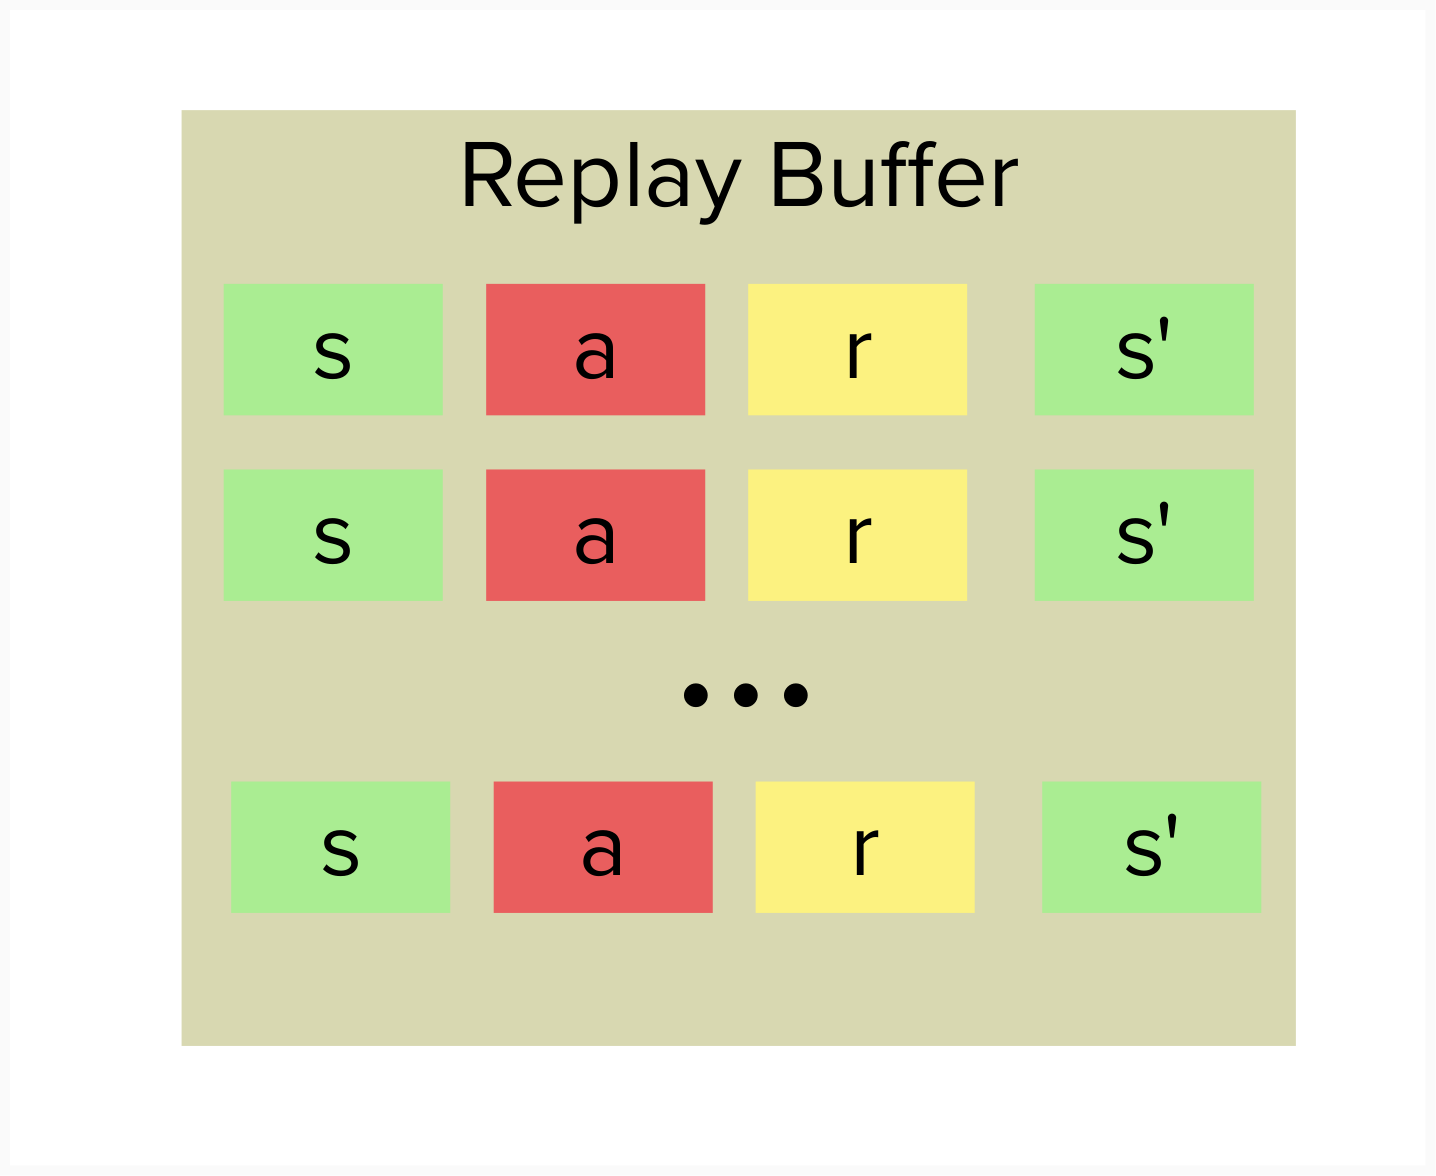
\includegraphics[width=0.5\textwidth]{3Experiment/2Experiment/1Replay_Buffer.png}
\caption{Schematische Darstellung des Replay Buffers, der die Elemente \( s \), \( a \), \( r \), und \( s' \) speichert, welche die Zustände, Aktionen, Belohnungen und Folgezustände repräsentieren.}
\label{fig:replay-buffer}
\end{figure}

Die im Replay Buffer \ref{fig:replay-buffer} gespeicherten Daten werden für das Training des neuronalen Netzes verwendet.












% \section{Ergebnisse}
% \section{Diskussion}
% \section{Schlussfolgerungen und Ausblick}




%^#### 3. Technische Umsetzung / Implementierung und Software-Architektur
%^- Programmiersprachen und Bibliotheken
%^  - C++
%^  - TensorFlow
%^  - Python
%^  - SystemC

%^- Schnittstellen-Design
%^  - API-Entwicklung
%^  - Modulare Architektur

%^- SystemC in der Schaltungssimulation
%^  - Grundlagen
%^  - Transientenanalyse
%^  - Vorteile und Herausforderungen
%^- Implementierungsdetails
%^  - Code-Architektur
%^  - Optimierung für Performanz


\chapter{Ergebnisse}

% \subsection{ Makrozyklus Schritt 1: Zustandssimulation und Datengenerierung}

Die Generierung der Schaltungszustände, die als Input für den Lernprozess dienen, erfolgt mittels einer Zufallsfunktion. In der realen Welt erfolgen Zustandsübergänge in einer physischen Schaltung in langen Zeitintervallen, was eine direkte Simulation unpraktisch macht. Deshalb greifen wir auf eine alternative Methode zurück:

\begin{itemize}
    \item Initial wird über eine Gleichverteilung ein Degenerationszustand der Schaltung simuliert. Die zufällige Auswahl dieser Zustände geschieht innerhalb festgelegter Grenzen, um eine Vielfalt an möglichen Zuständen zu gewährleisten.
	\item Der simulierte Zustand wird durch einen Satz von Kapazitäts- und Induktivitätswerten dargestellt. Diese Werte werden durch den "Würfel" im System visualisiert \ref{fig:state_generation}, wobei die Pfeile vom Würfel zu den Zustandsvariablen C und L diesen Prozess der zufälligen Zustandsgenerierung abbilden.
\end{itemize}

In diesem Projekt werden exemplarische Einstellungen für die Zustandsgenerierung verwendet, die eine Annäherung an realitätsnahe Bedingungen darstellen. Bei einer Überführung in praktische Anwendungen würden diese Einstellungen so angepasst, dass sie mit den in der Realität verifizierten Werten übereinstimmen. Die aktuellen Grenzwerte für die Zustandsgenerierung sind wie folgt definiert:

\begin{itemize}
    \item Untergrenze: \( \text{Induktivität} = 5.0 \times 10^{-4} \), \( \text{Kapazität} = 1.0 \times 10^{-6} \)
    \item Obergrenze: \( \text{Induktivität} = 5.0 \times 10^{-2} \), \( \text{Kapazität} = 1.0 \times 10^{-4} \)
\end{itemize}

\begin{figure}[htbp]
\centering
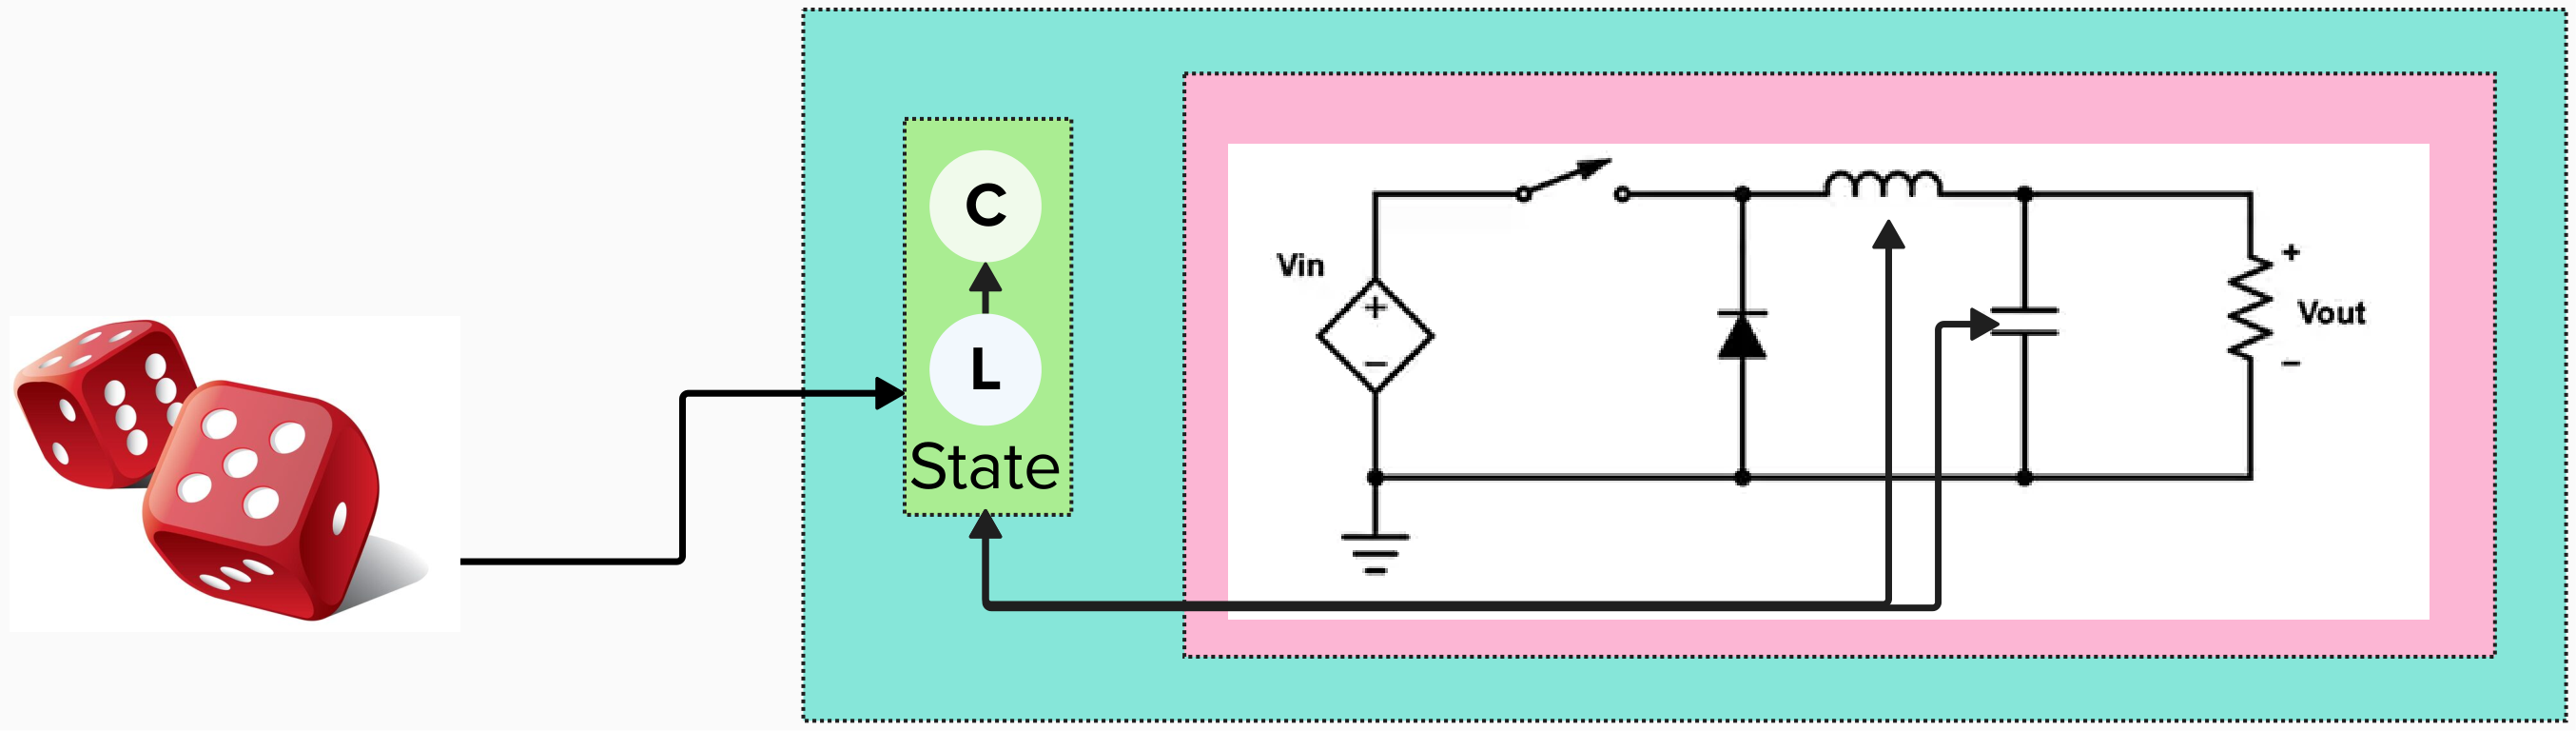
\includegraphics[width=0.7\textwidth]{3Experiment/2Experiment/1Random_Set_State.png}
\caption{Visualisierung der Zustandsgenerierung mit dem Würfel und die Setzung der Werte in der DCDC-Schaltung.}
\label{fig:state_generation}
\end{figure}

% \subsection{Makrozyklus Schritt 2: Entscheidungsfindung durch den Actor}

Nachdem der initiale Schaltungszustand durch eine Zufallsverteilung generiert wurde, kommt der Actor ins Spiel, der auf Basis der aktuellen Kapazitäts- (C) und Induktivitätswerte (L) Entscheidungen trifft. Der Actor, ein wesentlicher Bestandteil des Reinforcement Learning Systems, ist eine komplexe Funktion, die sich aus mehreren Gewichtungen (weights) und Verzerrungen (biases) zusammensetzt. Diese werden im Laufe des Vorwärtsdurchlaufs (Forward Propagation \ref{sec: Forward Propagation}) durch das Netzwerk multipliziert und summiert.

\begin{itemize}
		\item Innerhalb des Actors wird die Eingabe durch jede Schicht des neuronalen Netzwerks transformiert, wobei nach jedem Schichtdurchgang eine nicht-lineare Aktivierungsfunktion \ref{eq:activation_function} angewandt wird, um die Linearität der Operationen zu durchbrechen.
		\item Im spezifischen Kontext unseres Systems ist die Aktivierungsfunktion der letzten Schicht eine  Hyperbelfunktion (tanh), die die Ausgabe des Netzwerks beeinflusst und zu einem komplexen, nicht-linearen Ergebnis führt.
\end{itemize}

Die Ausgabe des Actors sind die PID-Werte, die für die Steuerung des nächsten Schrittes im System verwendet werden. Diese Werte sind das Resultat des durch die tanh-Funktion modifizierten Outputs und stellen somit eine fein abgestimmte Reaktion auf den Zustand der Schaltung dar. Diese Werte werden anschließend skaliert, um realistische PID-Reglerparameter zu erhalten:

\begin{itemize}
	\item Der Proportionalwert (Kp) wird zwischen 0 und 10 skaliert.
	\item Der Integralwert (Ki) wird zwischen 0 und 1 skaliert.
	\item Der Differentialwert (Kd) wird zwischen 0 und 0.1 skaliert.
\end{itemize}

Diese Skalierung ist entscheidend, um die Ausgangswerte des neuronalen Netzes in praktikable Steuerparameter zu überführen. Die Transformation gewährleistet, dass die PID-Werte in einem Bereich liegen, der für die Regelung des Systems adäquat ist und reflektiert die praktischen Anforderungen an die Systemsteuerung. 


\begin{figure}[htbp]
\centering
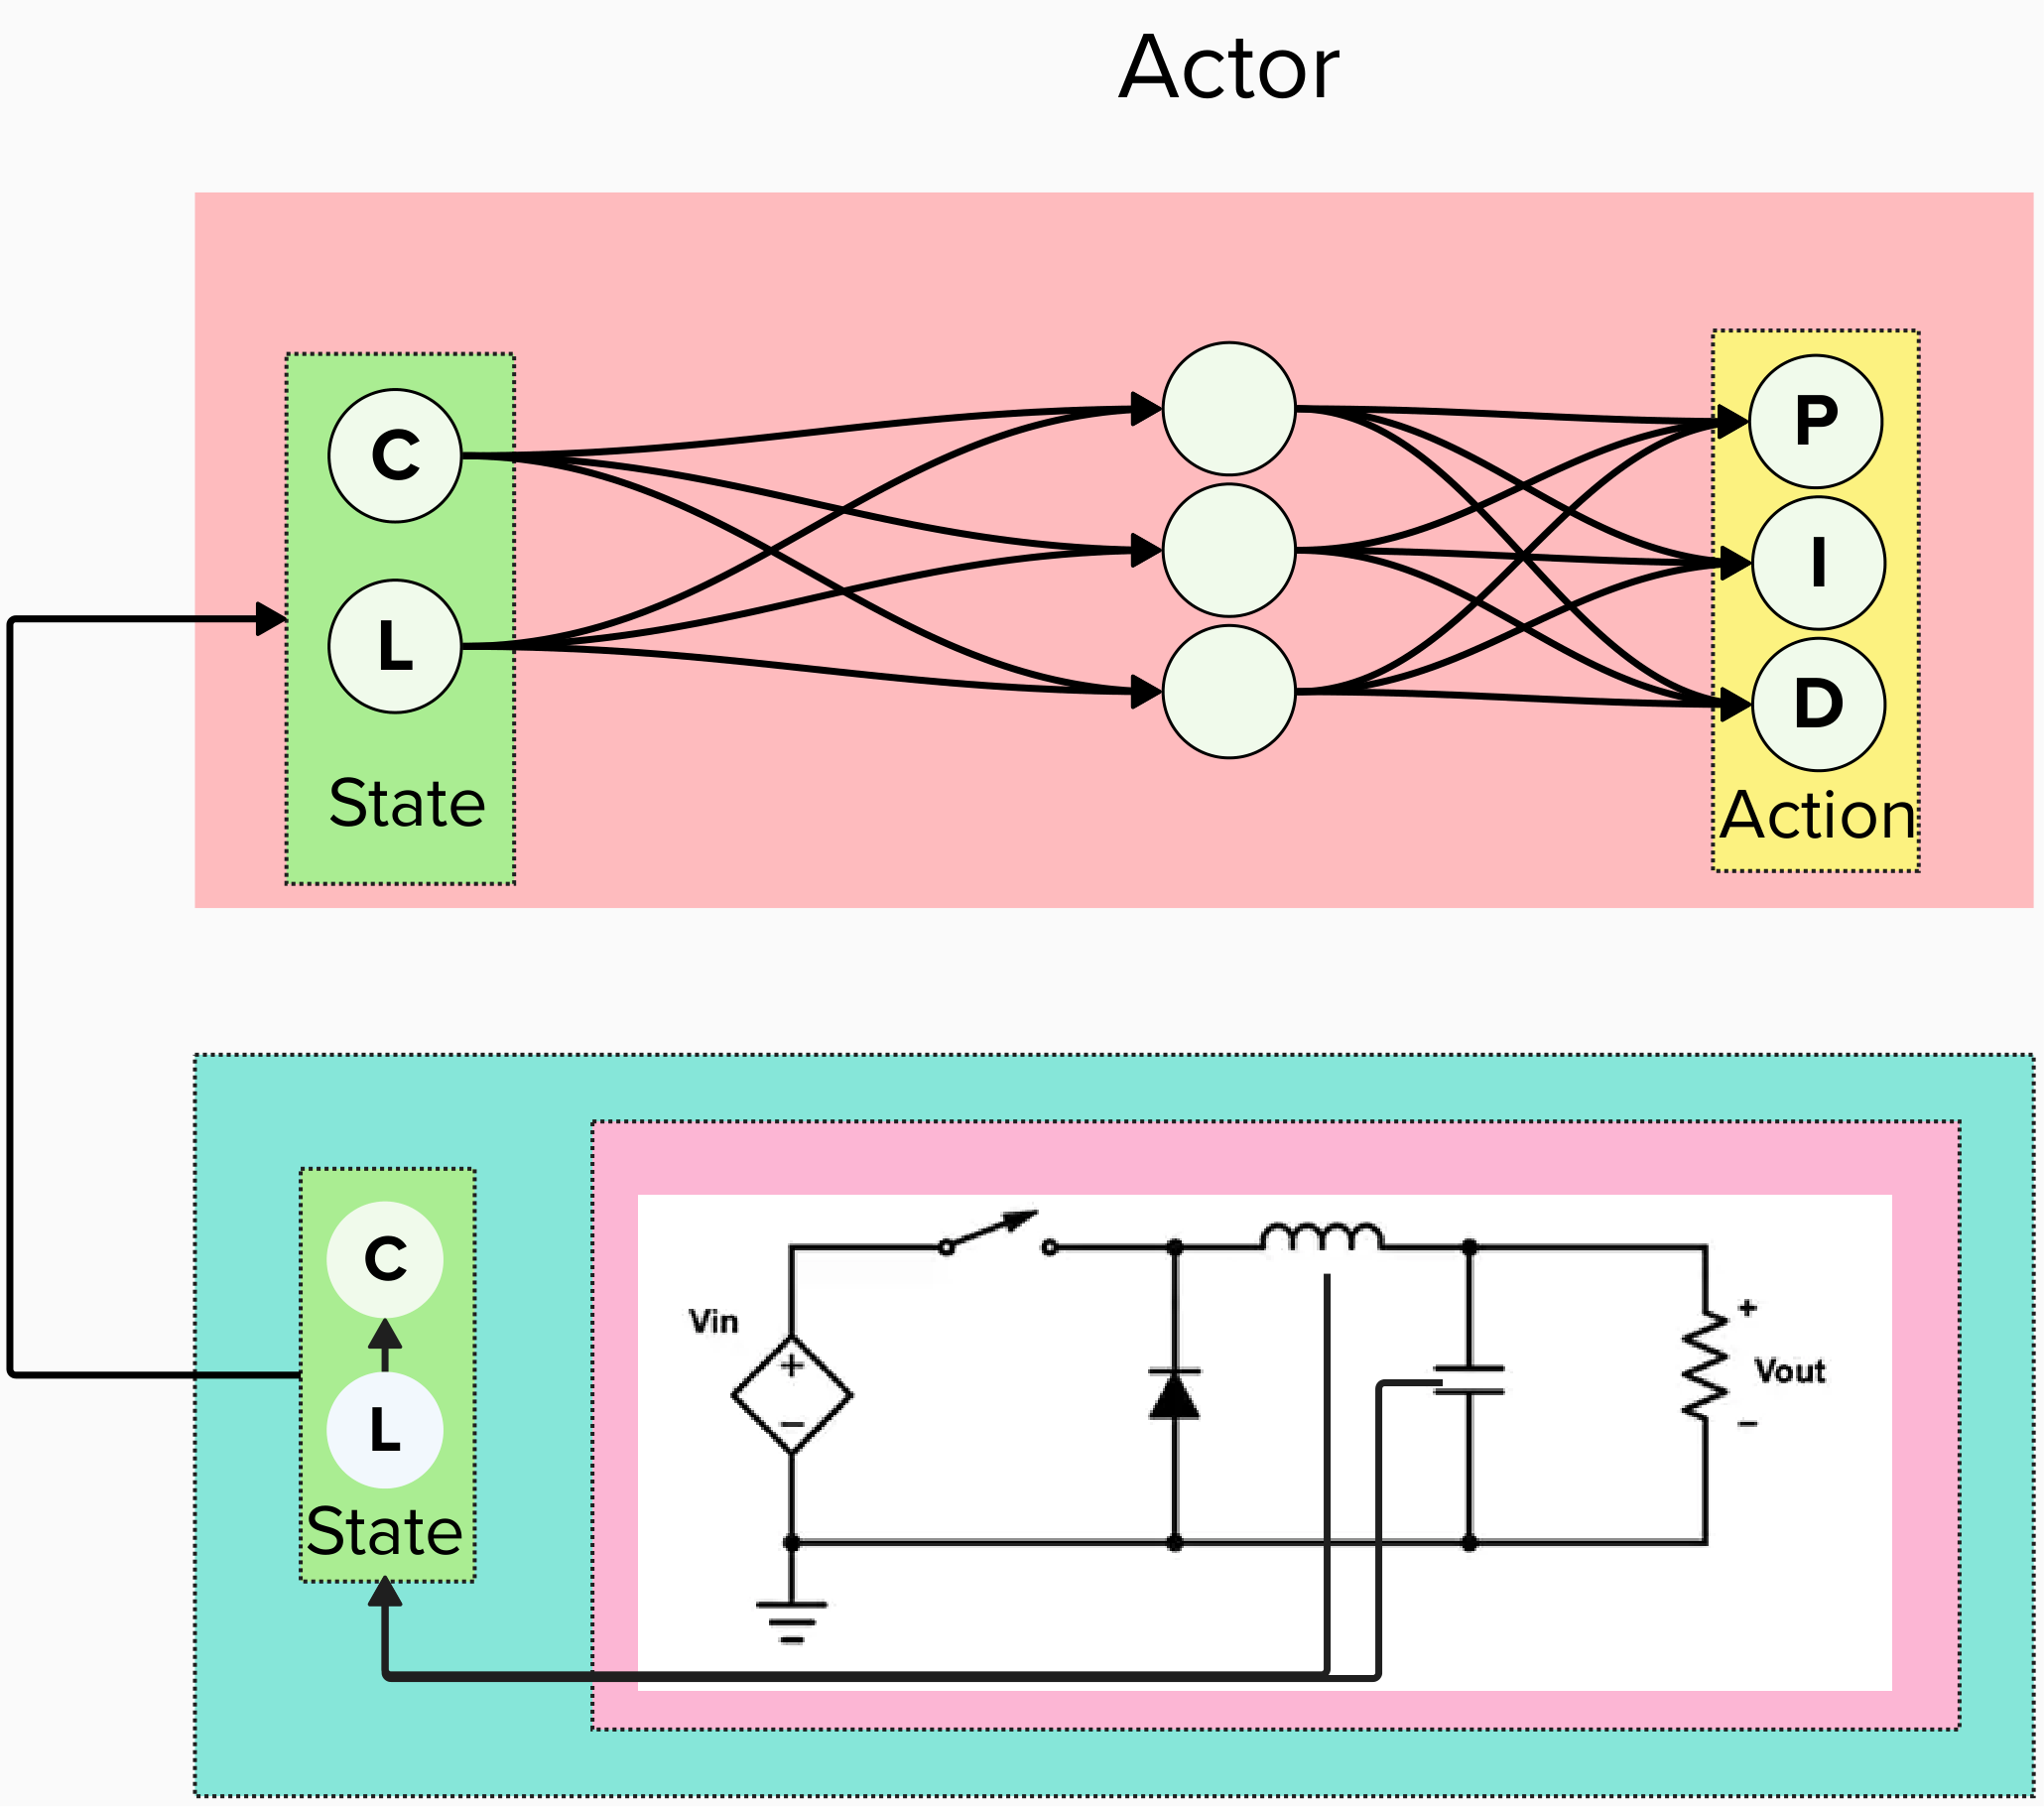
\includegraphics[width=0.5\textwidth]{3Experiment/2Experiment/2Actor.png}
\caption{Die Forward Propagation im Actor-Modul, die den Zustand S (C, L) aufnimmt und über ein mehrschichtiges neuronales Netzwerk PID-Aktionswerte ausgibt.}
\label{fig:actor_decision_making}
\end{figure}




\label{sec:Results_Presentation}

Nach der erfolgreichen  Realisierung einer robusten Actor-Critic-Architektur haben wir eine entscheidende Phase erreicht: die Präsentation unserer Forschungsergebnisse. Anfänglich zeigte unser Modell vielversprechende Resultate mit scheinbarer Leichtigkeit. Allerdings stellten wir fest, dass eine weitere Verfeinerung notwendig war, um exzellente Leistungswerte zu erzielen. Diese kontinuierliche Verbesserung war besonders im Feintuning-Prozess bemerkbar, wenngleich die Qualität der Ergebnisse anfangs unsicher war.

Um die Validität unserer Ergebnisse zu überprüfen, griffen wir auf Bayesian Optimization zurück, eine Technik, die für ihre herausragende Fähigkeit zur Auffindung optimaler Parameterwerte bekannt ist. Das Modell wurde speziell so konzipiert, dass es mit dieser Technik kompatibel ist.

Mit Bayesian Optimization konnten wir gezielt spezifischen Degradationszustand auswählen und diesen als Benchmark heranziehen. Diese gezielte Auswahl ermöglichte es uns, die Effektivität und Genauigkeit der Architektur zu bestätigen.

Abbildung \ref{fig:Bayesian_PID_Optimization} zeigt eine dreidimensionale Visualisierung verschiedener PID-Konfigurationen, die durch Bayesian Optimization ermittelt wurden. Die verschiedenen Farbnuancen korrespondieren mit den erzielten Rewards, wobei dunklere Farbtöne höhere Belohnungen symbolisieren. Die systematische und gleichmäßige Abtastung des Parameterraums durch Bayesian Optimization ist deutlich zu erkennen. Die Intensivierung der Suche in Bereichen, die vielversprechende Werte zeigten, verdeutlicht die zielgerichtete und effiziente Natur des Optimierungsprozesses.

\begin{figure}[h]
\centering
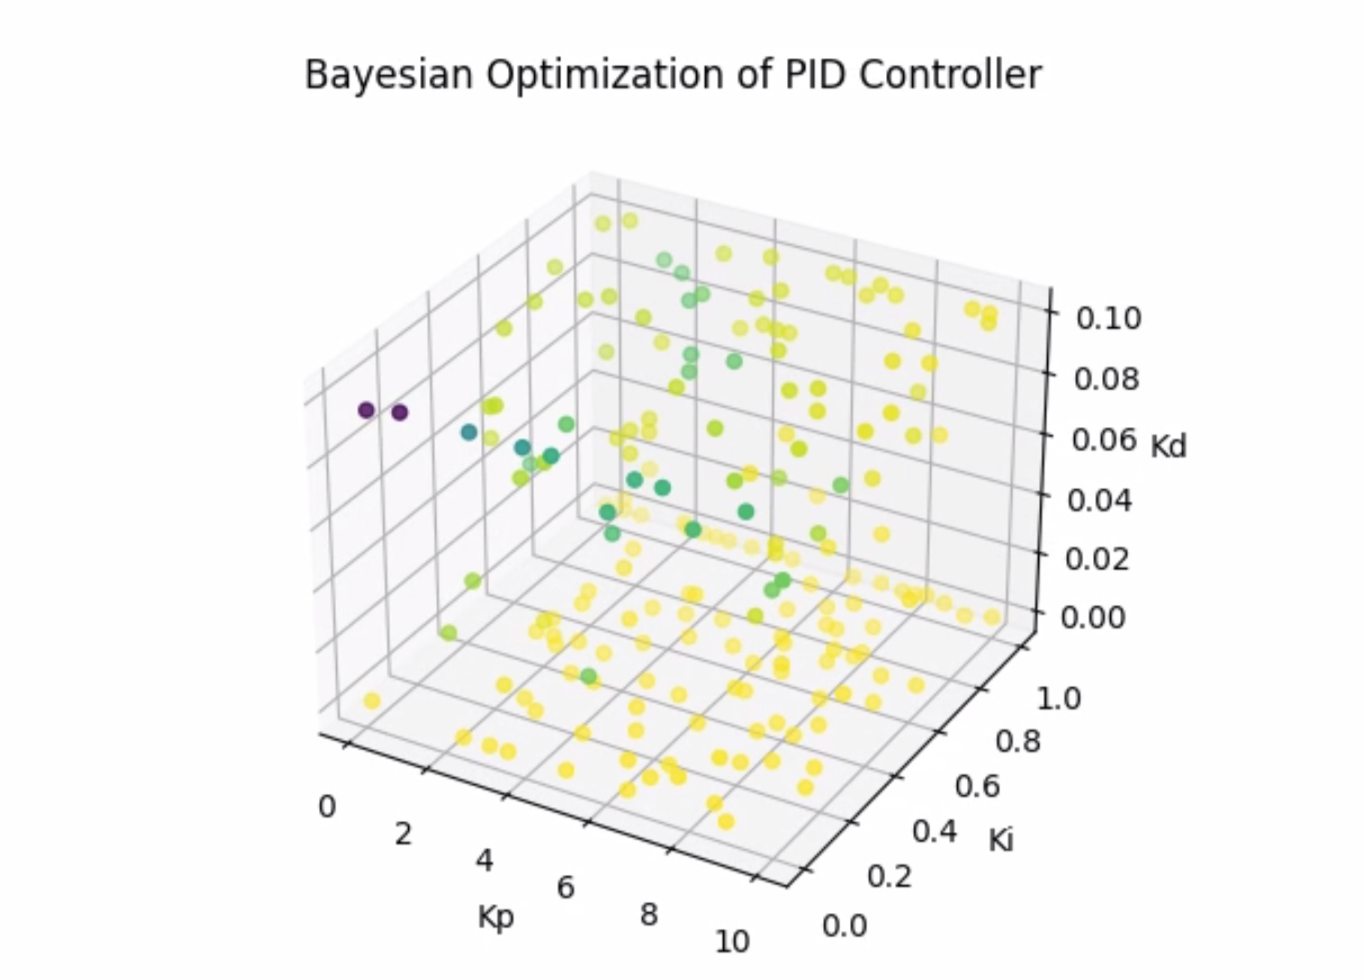
\includegraphics[width=0.6\textwidth]{4Ergebnisse/0Bayes_ergebnisse.png}
\caption{Dreidimensionale Darstellung der Bayesian Optimization von PID-Controller-Parametern.}
\label{fig:Bayesian_PID_Optimization}
\end{figure}

Die Präzision dieser Optimierungsmethode ermöglichte es uns, einen Referenzwert für die Regelungsleistung zu etablieren. Dieser Wert wurde anschließend als Benchmark für das manuelle Feintuning der Hyperparameter unserer Regelung verwendet.


\section{Hyperparameter}
\label{sec:Hyperparameter_Architecture_Comparison}
In diesem Abschnitt präsentieren wir eine Übersicht der Hyperparameter, unter denen unsere DDPG-Modelle trainiert wurden. Die Bedeutung dieser Parameter wurde bereits in einem früheren Kapitel detailliert erörtert. Hier fokussieren wir uns auf die spezifischen Einstellungen, die für das Training der unterschiedlichen Modelle verwendet wurden. 

\begin{table}[htbp]
		\centering
		\caption{Allgemeiner Vergleich der Hyperparameter für das kleine und große DDPG-Modell}
		\label{tab:hyperparameters_description}
		\begin{tabular}{lcc}
				\hline
				\textbf{Parameter} & \textbf{Einfaches Modell} & \textbf{Fortgeschrittenes Modell} \\				\hline
				ALPHA \ref{sec: Learnign Rate}  & Höhere Lernrate & Niedrigere Lernrate \\
				WORKER & Standardanzahl & Standardanzahl \\
				ITERATION & Einzeliteration & Einzeliteration \\
				STEPS & Weniger Trainingsschritte & Mehr Trainingsschritte \\
				BATCH\_SIZE \ref{sec: Batch} & Kleinere Batch-Größe & Größere Batch-Größe \\
				EXPLOITATION   & Standard-Exploitation & Standard-Exploitation \\
				LAYERS \ref{sec: Forward Propagation} & Weniger Schichten & Mehr Schichten \\
				LAYER\_1 & Standardanzahl Neuronen & Standardanzahl Neuronen \\
				LAYER\_2 & Standardanzahl Neuronen & Standardanzahl Neuronen \\
				NOISE \ref{sec: Exploration versus Exploitation}  & Moderate Exploration & Höhere Exploration \\
				GAMMA \ref{sec: discounted future reward}  & Keine Diskontierung & Keine Diskontierung \\
				\hline
		\end{tabular}
\end{table}

Die detaillierten Werte der Hyperparameter werden im folgenden Abschnitt präsentiert, wo wir spezifische Trainingsergebnisse und deren Vergleich darstellen. Die Auswahl und Einstellung dieser Parameter spielen eine entscheidende Rolle im Lernprozess der Modelle und beeinflussen maßgeblich deren Leistung und Effizienz. Im folgenden Abschnitt werden wir die spezifischen Trainingsresultate und ihre Validierung detailliert präsentieren.

\section{Methodik des Vergleichs}
Zur Validierung der Leistung unserer Modelle haben wir uns für eine spezifische Herangehensweise entschieden, die sich von der Standardtrainingsroutine unterscheidet. Anstatt das Modell kontinuierlich durch den gesamten Trainingspool lernen zu lassen, wurde jeder zehnte "EXPLOITATION" Schritt genutzt, um das Modell anhand eines vordefinierten Referenzwertes zu evaluieren. Dieser Referenzwert wurde bewusst nicht in das Training einbezogen, um eine unabhängige Beurteilung der Modellleistung zu ermöglichen. Die deterministische Natur unserer Netzwerke erleichterte diesen Prozess erheblich, da sie nach dem Training konsistente und wiederholbare Ergebnisse liefern. Dies ermöglichte es uns, die Leistung des Modells präzise zu beurteilen, ohne dass eine Mittelung über mehrere Zustände erforderlich war, wie es bei stochastischen Modellen der Fall gewesen wäre. Die deterministische Architektur gewährleistet, dass die gleichen Eingaben stets zu denselben Ausgaben führen, was die Validierung und das Testen vereinfacht und zuverlässiger macht.

% \section{Detaillierte Darstellung und Vergleich der Ergebnisse}
\label{sec:Detailed_Results_Comparison}

In diesem Abschnitt werden die Ergebnisse der drei verschiedenen Ansätze zur Optimierung des DC-DC-Wandlers vorgestellt: die Bayesianische Optimierung sowie die kleinen und großen DDPG-Netzwerkmodelle. Die Belohnungen, die mit jeder Konfiguration erzielt wurden, bieten einen Einblick in die Effektivität jedes Ansatzes.




\begin{table}[htbp]
\centering
\caption{Vergleich der erzielten Belohnungen der Optimierungsansätze}
\label{tab:rewards_comparison}
\begin{tabular}{lcc}
\hline
\textbf{Ansatz} & \textbf{Belohnung} & \textbf{Konfiguration} \\
\hline
Bayesian Optimization & -3.63 & - \\
Kleines DDPG-Modell & -3.9098342748323116 & \begin{tabular}[c]{@{}c@{}}Induktivität: 5.0e-3, \\ Kapazität: 10.0e-6, \\ Kp: 2.43055224, \\ Ki: 0.67658715, \\ Kd: 0.00937204\end{tabular} \\
Großes DDPG-Modell & -3.42173412748323116 & \begin{tabular}[c]{@{}c@{}}Induktivität: 5.0e-3, \\ Kapazität: 10.0e-6, \\ Kp: 3.42173412, \\ Ki: 0.67770964, \\ Kd: 0.01268652\end{tabular} \\
\hline
\end{tabular}
\end{table}

Jeder Ansatz wurde unter Verwendung einer spezifischen Kombination von Induktivität und Kapazität evaluiert, wobei die entsprechenden Belohnungen als Maßstab für die Leistungsfähigkeit dienten.

% Wiederholen Sie die obige Struktur für die anderen beiden Ansätze.

Die erzielten Belohnungen sind in den entsprechenden Grafiken visualisiert, welche die Leistung jedes Modells über die Zeit darstellen. Diese Visualisierungen sind entscheidend, um die Fortschritte und das Verhalten des DC-DC-Wandlers in Echtzeit zu verstehen.


\clearpage % Dies sorgt dafür, dass die folgenden Inhalte auf einer neuen Seite beginnen.

Die Abbildungen \ref{fig:bayesian_optimization_results}, \ref{fig:small_ddpg_results} und \ref{fig:large_ddpg_results} zeigen die jeweiligen Belohnungen, die durch die unterschiedlichen Optimierungsverfahren erzielt wurden. Die Belohnungen reflektieren die Anpassungsfähigkeit und Effizienz der jeweiligen Regelungsmethoden unter verschiedenen Bedingungen.

\subsection{Analyse der Ergebnisse}
Die direkte Gegenüberstellung der Belohnungen aus den verschiedenen Optimierungsansätzen zeigt deutlich, dass das größere DDPG-Modell eine überlegene Performance aufweist, insbesondere in der Anpassungsfähigkeit an komplexe Regelungsaufgaben. Die Bayesianische Optimierung liefert eine gute Grundlage für das Feintuning, während das kleinere DDPG-Modell trotz geringerer Komplexität wettbewerbsfähige Ergebnisse zeigt.

Diese vergleichende Analyse ermöglicht es uns, die Vor- und Nachteile jedes Ansatzes zu verstehen und bietet wertvolle Einblicke für die zukünftige Entwicklung von Regelungsalgorithmen für elektronische Wandler.










% 12 Ergebnisee Bestrafe Spikes

Baysie Optimization
Maximum Value: -3.821364055276552
Corresponding Parameters:
Kd: 0.013931402806247174
Ki: 0.8521257369717544
Kp: 3.925047356012834


Netzwerk Small:
Maximum reward: -3.910180285904306
Corresponding action: 5.32709267 0.99218339 0.01846072
File containing maximum reward: unique_name_Artemis_2023-1

Ergebnise das big network 
Maximum reward: -3.7855736817205585
Corresponding action: 5.03869285 0.80699286 0.01712556



\section{Vergleich und Validierung der Modellleistung}


Im Folgenden wird der umfassende Lernprozess des DDPG-Modells dargestellt, wobei ein besonderes Augenmerk auf die ersten 10.000 Iterationen gelegt wird, wie in Abbildung \ref{fig:ddpg-learning-phases} zu sehen ist. Dieser Abschnitt des Trainings ist besonders aussagekräftig, da abgesehen von den divergierenden Modellen, alle anderen Modelle nahe am Optimum zu konvergieren scheinen.


\paragraph{Phase 1: Verifikation und Robustheit des DDPG-Modells}
Die erste Phase unserer Untersuchung dient der Verifikation der Leistungsfähigkeit und Robustheit des Deep Deterministic Policy Gradient (DDPG)-Modells im Kontext der Optimierung von DC-DC-Wandlern. Hierbei konzentrieren wir uns auf zwei Varianten des DDPG-Modells: ein einfacheres, schnell zu trainierendes Modell und ein fortgeschrittenes Modell mit komplexerer Architektur und längeren Trainingszeiten. Unser Hauptziel ist es, zu demonstrieren, dass das DDPG-Modell in der Lage ist, nahezu optimale Lösungen zu erzielen.

Um die Gültigkeit und Zuverlässigkeit unserer Modelle zu bestätigen, vergleichen wir die Ergebnisse des DDPG-Modells mit denen eines anderen bekannten Optimierungsverfahrens, das für seine hohe Leistung bekannt ist. Diese methodische Triangulation – die Approximation der Lösungen durch zwei grundlegend verschiedene Ansätze – soll nicht nur die Ähnlichkeit der Ergebnisse aufzeigen, sondern auch die Stärke und Anpassungsfähigkeit des DDPG-Modells in diesem speziellen Anwendungsbereich unterstreichen. Wir analysieren, wie sich eine einfache quadratische Belohnungsfunktion, die die Abweichung von der Zielspannung bestraft, auf die Performance dieser Modelle auswirkt und wie dies im Vergleich zu dem alternativen Optimierungsverfahren steht.

\paragraph{Phase 2: Anpassung der Bestrafungsfunktion und Erweiterung des Suchraums}
In der zweiten Phase unserer Untersuchung wurde die Belohnungsfunktion modifiziert, um eine ausgewogenere Reaktion auf Spannungsabweichungen zu erzielen. Wir haben zwei Ansätze kombiniert: Für Spannungsabweichungen über einem Schwellenwert von 1 wird eine quadratische Bestrafung angewendet, um auf größere Spannungsschwankungen stärker zu reagieren und so die Stabilität des Systems zu verbessern. Für Abweichungen unter diesem Schwellenwert wird eine Bestrafung basierend auf dem absoluten Wert vorgenommen, was das System sensibler für kleinere Spannungsabweichungen macht.

Zusätzlich wurde der Suchraum für die Optimierung erheblich erweitert, um eine breitere Palette von Konfigurationsmöglichkeiten zu erforschen. Der neue Suchraum erstreckt sich nun über deutlich größere Bereiche:
- Kp: 0 bis 1000
- Ki: 0 bis 100
- Kd: 0 bis 10

Diese Erweiterung des Suchraums soll aufzeigen, wie sich die Modelle, insbesondere die Bayesianische Optimierung, die bei großen Suchräumen bekannterweise Herausforderungen hat, im Vergleich zum DDPG-Modell verhalten. Es wird interessant zu beobachten sein, wie diese Änderungen die Leistung und Effektivität der Modelle beeinflussen, insbesondere in Bezug auf ihre Fähigkeit, mit größeren und komplexeren Konfigurationsräumen umzugehen.

\paragraph{Phase 3: Miniaturisierung}

In der dritten Phase unserer Untersuchung widmen wir uns der Miniaturisierung der Netzwerkmodelle. Unser Ziel ist es, die Fähigkeiten eines reduzierten Modells zu evaluieren und zu verstehen, wie es trotz geringerer Komplexität effektiv funktionieren kann. Diese Untersuchungen sind entscheidend, um das Potenzial der kompakten Modelle für den Einsatz in realen Anwendungsszenarien zu erkennen.

% \textbf{Erwartete Auswirkungen:}
% Durch diese Anpassung erwarten wir, dass die Modelle eine feinere Abstimmung der Spannungsregelung erlernen und gleichzeitig eine robustere Reaktion auf größere Spannungsschwankungen zeigen. Dieser Ansatz soll die Balance zwischen Sensitivität für geringfügige Abweichungen und effektiver Kontrolle über größere Störungen verbessern.


\section{Phase 1: Einfache und Fortgeschrittene Netzwerkmodelle}
\label{subsec:Basic_Advanced_Models}

In diesem Abschnitt werden die Ergebnisse der drei verschiedenen Ansätze zur Optimierung des DC-DC-Wandlers vorgestellt: die Bayesianische Optimierung sowie die kleinen und großen DDPG-Netzwerkmodelle. Die Belohnungen, die mit jeder Konfiguration erzielt wurden, bieten einen Einblick in die Effektivität jedes Ansatzes.

\paragraph{Hyperparameter}

\begin{table}[htbp]
\centering
\caption{Erweiterter Vergleich der Hyperparameter für das kleine und große DDPG-Modell unter Einbeziehung des Parameterraums}
\label{tab:extended_hyperparameters}
\begin{tabular}{lcc}
\hline
\textbf{Parameter} & \textbf{Kleines Modell} & \textbf{Großes Modell} \\
\hline
ALPHA & 0.001 & 0.0001 \\
WORKER & 12 & 12 \\
ITERATION & 1 & 1 \\
STEPS & 2000 & 20000 \\
BATCH\_SIZE & 72 & 250 \\
EXPLOITATION & 10 & 10 \\
LAYERS & 2 & 12 \\
LAYER\_1 & 158 & 158 \\
LAYER\_2 & 52 & 52 \\
NOISE & 0.3 & 0.45 \\
GAMMA & 0.0 & 0.0 \\
\textbf{Kp-Bereich} & 0 bis 10 & 0 bis 10 \\
\textbf{Ki-Bereich} & 0.0 bis 1.0 & 0.0 bis 1.0 \\
\textbf{Kd-Bereich} & 0.0 bis 0.2 & 0.0 bis 0.2 \\
\hline
\end{tabular}
\end{table}

\begin{figure}[htbp]
\centering
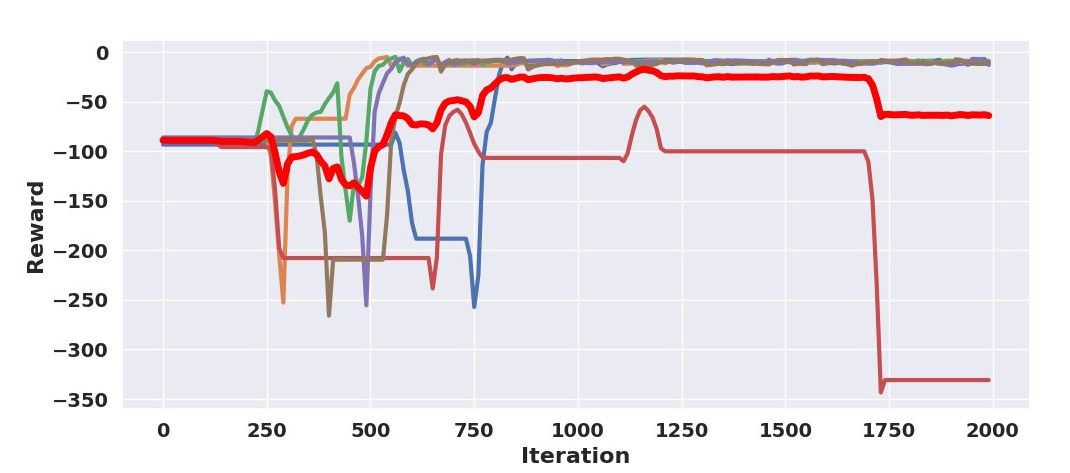
\includegraphics[width=0.7\textwidth]{4Ergebnisse/Phasen/1Phase/1Q_klein_epoch.png}
\caption{Belohnungsentwicklung über die Zeit für das kleine DDPG-Modell.}
\end{figure}

\begin{figure}[htbp]
\centering
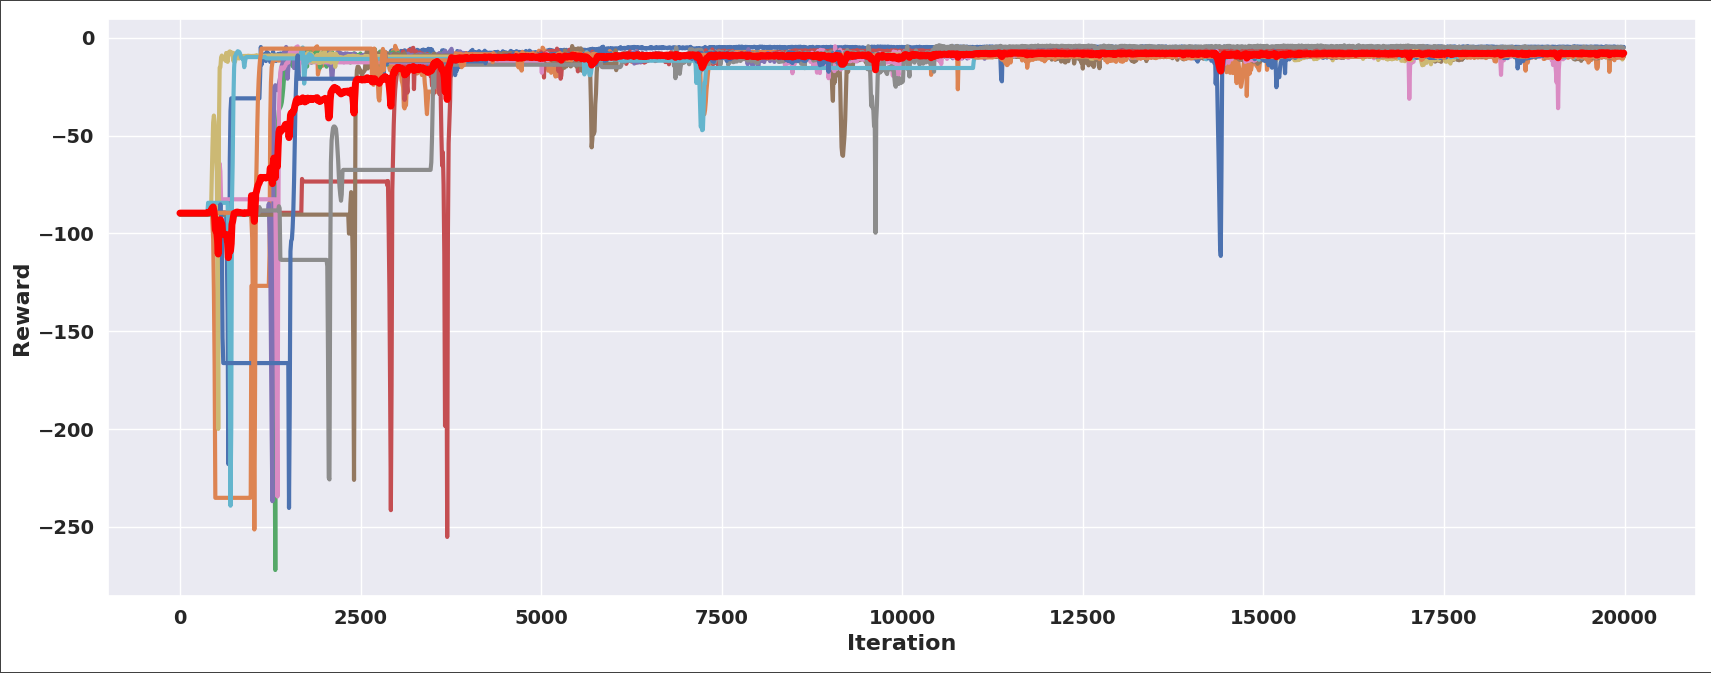
\includegraphics[width=0.92\textwidth,  trim=10px 10px 10px 10px, clip]{4Ergebnisse/Phasen/1Phase//1R_gross_epoch.png}
\caption{Belohnungsentwicklung über die Zeit für das große DDPG-Modell.}
\end{figure}


\begin{table}[htbp]
\centering
\caption{Vergleich der Ergebnisse verschiedener Modelle}
\label{tab:model_comparison}
\begin{tabular}{|c|c|c|}
\hline
\textbf{Modell} & \textbf{Ergebnis} & \textbf{Parameter} \\
\hline
Bayesian Optimization & -3.63 & 
\begin{tabular}[c]{@{}c@{}}Induktivität: 5.0e-3\\ Kapazität: 10.0e-6\\ Kp: 3.9250\\ Ki: 0.8521\\ Kd: 0.0139\end{tabular} \\
\hline
Kleines DDPG-Modell & -3.9098 & 
\begin{tabular}[c]{@{}c@{}}Induktivität: 5.0e-3\\ Kapazität: 10.0e-6\\ Kp: 2.4306\\ Ki: 0.6766\\ Kd: 0.0094\end{tabular} \\
\hline
Großes DDPG-Modell & -3.4217 & 
\begin{tabular}[c]{@{}c@{}}Induktivität: 5.0e-3\\ Kapazität: 10.0e-6\\ Kp: 3.4217\\ Ki: 0.6777\\ Kd: 0.0127\end{tabular} \\
\hline
\end{tabular}
\end{table}


\begin{figure}[htbp]
\centering
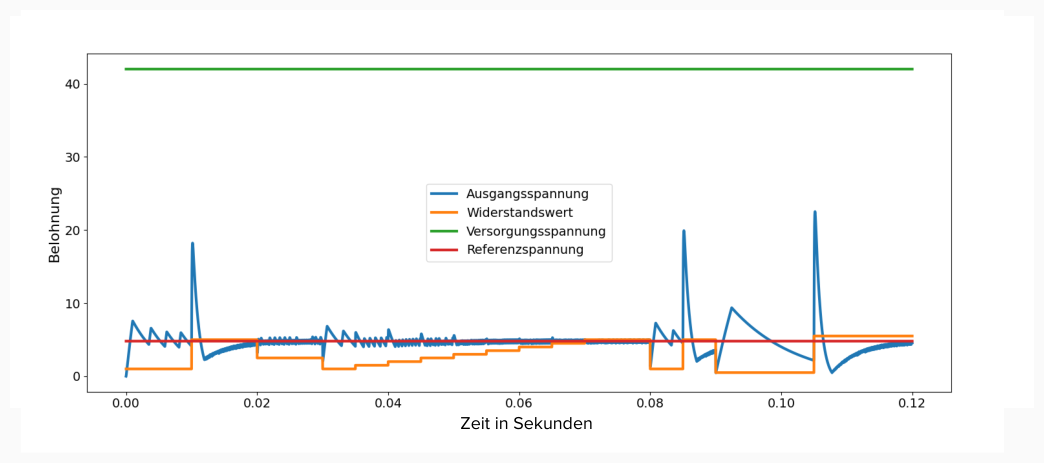
\includegraphics[width=0.99\textwidth, trim=10px 10px 10px 10px, clip]{4Ergebnisse/Phasen/1Phase/1S_small_search_space_bayes.png}
\caption{Darstellung des Regelungsverhaltens eines durch Bayes'sche Optimierung eingestellten PID-gesteuerten DC-DC-Konverters. Die Grafik zeigt die Belohnungsentwicklung über die Zeit und reflektiert die Anpassung der Ausgangsspannung (blau) an die Referenzspannung (rot) unter Berücksichtigung der Versorgungsspannung (grün) und des Widerstandswertes (orange). Die Ergebnisse verdeutlichen die Effektivität der Bayes'schen Optimierung bei der Feinabstimmung des Reglers für eine stabile Spannungsregelung.}
\label{fig:bayesian_optimization_pid_control}
\end{figure}
%
\begin{figure}[htbp]
\centering
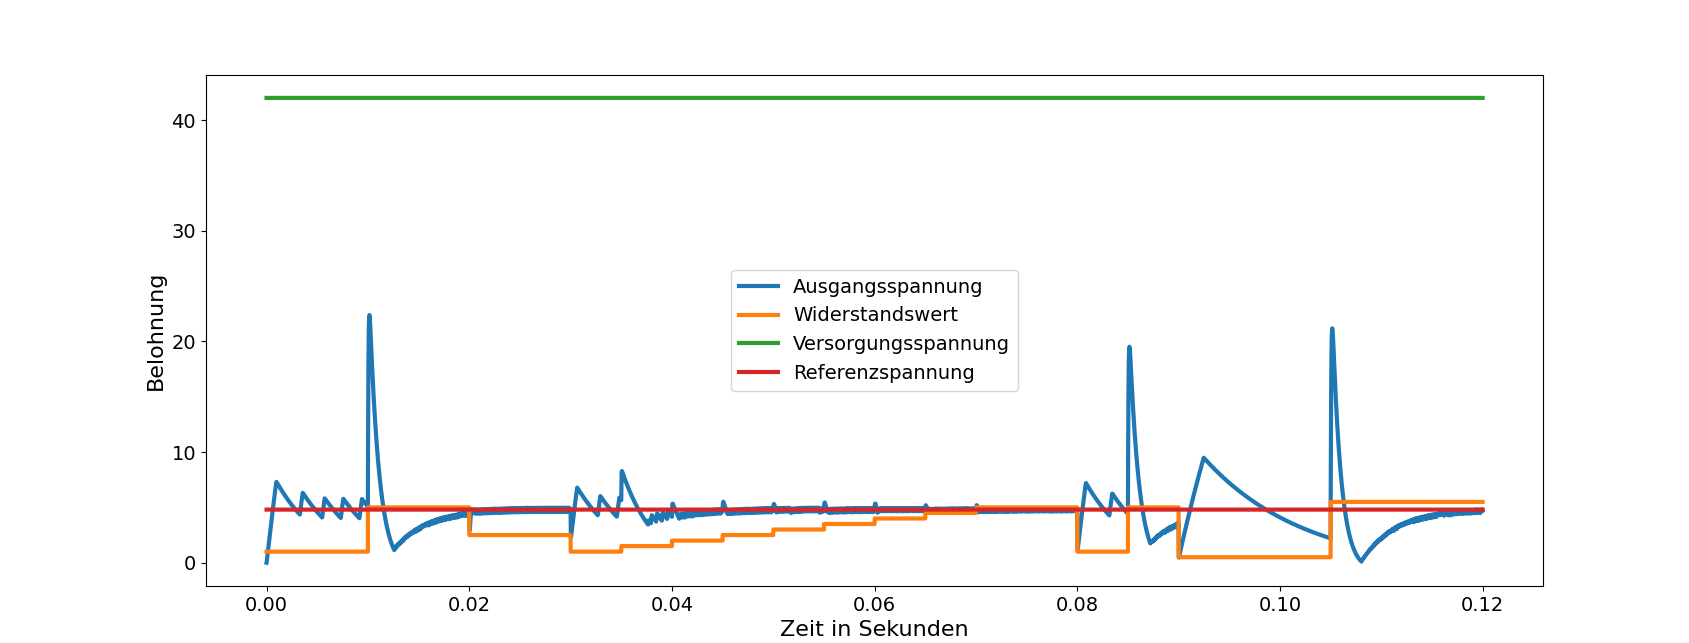
\includegraphics[width=0.99\textwidth]{4Ergebnisse/Phasen/1Phase//1T_small_search_space_small_net_dcdc.png}
\caption{Regelungsverhaltens über die Zeit für das kleine DDPG-Modell.}
\label{fig:small_ddpg_results}
\end{figure}
%
\begin{figure}[htbp]
\centering
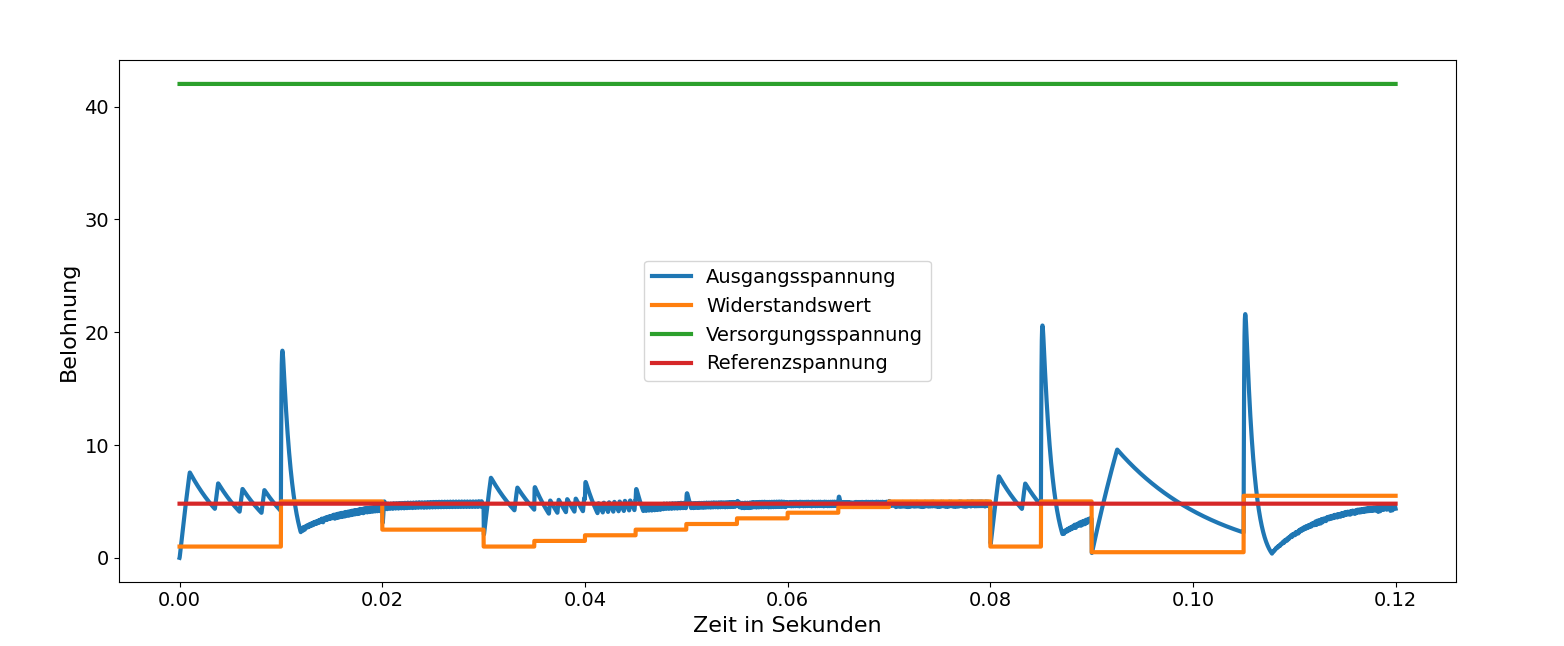
\includegraphics[width=0.99\textwidth]{4Ergebnisse/Phasen/1Phase//1U_big_net_dcdc.png}
\caption{Regelungsverhaltens über die Zeit für das große DDPG-Modell.}
\label{fig:large_ddpg_results}
\end{figure}

Die Abbildungen \ref{fig:bayesian_optimization_results}, \ref{fig:small_ddpg_results} und \ref{fig:large_ddpg_results} zeigen die jeweiligen Belohnungen, die durch die unterschiedlichen Optimierungsverfahren erzielt wurden.

\paragraph{Analyse der Ergebnisse: Leistungsvergleich der Optimierungsansätze}
Bei der Betrachtung der erzielten Ergebnisse aus den verschiedenen Optimierungsansätzen wird deutlich, dass sich die Leistungsdifferenzen vor allem im Belohnungswert (Reward) widerspiegeln. Alle drei Ansätze - Bayesianische Optimierung, kleines und großes DDPG-Modell - waren in der Lage, eine optimale oder nahezu optimale Lösung für die gestellte Aufgabe zu finden, wobei die Unterschiede in den tatsächlichen Spannungsverläufen minimal waren.

Interessanterweise zeigte das kleinere DDPG-Modell die geringste Leistung, was sich sowohl in niedrigeren Belohnungswerten als auch in einer weniger stabilen Konvergenz äußerte. Im Gegensatz dazu erreichte das große DDPG-Modell die besten Belohnungswerte, wobei alle Modelle eine gewisse Leichtigkeit bei der Konvergenz zeigten. Die Bayesianische Optimierung lag in ihrer Leistung dazwischen.

\paragraph{Synthese der Ergebnisse}

Interessanterweise zeigen sowohl die Bayesianische Optimierung als auch die DDPG-Modelle in ihren jeweiligen Anwendungen bemerkenswerte Übereinstimmungen in ihren Ergebnissen. Diese Konsistenz unterstreicht die Robustheit unserer Methoden und die Verlässlichkeit der erzielten Optimierungen. Trotz der unterschiedlichen Herangehensweisen und Techniken, die bei diesen beiden Methoden zum Einsatz kommen, konvergieren ihre Ergebnisse hin zu ähnlichen Lösungen. Dies deutet darauf hin, dass beide Ansätze effektiv die kritischen Bereiche des Parameterraums identifizieren und optimieren, was ein zentrales Ziel unserer Forschung ist.


\section{Phase 2: Vertiefte Analyse und Optimierung in Erweiterten Parameterräumen}
\label{subsec:Detailed_Learning_Process_Phase2}


\input{4Ergebnisse/Phasen/2Phase/2Phase_Einleitung.tex}

\begin{figure}[htbp]
\centering
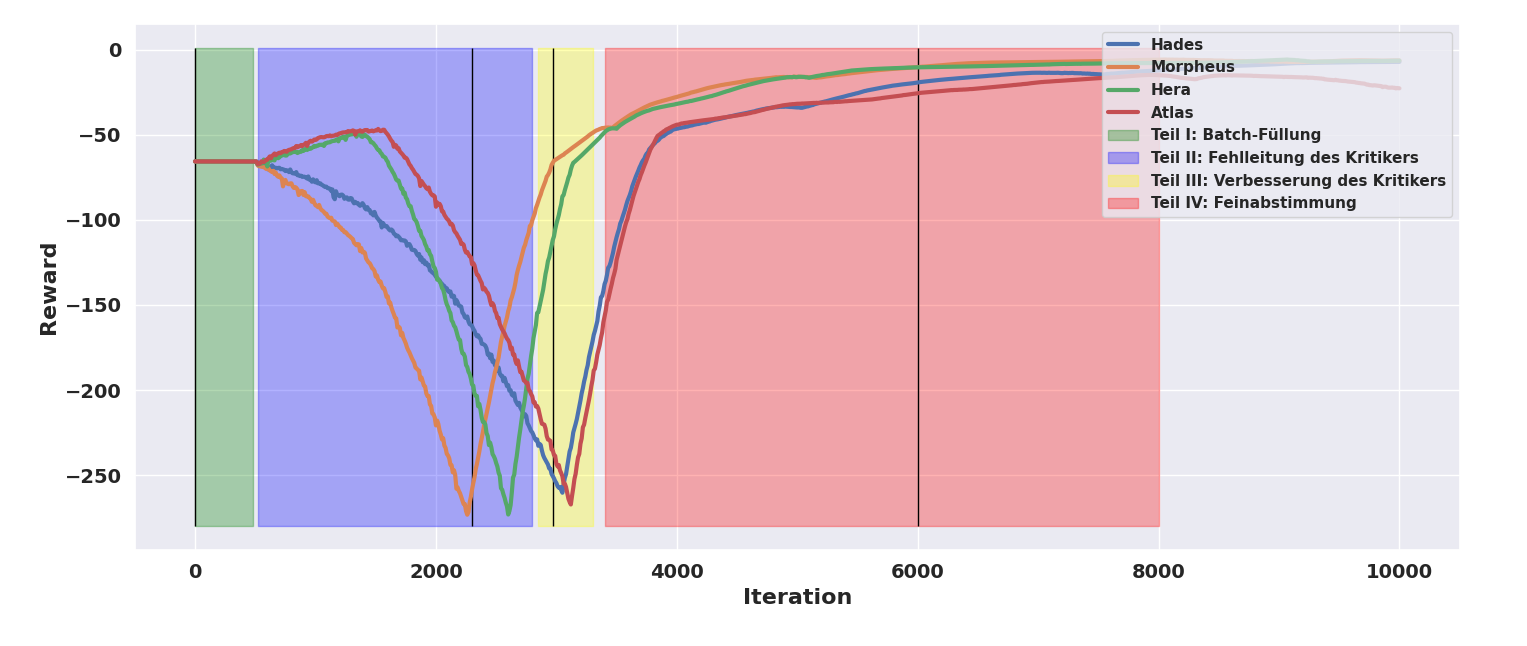
\includegraphics[width=\textwidth]{4Ergebnisse/Phasen/2Phase/4_0Presentation_of_Phase.png.png}
\caption{Detaillierte Darstellung der Lernprozesse und ausgewählten Stichproben in den verschiedenen Phasen des DDPG-Modells.}
\label{fig:ddpg-learning-phases}
\end{figure}

 Die initiale Selektion für die detaillierte Analyse fokussiert auf die Modelle, die zu Beginn des Trainings die besten Resultate aufweisen. Diese Vorauswahl basiert auf der Performance und der Konvergenzgeschwindigkeit in den ersten 10.000 Iterationen, wie Abbildung \ref{fig:ddpg-learning-phases} illustriert. Diese Modelle zeigen eine effektive Anpassung an den erweiterten Parameterraum und lassen auf ein optimiertes Lernverhalten schließen.


\input{4Ergebnisse/Phasen/2Phase/TeilI.tex}
\input{4Ergebnisse/Phasen/2Phase/TeilII.tex}
\input{4Ergebnisse/Phasen/2Phase/TeilIII.tex}
\input{4Ergebnisse/Phasen/2Phase/TeilIV.tex}
\input{4Ergebnisse/Phasen/2Phase/TeilV.tex}
\input{4Ergebnisse/Phasen/2Phase/z_Synthese.tex}

\section{Phase 3: Miniaturisierung und Leistungsanalyse}
\label{subsec:Network_Miniaturization_Performance_Analysis}


\begin{table}[htbp]
\centering
\caption{Konfiguration und Ergebnisse des miniaturisierten Modells}
\label{tab:miniaturization_results}
\begin{tabular}{lc}
\hline
\textbf{Parameter} & \textbf{Wert} \\
\hline
ALPHA & \( 1 \times 10^{-5} \) \\
WORKER & 10 \\
ITERATION & 1 \\
STEPS & 30000 \\
BATCH\_SIZE & 250 \\
EXPLOITATION & 10 \\
LAYERS & 3 \\
LAYER\_1 & 10 \\
LAYER\_2 & 3 \\
NOISE & 0.4 \\
GAMMA & 0.0 \\
\hline
Maximale Belohnung & -4.29 \\
Entsprechende Aktion & [6.84119821, 0.75633377, 0.02226542] \\
\hline
\end{tabular}
\end{table}

Die Ergebnisse der Miniaturisierung sind bemerkenswert, da das verkleinerte Modell eine maximale Belohnung von -4.295256034278478 erreichte, was auf eine nahezu optimale Regelungsleistung hindeutet. Die entsprechenden Aktionen und detaillierten Konfigurationen des Modells sind in Tabelle \ref{tab:miniaturization_results} aufgeführt.

\begin{figure}[htbp]
\centering
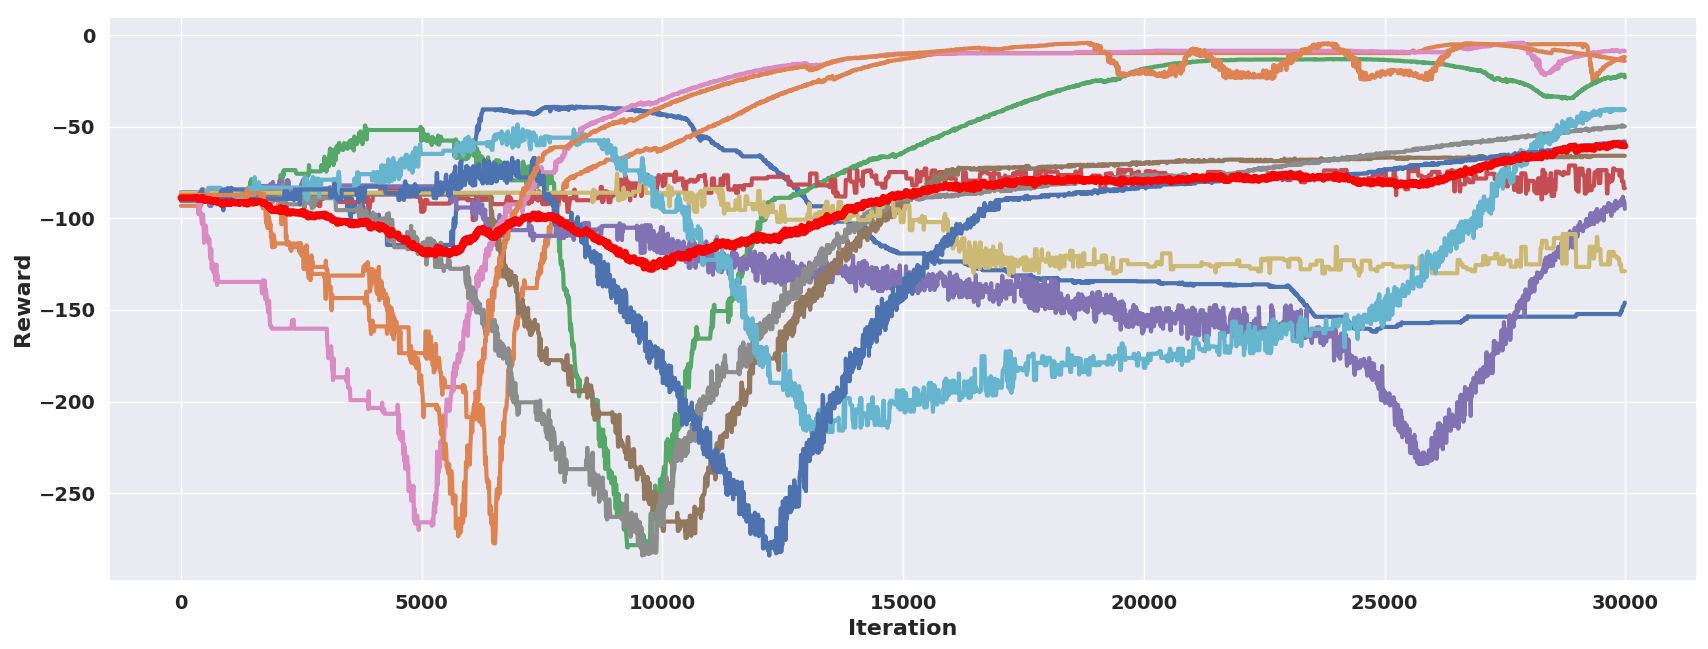
\includegraphics[width=\textwidth]{4Ergebnisse/Phasen/3Phase/3R_big_training_minimize_epoch.png}
\caption{Leistungskurve des miniaturisierten Modells über die Trainingsdauer.}
\label{fig:miniaturized_model_performance}
\end{figure}

Die Leistung des miniaturisierten Modells, wie in Abbildung \ref{fig:miniaturized_model_performance} gezeigt, demonstriert eindrucksvoll, dass eine effiziente Modellminiaturisierung ohne erheblichen Leistungsverlust möglich ist. Diese Erkenntnis ist besonders relevant für praxisnahe Anwendungen, wo kompakte Modelle aufgrund von 
Ressocenbe- schränkungen bevorzugt werden.

Die Ergebnisse wurden durch eine Kombination aus niedriger Lernrate und einer hohen Anzahl von Trainingsepochen erzielt. Die erzielten Ergebnisse \ref{fig:miniaturized_model_performance} weisen darauf hin, dass das Modell trotz der frühzeitigen Beendigung des Trainings bereits eine beachtliche Leistung demonstrierte. Dies legt nahe, dass mit einer Fortsetzung des Trainingsprozesses und einer weiteren Feinabstimmung der Hyperparameter möglicherweise noch höhere Performanzwerte hätten erreicht werden können. Die vorliegenden Ergebnisse bestätigen somit nicht nur die Effektivität des eingesetzten Trainingsansatzes, sondern auch das Potenzial für weitergehende Verbesserungen und Optimierungen.

Ein weiterer wichtiger Aspekt ist das Risiko des Overfittings bei komplexeren Modellen, wie bereits in Kapitel \ref{sec: overfitting} diskutiert. Overfitting tritt auf, wenn ein Modell zu sehr auf die spezifischen Trainingsdaten ausgerichtet ist und dadurch seine Fähigkeit verliert, auf neue, unbekannte Daten angemessen zu reagieren. Es ist eine bekannte Tatsache, dass einfachere Modelle häufig eine bessere Generalisierungsfähigkeit aufweisen, da sie weniger anfällig für das Auswendiglernen spezifischer Trainingsdaten sind. Unsere Ergebnisse zeigen, dass das miniaturisierte Modell trotz seiner Einfachheit eine gute Leistung erbringen konnte, was die Wichtigkeit einer ausgewogenen Modellkomplexität in der Modellentwicklung hervorhebt. 

Insgesamt legen diese Beobachtungen nahe, dass es vorteilhaft sein kann, sich auf die Optimierung von Hyperparametern zu konzentrieren, um kleinere, aber leistungsfähige Modelle zu entwickeln.



% \input{4Ergebnisse/9Disskusion}


\chapter{Diskussion}
\label{sec:Discussion}

In dieser Studie wurde der Deep Deterministic Policy Gradient (DDPG) Algorithmus zur Optimierung von PID-Reglern in DC-DC-Wandlersystemen erfolgreich angewendet. Die Ergebnisse heben die Effektivität des DDPG-Ansatzes hervor, insbesondere im Hinblick auf die Sensibilität bezüglich der Hyperparameterwahl und der Gestaltung der Belohnungsfunktion. Die systematische Untersuchung und das Training des DDPG-Algorithmus über mehrere Phasen haben zu einem tiefgreifenden Verständnis der Regelungsdynamik eines PID-regulierten DC-DC-Konverters geführt. Die schrittweise Entwicklung vom ersten Erlernen der Umgebungsbedingungen über die Fehlleitung durch einen untrainierten Kritiker bis hin zur Feinabstimmung und nahezu optimalen Regelungsleistung hat mehrere Schlüsselelemente des maschinellen Lernens hervorgehoben.

\paragraph{Vergleich mit Bayesianischer Optimierung}
Ein interessanter Aspekt der Untersuchung war der Vergleich des DDPG-Ansatzes mit der Bayesianischen Optimierung. Obwohl es keine direkte Baseline-Methode gab, ermöglichte dieser Vergleich eine Einschätzung der Effektivität beider Ansätze. Beide Verfahren führten zu ähnlichen Ergebnissen, was darauf hindeutet, dass der DDPG-Algorithmus eine gleichwertige, wenn nicht sogar überlegene Alternative in bestimmten Szenarien sein kann.

\paragraph{Phasen der Untersuchung}
Im Verlauf der Studie wurden verschiedene Phasen betrachtet, von der initialen Anwendung des DDPG-Algorithmus über die Analyse verschiedener Netzwerkgrößen bis hin zur Miniaturisierung der Modelle. Die Robustheit des DDPG-Algorithmus wurde dabei deutlich, insbesondere seine Fähigkeit, auch bei reduzierten Modellgrößen effektiv zu konvergieren.

\paragraph{Miniaturisierung und Leistung}
Die Ergebnisse aus der Phase der Miniaturisierung sind besonders bemerkenswert. Trotz der signifikanten Reduktion in der Größe des Netzwerks blieb die Leistung der Modelle hoch. Dies unterstreicht das Potenzial des DDPG-Ansatzes für Anwendungen, bei denen eine kompakte und effiziente Modellarchitektur erforderlich ist.


\chapter{Zukünftige Arbeit}
\label{sec:Future_Work}

Die Ergebnisse dieser Studie eröffnen verschiedene Wege für zukünftige Forschungen im Bereich der Regelungstechnik und des maschinellen Lernens. Die Modularität und Generalisierbarkeit des verwendeten Ansatzes bieten zahlreiche Möglichkeiten für weiterführende Untersuchungen.

\paragraph{Anwendung auf Verschiedene Schaltungen}
Ein vielversprechender Bereich für zukünftige Arbeiten ist die Anwendung des entwickelten Reinforcement Learning-Algorithmus auf eine Vielzahl von Schaltungen. Die Flexibilität des Systems ermöglicht es, mit unterschiedlichen Schaltungsdesigns und Belohnungsfunktionen zu experimentieren, um ihre Wirksamkeit in verschiedenen Kontexten zu testen.

\paragraph{Optimierung der Netzwerkarchitektur}
Die Ergebnisse hinsichtlich der Miniaturisierung der Netzwerke legen nahe, dass eine weitere Optimierung der Netzwerkarchitektur möglich ist. Insbesondere könnte die Kombination eines komplexeren Kritikers mit einem minimalisierten Akteur untersucht werden. Zusätzlich wäre die Anwendung von spezialisierten Netzwerkoptimierungsalgorithmen, die auf die Reduktion der Netzwerkgröße abzielen, ein interessantes Forschungsfeld.

\paragraph{Validierung in der Realen Welt}
Ein kritischer Schritt für die Zukunft ist die Überprüfung der Simulationsergebnisse in realen Anwendungen. Es ist unerlässlich, die in der simulierten Umgebung erzielten Ergebnisse in der realen Welt zu validieren und dabei zusätzliche Variablen wie Rauschen und unvorhersehbare Betriebsbedingungen einzubeziehen. Dies würde nicht nur die Zuverlässigkeit des Algorithmus bestätigen, sondern auch seine Anwendbarkeit in praktischen Szenarien.

\paragraph{Erweiterte Reinforcement Learning Strategien}
Es wäre lohnenswert, alternative Reinforcement Learning-Strategien und -Architekturen zu erforschen, um die Effektivität und Effizienz des Lernprozesses weiter zu verbessern. Insbesondere könnten Anpassungen der Lernrate oder die Integration von Techniken zur Vermeidung von Overfitting den Algorithmus robuster und vielseitiger machen.

\paragraph{Parallele Architekturen und Simulationen}
Eine mögliche Erweiterung des aktuellen Ansatzes wäre die Nutzung paralleler Architekturen mit mehreren Kritikern und Akteuren. Dies könnte die Effizienz und Performance in komplexen Systemen steigern, insbesondere durch die Reduktion des benötigten Speichers und der Rechenzeit. Solche parallelen Strukturen könnten insbesondere bei größeren Schaltungen von Vorteil sein, um den Lernprozess zu beschleunigen.

\paragraph{Anpassung der Belohnungsfunktion}
Die Bedeutung einer maßgeschneiderten Belohnungsfunktion ist im Rahmen dieser Studie deutlich hervorgetreten. Zukünftige Forschungen könnten sich darauf konzentrieren, die Belohnungsfunktion speziell auf die erwartete Nutzung des Systems abzustimmen, wie z.B. die Anpassung an bestimmte Verhaltensmuster oder Betriebsbedingungen.

\paragraph{Optimales Schaltungsentwurf}
Ein weiterer Ansatz könnte darin bestehen, die Architektur des Algorithmus zur Entwicklung optimaler Schaltungsentwürfe zu nutzen. Anstatt sich lediglich auf die Regelung bestehender Schaltungen zu konzentrieren, könnte der Algorithmus dazu verwendet werden, Parameter für den Entwurf effizienterer und leistungsfähigerer Schaltungen zu ermitteln.

\paragraph{Erweiterung der Anwendbarkeit}
Die Verallgemeinerungsfähigkeit des Ansatzes legt nahe, dass er auch auf andere Arten von Schaltungen und Regelungsproblemen anwendbar sein könnte. Die Möglichkeit, den Algorithmus für eine breite Palette von Anwendungen zu nutzen, eröffnet ein weites Feld für zukünftige Experimente und Entwicklungen.

Insgesamt bieten die Ergebnisse dieser Arbeit eine solide Basis für eine Vielzahl von zukünftigen Forschungsprojekten, die darauf abzielen, die Leistungsfähigkeit und Effizienz von Regelungssystemen durch maschinelles Lernen weiter zu verbessern.

\newpage

Hiermit erkläre ich an Eides statt, dass ich die vorliegende Arbeit selbstständig und ohne unzulässige Hilfe Dritter verfasst habe. Die aus anderen Quellen direkt oder indirekt übernommenen Daten und Konzepte sind unter Angabe der Quelle kenntlich gemacht. Die Arbeit wurde bisher in gleicher oder ähnlicher Form keiner anderen Prüfungsbehörde vorgelegt und auch nicht veröffentlicht.

\vspace{2cm}

\textbf{Ort, \today}

\vspace{1.5cm}

\printbibliography % Jetzt wird die Bibliographie ein Teil des Anhangs

\end{document}
